\documentclass[12pt]{article}

\title{Notes On Smooth Topology And Symplectic Embedding Problems}
\author{Julian Chaidez}


\addtolength{\oddsidemargin}{-.25in}
\addtolength{\evensidemargin}{-.25in}
\addtolength{\textwidth}{0.5in}
\addtolength{\topmargin}{-.25in}
\addtolength{\textheight}{0.5in}

\usepackage{amssymb}
\usepackage{latexsym}
\usepackage{amsmath}
\usepackage{amsthm}
\usepackage{amscd}
\usepackage[dvips]{graphics}
\usepackage{overpic}
\usepackage{titlesec}
\usepackage{tikz-cd}
\usepackage{eucal}
%\usepackage{graphicx}
%\usepackage[pdftex]{graphicx}
%\usepackage{epstopdf}

\usepackage{color}

\newcommand{\mc}[1]{{\mathcal #1}}
\newcommand{\lyxdot}{.}

\theoremstyle{definition}
\newtheorem{theorem}{Theorem}[section]
\newtheorem{definition}[theorem]{Definition}
\newtheorem{review}[theorem]{Review}
\newtheorem{proposition}[theorem]{Proposition}
\newtheorem{remark}[theorem]{Remark}
\newtheorem{remarks}[theorem]{Remarks}
\newtheorem{example}[theorem]{Example}
\newtheorem{convention}[theorem]{Convention}
\newtheorem{notation}[theorem]{Notation}
\newtheorem{observation}[theorem]{Observation}
\newtheorem{exercise}[theorem]{Exercise}
\newtheorem{exercises}[theorem]{Exercises}
\newtheorem{question}[theorem]{Question}
\newtheorem{openproblem}[theorem]{Open Problem}
\newtheorem*{acknowledgments}{Acknowledgments}
\newtheorem*{examplestar}{Example}
\newtheorem*{conv}{Convention}
\newtheorem{motivation}[theorem]{Motivation}

\numberwithin{equation}{section}

\newtheorem{corollary}[theorem]{Corollary}
\newtheorem{lemma}[theorem]{Lemma}
\newtheorem{lemma-definition}[theorem]{Lemma-Definition}
\newtheorem{sublemma}[theorem]{Sublemma}
\newtheorem{assumption}[theorem]{Assumption}
\newtheorem{disclosure}[theorem]{Disclosure}
\newtheorem{conjecture}[theorem]{Conjecture}
\newtheorem{claim}[theorem]{Claim}



\newcommand{\step}[1] {\medskip \noindent {\em Step #1.\/}}

\newcommand{\floor}[1]{\left\lfloor #1 \right\rfloor}
\newcommand{\ceil}[1]{\left\lceil #1 \right\rceil}

\newcommand{\eqdef}{\;{:=}\;}
\newcommand{\fedqe}{\;{=:}\;}

\renewcommand{\frak}{\mathfrak}

\newcommand{\C}{{\mathbb C}}
\newcommand{\Q}{{\mathbb Q}}
\newcommand{\R}{{\mathbb R}}
\newcommand{\N}{{\mathbb N}}
\newcommand{\Z}{{\mathbb Z}}
\newcommand{\Sp}{{\mathbb S}}
\newcommand{\A}{{\mathcal A}}
\newcommand{\op}{\operatorname}
\newcommand{\dbar}{\overline{\partial}}
\newcommand{\zbar}{\overline{z}}
\newcommand{\wbar}{\overline{w}}
\newcommand{\ubar}{\overline{u}}
\newcommand{\Spinc}{\op{Spin}^c}
\newcommand{\SO}{\op{SO}}
\newcommand{\SU}{\op{SU}}
\newcommand{\U}{\op{U}}
\newcommand{\M}{\mc{M}}
\newcommand{\Spin}{\op{Spin}}
\newcommand{\End}{\op{End}}
\newcommand{\Aut}{\op{Aut}}
\newcommand{\Hom}{\op{Hom}}
\newcommand{\Ker}{\op{Ker}}
\newcommand{\Coker}{\op{Coker}}
\newcommand{\Tr}{\op{Tr}}
\newcommand{\Lie}{\op{Lie}}
\newcommand{\SW}{\op{SW}}
\newcommand{\tensor}{\otimes}
\newcommand{\too}{\longrightarrow}
\newcommand{\vu}{\nu}
\newcommand{\neta}{\eta}
\newcommand{\Nbar}{\overline{N}}
\newcommand{\vbar}{\overline{v}}
\newcommand{\CZ}{\op{CZ}}
\newcommand{\current}{\mathscr{C}}
\newcommand{\calabi}{\mathcal{V}}
\newcommand{\bigslant}[2]{{\raisebox{.2em}{$#1$}\left/\raisebox{-.2em}{$#2$}\right.}}

\newcommand{\feed}{-\!\!\!\hspace{0.7pt}\mbox{\raisebox{3pt}
{$\shortmid$}}\,}

\newcommand{\union}{\bigcup}
\newcommand{\intt}{\bigcap}
\newcommand{\eps}{\varepsilon}
\newcommand{\reals}{\mathbb{R}}
\newcommand{\Fix}{\op{Fix}}

\newcommand{\define}[1]{{\em #1\/}}

\newcommand{\note}[1]{[{\em #1}]}

\newcommand{\rb}[1]{\raisebox{1.5ex}[-1.5ex]{#1}}

\newcommand{\Span}{\op{Span}}

\newcommand{\bpm}{\begin{pmatrix}}
\newcommand{\epm}{\end{pmatrix}}

\renewcommand{\epsilon}{\varepsilon}

\newcommand{\tr}{\textcolor{red}}

\titleformat*{\section}{\large\bfseries}
\titleformat*{\subsection}{\bfseries}
\titleformat*{\subsubsection}{\bfseries}
\titleformat*{\paragraph}{\bfseries}
\titleformat*{\subparagraph}{\bfseries}

\begin{document}

\begin{center}
{\bf Notes On Smooth Topology And Symplectic Embedding Problems}\\
\end{center}

These notes were written for participants in the symplectic geometry group in the 2018 Berkeley Geometry REU. 

\tableofcontents

\newpage

\section{Introduction} \label{sec:introduction} Symplectic geometry is a large and growing field of modern mathematics. Its origins lie in classical physics, but the modern subject has connections to many seemingly disparate areas: complex algebraic geometry, dynamical systems, partial differential equations, particle physics and string theory, to name only a few. 

In this introductory part of the notes, we will motivate symplectic geometry from the perspective of classical physics. We will then explain (in broad strokes) the connections to other areas. The most exciting part of the subject is that there are many fascinating open questions, and with that in mind we will conclude the section with a discussion of some such problems.

\subsection{Newtonian Mechanics $\Rightarrow$ Hamiltonian Mechanics} \label{subsec:newton_to_hamilton} Our story begins with the basic equation of Newtonian physics. 
\begin{equation} \label{eqn:newton_1}
\vec{F}(\vec{x},\frac{d\vec{x}}{dt})= m \frac{d^2\vec{x}}{dt^2}
\end{equation}
That is, force is equal to mass times acceleration. This is an equation for the behavior of an $n$-dimensional particle (or $n$ $1$-dimensional particles, however you like) evolving in time, which we model by a single position function $\vec{x}:\R \to \R^n$.

\begin{remark} Already this equation  some content. For instance, why does the equation not require higher derivatives? This is a consequence of the following basic observation about the universe. \end{remark} 

\begin{observation} (Newton's Principle Of Determinacy) The future behavior of a closed physical system of particles is completely determined by the positions and velocities of all of the particles in it, at any particular fixed time.
\end{observation}

Our goal for most of the next page or so will be to run through the process of reformulating \emph{Newton's equations} as \emph{Hamilton's equations}. To start in that direction, we observe that Equation \ref{eqn:newton_1} is actually more general than necessary for many systems. In many physical circumstances, we can simplify it as in the following ways. First off, in many physical situations the force is {\bf independent of the velocities} of the particles involved. In other words, $\vec{F}$ is independent of $\frac{d\vec{x}}{dt}$ as a variable. Second, the force $\vec{F}(\vec{x})$ is often {\bf conservative}, meaning that the work $W(\gamma)$ needed to traverse a path $\gamma:[0,T] \to \R^n$ in the space of possible positions is independent of the path: any two paths connecting the same two point $x$ and $y$ produce the same work. This is equivalent to the formula $W(\gamma) = 0$ for all closed paths $\gamma$, i.e:
\[
W(\gamma) = \int_0^T \vec{F}(\gamma(t)) \cdot \frac{d\vec{\gamma}}{dt}(t) = 0 \text{ if }\gamma(0) = \gamma(T)
\]
In turn, this is equivalent to $\vec{F}$ being curl free, $\vec{\nabla} \times \vec{F} = 0$, which is itself equivalent to $\vec{F} = -\vec{\nabla} U$ for a function $U:\R^n \to \R$. $U$ is called the {\bf potential energy}. 

Under these circumstances (examples of which will be provided shortly), we can thus rewrite Newton's Equation \ref{eqn:newton_1} as:
\begin{equation} \label{eqn:newton_2}
m \frac{d^2\vec{x}}{dt^2} = -\vec{\nabla} U(\vec{x})
\end{equation}
This form may not seem much better, but we are half way towards deriving Hamilton's equations. A few more observations are in order. In our third simplification, we can use separation of variables by setting $\vec{p} = m\frac{d\vec{x}}{dt}$ to transform our equation into a 1st order system. This is a common technique for converting a higher order ODE problem into something more soluble, and as we will see it will elucidate some nice symmetries in the equations. Once this substitution is made, we get:
\begin{equation} \label{eqn:newton_3}
\frac{d\vec{p}}{dt} = -\vec{\nabla} U(\vec{x}) \qquad \frac{d\vec{x}}{dt} = \frac{\vec{p}}{m}
\end{equation}
For our fourth and final observation we note that if we write the {\bf total energy} $H(\vec{x},\vec{p})$, the combination of the {\bf kinetic energy} $K(\frac{d\vec{x}}{dt}) = \frac{m}{2}|\frac{d\vec{x}}{dt}|^2 = \frac{|\vec{p}|^2}{2m}$ and the potential energy $U(\vec{x})$, as:
\[
H(\vec{x},\vec{p}) = \frac{|\vec{p}|^2}{2m} + U(\vec{x})
\]
then suddenly Equation \ref{eqn:newton_3} acquire a beautiful, symmetric form in terms of $H$.
\begin{equation} \label{eqn:hamilton}
\frac{d\vec{p}}{dt} = -\vec{\nabla}_x H  \qquad \frac{d\vec{x}}{dt} = \vec{\nabla}_p H 
\end{equation}
These are none other than {\bf Hamilton's equations} and the energy function is called the {\bf Hamiltonian} in this context. These equations represent the starting point for symplectic geometry. 

\begin{remark} One interesting thing to note right off the bat is that these equations make sense for \emph{any} energy function $H$ of position and momentum. That is, the energy need not be of the form $H(\vec{x},\vec{p}) = K(\vec{p}) + U(\vec{x})$ where $K$ is the usual kinetic energy term and $U$ is some potential term. Hamiltonian mechanics is thus, in some sense, much more general than Newton's mechanics \`{a} la Equation \ref{eqn:newton_2}.\end{remark}

The main use of a reformulation like Equation \ref{eqn:hamilton} is that it leads to simple proofs of known facts and hopefully proofs of new things that were previously unknown. With this in mind, let us use Hamilton's equations to prove something about mechanics, namely the law of {\bf conservation of energy}.

\begin{proposition} \label{prop:conservation_of_energy} (Conservation Of Energy) If $\vec{x},\vec{p}$ are the position and momentum in a particle evolving according to Hamilton's Equations \ref{eqn:hamilton}, then:
\[
\frac{d}{dt}(H(\vec{x}(t),\vec{p}(t))) = 0
\]
\end{proposition}

\begin{proof} It is a simple computation with the chain rule.
\[
\frac{d}{dt}(H(\vec{x}(t),\vec{p}(t)) = \vec{\nabla}_x H(\vec{x},\vec{p}) \cdot \frac{d\vec{x}}{dt} + \vec{\nabla}_p H(\vec{x},\vec{p}) \cdot \frac{d\vec{p}}{dt}
\]
\[
= \vec{\nabla}_x H(\vec{x},\vec{p}) \cdot -\vec{\nabla}_p H(\vec{x},\vec{p}) + \vec{\nabla}_p H(\vec{x},\vec{p}) \cdot \vec{\nabla}_x H(\vec{x},\vec{p}) = 0
\]
Here we used Equation \ref{eqn:hamilton} to go from the first line to the second.\end{proof}

From this proof, we can extract even more nice properties. A function $Q$ of position and momentum is called a {\bf conserved quantity} for the system with energy $H$ if $\frac{d}{dt}(Q(\vec{x}(t),\vec{p}(t)) = 0$ whenever $\vec{x}$ and $\vec{p}$ are solutions to Equation \ref{eqn:hamilton} for the given $H$. Conserved quantities that appear physics include linear momentum, angular momentum, charge, and more exotic things such as the LRL vector in orbital mechanics. There is a sense in which knowing enough about such quantities can help you solve a physics system entirely. We shall learn more later.

As it turns out, there is a criterion for a function $Q$ being a conserved quantity that one can check using only the Hamiltonian. In other words, the Hamiltonian formulation makes it easy to check if a  given quantity is conserved.

\begin{proposition} \label{prop:conservation_of_stuff} (Conserved Quantities And $H$) $Q$ is a conserved quantity for the energy function $H$ if and only if:
\begin{equation} \label{eqn:poisson_bracket_unnamed}
\vec{\nabla}_x Q(\vec{x},\vec{p}) \cdot -\vec{\nabla}_p H(\vec{x},\vec{p}) + \vec{\nabla}_p Q(\vec{x},\vec{p}) \cdot \vec{\nabla}_x H(\vec{x},\vec{p})
\end{equation}
is identically $0$ as a function of $\vec{x}$ and $\vec{p}$.
\end{proposition}

\begin{proof} Exercise. It is an easy generalization of the calculation in Proposition \ref{prop:conservation_of_energy}. \end{proof}
A fancy and compact way of stating Proposition \ref{prop:conservation_of_stuff} uses the Poisson bracket.

\begin{definition} The {\bf Poisson bracket} of two functions $F$ and $G$ of position and momentum is defined via Equation \ref{eqn:poisson_bracket_unnamed}, as:
\begin{equation} \label{eqn:poisson_bracket}
\{F,G\} := \vec{\nabla}_x F(\vec{x},\vec{p}) \cdot \vec{\nabla}_p G(\vec{x},\vec{p}) - \vec{\nabla}_p F(\vec{x},\vec{p}) \cdot \vec{\nabla}_x G(\vec{x},\vec{p}) 
\end{equation}
 With this notation, a quantity $Q$ is conserved if and only if $\{Q,H\} = 0$.
\end{definition}

This is only a taste of the rich structure hidden behind the superficial simplicity of Equation \ref{eqn:hamilton}. In the next section, we will delve into the geometry of the situation. First, however, we provide the reader with some exercises.

\begin{exercise} The {\bf spring Hamiltonian} or {\bf 2-d harmonic oscillator Hamiltonian} for a $2$-dimensional spring of masses $m$ and Hooke's constants $k$ is:
\[
H(x_1,x_2,p_1,p_2) = \frac{p_1^2}{2m} + \frac{p_2^2}{2m}  + \frac{kx_1^2}{2} + \frac{kx_2^2}{2}
\]
Show that the angular momentum $L(\vec{x},\vec{p}) = p_1x_2 - p_2x_1$ is a conserved quantity.
\end{exercise}

\begin{exercise} Consider the $n$-d harmonic oscillator with masses $m = (m_1,\dots,m_n)$ and Hooke's constants $k = (k_1,\dots,k_n)$. The Hamiltonian is a direct generalization of the $2$-d case: 
\[
H(\vec{x},\vec{p}) = \sum_i \frac{p_i^2}{2m_i} + \sum_i \frac{k_i x_i^2}{2}
\]
We say that a set of numbers $r_1,\dots,r_n$ is rationally independent if there no rational numbers $q_1,\dots,q_n$ such that:
\[
\sum_i q_i r_i = 0
\]
\begin{itemize}
	\item[(a)] Write down a formula for the solution $x(t), p(t)$ for this system given any initial conditions $x_0,p_0$. 
	\item[(b)] Show that if the ratios $r_1,\dots,r_n$ given by $r_i = \frac{k_i}{m_i}$ are rationally independent, then there are precisely $n$ simple periodic orbits of the system for fixed energy $E > 0$. A simple periodic orbit is a solution $\gamma:[0,T] \to \R^n_x \times \R^n_p$ such that $\gamma(0) = \gamma(T)$ and $\gamma(s) \neq \gamma(t)$ for any $(s,t) \neq (0,T)$: so the map $\gamma:[0,T) \to \R^n_x \times \R^n_p$ is injective.
\end{itemize}
\end{exercise} 

\begin{exercise} Consider a $1$-dimensional system, one position variable $x$ and one momentum variable $p$, with energy function $H$. 
\begin{itemize}
\item[(a)] Assume that $\frac{dH}{dx}(x,p) = \frac{dH}{dp}(x,p) = 0$ for only finitely many, isolated position and momentum values $x$ and $p$, and that the level set $H^{-1}(c)$ of any $c \in \R$ is connected. Show that in this situation, every conserved quantity $Q$ of $H$ is given by $Q = f \circ H$ for some function $f:\R \to \R$. You may assume that every function is smooth.
\item[(b)] Give a counter-example if we assume that the level sets can be disconnected.
\end{itemize}
\end{exercise}

\subsection{Hamiltonian Mechanics $\Rightarrow$ Symplectic Geometry} \label{subsec:hamilton_to_symplectic} The theory of Hamiltonian physics that we described above contains the basic ingredients of symplectic geometry. We will now point out those ingredients for the reader. 

\begin{notation} From here on out we drop the arrows in our vector notation, i.e. denoting $\vec{x}$ simply as $x$. No need to baby the reader notationally!
\end{notation}

\begin{motivation} What would motivate us to look for geometric and topological features of Hamiltonian mechanics in the first place? To start, most Hamiltonians do not have solvable physics: that is, a typical Hamiltonian will yield equations that don't have an exact solution. Thus it behooves us to look for qualitative properties of Hamiltonian systems, properties that we can understand without solving the equations exactly. Geometry and topology are a good source of these qualities. 
\end{motivation}

The first thing that we should do is nail down the kind of space that we're talking about when we say symplectic \emph{geometry}.

\begin{definition} $2n$-dimensional {\bf phase space} is the space $\R^{2n} = \R^n_x \times \R^n_p$ of all positions and momenta of a particle in $n$-dimensional Euclidean space.
\end{definition}

In and of itself, $\R^{2n}$ is not symplectic: we must imbue it with some additional structure and consider the space together with that structure. Technically speaking, phase space is $\R^{2n}$ \emph{plus} this structure. We have not (yet) developed the language to say what a symplectic structure should be, so let's use this specialized definition.

\begin{definition} The {\bf standard symplectic structure} $\omega_0$ on $\R^n_x \times \R^n_p$ is the bilinear form $\omega_0:(\R^n_x \times \R^n_p)^2 \to \R$ given by:
\[
\omega_0(u,v) = \langle Ju,v\rangle \text{ for all }u,v \in \R^n_x \times \R^n_p
\]
Here $\langle \cdot,\cdot\rangle$ is the standard inner product on $\R^{2n}$ and $J$ is the $2n \times 2n$ block matrix given (in terms of the $n \times n$ identity $I$) by:
\[
J = \left[\begin{array}{cc}
0 & -I\\
I & 0\\
\end{array}\right] 
\]
\end{definition}

\begin{motivation} What is the relevance of $J$ and $\omega_0$? Well, a slick way of writing Hamilton's equations is as so. Let $H:\R^n_x \times \R^n_p \to \R$ be an energy function, of $x$ and $p$. We write $\nabla_x H$ and $\nabla_p H$ for the vectors of $x$ and $p$ gradients. We can combine them into a single gradient $\nabla H$. It is easy to see that Equation \ref{eqn:hamilton} can be written as so:
\[
\frac{d}{dt}\left[\begin{array}{c}
x(t)\\
p(t)\\
\end{array}\right] = \left[\begin{array}{cc}
0 & I\\
-I & 0\\
\end{array}\right] 
\left[\begin{array}{c}
\nabla_x H(x(t),p(t))\\
\nabla_p H(x(t),p(t))\\
\end{array}\right] = -J\nabla H(x(t),p(t))
\]
Here the vector consisting of $x$ and $p$ is a block vector of two length $n$ blocks and the matrix is a square block matrix of $4$ $n \times n$ blocks. We call the vector-field $-J\nabla H$ the {\bf Hamiltonian vector-field} of $H$ and denote it by $X_H$. A solution $\gamma = (x,p)$ of Hamilton's equations satisfies:
\[
\frac{d\gamma}{dt} = X_H \circ \gamma
\]
Furtherore $X_H(x,p)$ can be written entirely in terms of $\omega_0$ and $\nabla H(x,p)$ as the unique vector satisfying:
\[
\langle \nabla H(x,p),v\rangle = \omega_0(X_H(x,p),v) \text{ for all }v \in \R^n_x \times \R^n_p
\]
As we will see later, using $\omega_0$ instead of $J$ is better because it's easier to axiomatize and generalize $\omega_0$ to spaces that are not phase space.\end{motivation}

The last change of perspective that we should take is to stop thinking of solutions to Hamilton's equations seperately and start thinking of them together, as a single flow of phase space. Namely, we define the {\bf Hamiltonian flow} of $H$ to be the smooth map $\Phi^H:\R^n_x \times \R^n_p \times \R \to \R^n_x \times \R^n_p$ given by:
\begin{equation} \label{eqn:flat_hamiltonian_flow}
\Phi^H_t(x_0,p_0) = (x(t),p(t))
\end{equation}
Here $\gamma = (x,p)$ solves Hamilton's equations for the Hamiltonian $H$, with $x(0) = x_0$ and $p(0) = p_0$.

\subsection{Some Cute Symplectic Geometry} \label{subsec:cute_symplectic} Let us now briefly discuss some elementary ways in which Hamiltonian dynamics are determined by the geometry of phase space. 

\paragraph{Complex Hamilton's Equations} \label{obs:hamilton_and_complex_numbers} The first geometric aspect of Hamiltonian mechanics that we will discuss involves the complex number. Notice that we can identify $\R^n_x \times \R^n_p$ with $\C^n$ via $(x,p) \mapsto x + ip = z$. Under this identification, the version of Hamilton's equation that uses $J$ (as in the definition of $\omega_0$) can be written as so:
\[
\frac{dz}{dt} = \frac{dx}{dt} + i \frac{dp}{dt} = -\nabla_p H(z(t)) + i\nabla_x H(z(t))\]
\[ = -i(\nabla_x H(z(t)) + i \nabla_yH(z(t)) = -i\nabla H(z(t))
\]
That is, $\frac{dz}{dt} = -i\nabla H(z(t))$, where here we treat $\nabla H(z(t))$ as a complex vector via the identification $\R^n_x \times \R^n_p \simeq \C^n$ as above. This intriguing version of Hamilton's equations suggests some relationship between the equations and complex analysis or complex geometry. There is absolutely a deep relationship between the two, although the details of this are a bit beyong us for now. 

\begin{exercise} Identify $\C^n$ and $\R^n_x \times \R^n_p$ as in \ref{obs:hamilton_and_complex_numbers}. Let $H$ be a Hermitian $n \times n$ matrix over $\C$ and consider the Hamiltonian function $h:\R^n_x \times \R^n_p \simeq \C^n \to \R$ given by $h(z) = \frac{1}{2} z^\dag H z = \frac{1}{2} \bar{z} \cdot Hz$. 

\begin{itemize}
\item[(a)] Write down Hamilton's equations for this Hamiltonian, using the complex notation, in terms of $H$. This is called {\bf Schrodinger's equation}.
\item[(b)] Write down a closed form formula for the solution $z(t)$ to Hamilton's equations in this context with arbitrary initial conditions $z(0) = z_0 = x_0 + ip_0$. 
\item[(c)] Show that the time evolution is unitary, i.e. it preserves the standard Hermitian inner product on $\C^n$, so that $\bar{z}(t) \cdot w(t)$ is constant for any pair of solutions $z(t)$ and $w(t)$.
\end{itemize}
\end{exercise} 

\paragraph{Embedded Geometry Determines Dynamics} Next, consider a Hamiltonian $H:\R^n_x \times \R^n_p \to \R$ and a regular value $c \in \R$ of $H$. By definition, a {\bf regular value} $c$ of $H$ satisfies $\nabla H(x,p) \neq 0$ for every $(x,p) \in H^{-1}(c)$. In this situation, the inverse image $Y := H^{-1}(c)$ is a smooth hypersurface of $\R^n_x \times \R^n_p$ (due to the implicit function theorem) and we call $Y$ {\bf regular}.

Note that by conservation of energy (see Proposition \ref{prop:conservation_of_energy}) the vector $X_H(x,p)$ at any point $(x,p) \in Y$ must be tangent to $Y$; indeed, the tangent plane at $(x,p)$ to $Y$ is exactly the set of vectors $v$ that are perpendicular to $\nabla H(x,p)$, and the proof of Proposition \ref{prop:conservation_of_energy} showed that $\langle \nabla H,X_H\rangle = 0$. Furthermore, $\nabla H(x,p)$ satisfies the equation:
\[\nabla H(x,p) = f(x,p) \nu(x,p) \text{ for all }(x,p) \in Y\]
Here $\nu(x,p)$ is the unit normal vector of $Y$ at $(x,p)$ and $f:Y \to \R$ is some non-vanishing function. This means, in particular, that we can write Hamilton's equations as:
\[
\frac{dz}{dt} = f(x,p) J\nu(x,p)
\]
The thing to note here is that \emph{the direction of the vector $J\nu(x,p)$ only depends on $Y$ and not on $H$.} That is, given two functions $H_0$ and $H_1$ where $Y = H_0^{-1}(c_0) = H_1^{-1}(c_1)$ for regular values $c_i$ of $H_i$, the vectors $J\nabla H_0(x,p)$ and $J\nabla H_1(x,p)$ are parallel for every $(x,p) \in Y$. 

This implies that the many properties of the Hamiltonian dynamics happening on $Y$ are properties of the geometry of $Y$ within $\R^n_x \times \R^n_p$, and not of the Hamiltonians giving rise to $Y$. Let us explore examples of such properties with an exercise.

\begin{exercise} An {\bf orbit} of a Hamiltonian $H$ is a solution $x(t),p(t)$ to Hamilton's equations that satisfy $x(T),p(T) = x(0),p(0)$ for some $T > 0$. Use the discussion above to establish that the orbits on $Y$ of two choices of Hamiltonian $H_0$ and $H_1$ (where $Y$ is a regular level set of both) are in bijection: any orbit of $H_0$ can be reparameterized to an orbit of $H_1$ and visa-versa. 

This shows that properties like ``how many orbits $Y$ has'' and ``the set of orbits dense in $Y$'' are only dependent on $Y$ and how it sits inside of phase space, rather than the Hamiltonian $H$ per se.
\end{exercise}

\subsection{Some Deep Symplectic Topology} Now we discuss a somewhat sophisticated result about Hamiltonian dynamics that is secretly topological. 

Suppose that we had a system composed of $n$ wheels. Each wheel has an angular position coordinate $\theta_i$ (with $i \in \{1,\dots,n\}$) and a corresponding (angular) momentum coordinate $\omega_i = I_i\dot{\theta}_i$. We can thing of each angular momentum coordinate as being denumerated in radians and thus living in $\R/2\pi \Z$, the line modulo integer multiples of $2\pi$\footnote{Note that $\R/2\pi \Z$ is the quotient of $\R$ \emph{as a group} by the subgroup $2\pi \Z$, not the quotient of $\R$ by $2\pi \Z$ as a topological space.} which is the same space as the circle $S^1$. On the other hand, the $\omega_i$ coordinates are just numbers on the real line, roughly measuring the velocity that the $i$th wheel it turning. 

The space of all angular positions for this system is thus the product $S^1 \times S^1 \times \dots \times S^1$ of $n$ circles, a space that we will call the $n$-dimensional torus $T^n$. On the other hand, the space of all momenta is just $\R^n$, one line of possible angular momenta $\omega_i$ for each wheel. Thus when we are formulating Hamiltonian physics for this system of $n$ wheels, the ``phase space'' will be $T^n_\theta \times \R^n_\omega$. 

Now let's say that we were studying the dynamics of this system of wheels, with some energy function $H$ of the form:
\[
H(\theta,\omega) = \sum_i \frac{1}{2 I_i}\omega_i^2 + U(\theta)
\]
We want to understand a basic question (which we will state soon) about this system, specically about the dynamics of the set $L$ of \emph{motionless points}, which we now define. The set of \emph{motionless points} $L \subset T^n_\theta \times \R^n_\omega$ is:
\[
L := T^n_\theta \times \{0\} \subset T^n_\theta \times \R^n_\omega
\]
That is, $L$ is the set of points that have no momentum. Given a Hamiltonian $H$, we denote by $L(T)$ the set of points:
\[
L(T) := \{\gamma(T) = (\theta(T),\omega(T)) \in T^n_\theta \times \R^n_\omega|\gamma \text{ solves Hamilton's equations for $H$}\}
\]
The question that we want to understand now is the following.

\begin{question} Given a time $T$ and a potential function $U$, how many motionless points $(\theta,0) \in L$ are again motionless after evolving for time $T$ under the Hamiltonian $H$? In other words, how many initially motionless $(\theta_0,0)$ are there such that the Hamiltonian trajectory $(\theta(t),\omega(t))$ with $(\theta(0),\omega(0)) = (\theta_0,0)$ also has $\omega(T) = 0$? Another rephrasing is: what is the size of the set:
\[
L(0) \cap L(T) \text{?}
\]
\end{question}

As it turns out, there is a pretty interesting answer to this question.

\begin{proposition} (Arnold Conjecture For Torus) If $L \subset T^n_\theta \times \R^n_\omega$ is the set of motionless points on the $n$-torus, $T$ is any time and $U$ is any potential function, then:
\[
|L(0) \cap L(T)| \ge n + 1
\]
\end{proposition}

\begin{remark} Note that this result is completely false if we consider an arbitrary ODE of the form:
\[
\frac{d\gamma}{dt}|_s = Z \circ \gamma
\]
where $Z$ is a vector-field on the space $T^n_\theta \times \R^n_\omega$. 
\end{remark}

\begin{motivation} What could this possibly have to do with topology? The fact that we are working over a space with interesting topology, namely $T^n_\theta \times \R^n_\omega$, is effecting the dynamics of the system. 

For the curious, we allude to the more general result that will come in \S \ref{sec:symplectic_and_contact_manifolds}. There, $T^n$ will be replaced with an arbitrary space of positions $L$ and the phase space $T^n_\theta \times \R^n_\omega$ will be replaced with the appropriate phase space of $L$, which will be denoted by $T^*L$. Then the analogous result says that:
\[
|L(0) \cap L(T)| \ge \op{cl}(L)
\]
Here $L$ is the cup-length of the position space $L$, that is the minimum number $k$ such that there are cohomology classes $u_1,\dots,u_k \in H_{\op{dR}}(X)$ with $u_1 \wedge \dots \wedge u_k \neq 0$ . For the torus, we have $\op{cl}(T^n) = n+1$.

We will give a more general statement elucidating this effect after discussing homology theort. \end{motivation}

\subsection{Open Problems} In this last introductory section, I will state some (simplified versions of) open problems in symplectic geometry and contact geometry. Hopefully these questions will entice the reader with their apparent simplicity!

\begin{conjecture} Suppose that $H:\R^n_x \times \R^n_p \to \R$ is a Hamiltonian and $E$ is an energy value such that the surface:
\[
Y := H^{-1}(E)
\]
is smooth and that the sub-level set $X = H^{-1}((-\infty,E])$ is star-shaped. Star-shaped means that there is a point $p \in X$ such that every other point $y \in Y$ is connected to $p$ by a line segment in $X$. It is known that, in this situation, there is always one closed orbit of the Hamiltonian system on the surface of $Y$.

\emph{Conjecture:} In the above situation, there are always $n$ orbits on $Y$.
\end{conjecture}

\begin{question} Let $X$ and $Y$ be compact polytopes in $\R^{2n}$. By this we mean there are matrices $A$ and $B$ and vectors $a$ and $b$ such that:
\[
X = \{x \in \R^{2n}|Ax \le a\} \qquad Y = \{y \in \R^{2n}|Bx \le b\}
\]
A time-dependent Hamiltonian $H$ on $\R^{2n}$ is a function $H:\R^n_x \times \R^n_p \times \R \to \R$ of $x,p$ variables and an additional time variable. Time-depedent Hamiltonians model systems that are not closed, that is where there is an additional force outside of the system acting on the internal components. The Hamiltonian vector-field $X^H$ is a vector-field that depends on position, momentum and time and is given by:
\[
X^H_t := X^{H_t} = \nabla_{x,p}H(t,\cdot,\cdot)
\]
That is, we fix a time and take the Hamiltonian vector-field at that fixed time. A solution to the (time-dependent) Hamilton's equations is then a curve $\gamma:[0,T] \to \R^n_x \times \R^n_p$ such that:
\[
\frac{d\gamma}{dt}|_{t = s} = X^H_t \circ \gamma(t)
\]
We can interpret the solutions to this equation together as a map:
\[
\Phi:\R^n_x \times \R^n_p \times \R \to \R^n_x \times \R^n_p
\]
defined just as in Equation \ref{eqn:flat_hamiltonian_flow}.

\emph{Question:} For a fixed $X$ and $Y$, when is there a time-dependent Hamiltonian such that $\Phi^H_1(X) \subset Y$? Is there a formula for such an $H$ in terms of the matrices $A$ and $B$? Are there computable numerical invariants $I_1,\dots,I_k$ that can completely answer this problem, in the sense that there is an $H$ if and only if $I_j(A) \le I_j(B)$ for all $j$?
\end{question}

\section{Manifold Basics} \label{sec:manifold_basics} In this section, we will provide a rapid overview of elementary manifold topology and geometry. The goal is to provide intuition and understandable results quickly and compactly for the reader. With that in mind, most proofs will be short and every long, technical argument will be deferred to Appendix \ref{appendix:proofs_for_manifold_basics}.

We begin in \S \ref{subsec:whats_a_manifold} by defining manifolds and giving some examples. In \S \ref{subsec:fiber_bundles} we discuss fiber bundles and vector-bundles. In \S \ref{subsec:natural_bundles_on_manifolds} we discuss the extension of several natural operations on vector spaces to vector bundles, such as tensor products and dualization. In \S \ref{subsec:natural_bundles_on_manifolds}, we discuss the construction of the tangent bundle, cotangent bundle, the exterior bundle etc. In \S \ref{subsec:exterior_calculus} we discuss the exterior calculus, which is an important set of operations on vector-fields and k-forms. In the last section, \S \ref{subsec:lie_groups}, we will briefly discuss Lie groups and their actions on manifolds.

\subsection{What Is A Manifold?} \label{subsec:whats_a_manifold} Manifolds are one of the central objects of study for topologists. They are among the most popular and ubiquitous axiomatizations of the concept of a ``shape'' into a mathematically useful form. The idea, as the reader has probably heard before, is that a manifold is ``locally Euclidean'', in a precise sense that allows the user to do calculus in a coordinate free way. 

\begin{figure}[h]
    \centering
    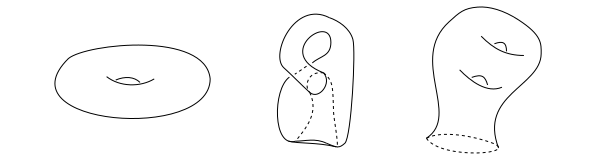
\includegraphics[width=1\textwidth]{reu_figures/surfaces.png}
    \label{fig:surfaces}
    \caption{Some popular examples of 2-dimensional manifolds: a torus, a Klein bottle and a punctured genus $2$ surface. Note that the torus is hollow.}
\end{figure}
For the remainder of this subsection, let $X$ be a Hausdorff, second countable topological space. These are technical hypotheses that we will not explore in depth. We will now define manifolds with boundary.

\begin{notation} (Upper Half-Space) For the remainder of these notes, we adopt the following notation and conventions.

The upper-half space $\R^{n-1} \times \R^+$ will be denoted by $\R^n_+$. The topological boundary of $\R^n_+$ as a subset of $\R^n$ will be denoted by $\partial \R^n_+$. The topological interior of $\R^n_+$ will be denoted as the compliment $\R^n_+\setminus \partial \R^n_+$.

A smooth function $f:U \to \R^k$ from an open subset $U \subset \R^n_+$ will, in these notes, mean a function of the form $f = g|_U$ where $V \subset \R^n$ is an open subset with $U = V \cap \R^n_+$ and $g:V \to \R^k$ is a smooth function in the usual sense. \end{notation}

\begin{definition} \label{def:charts_atlases} (Charts \& Atlases) An {\bf chart} $(U,\varphi)$ on the space $X$ is a pair of an open subset $U \subseteq X$ and a homeomorphism $\varphi:U \simeq V \subset \R^n_+$ from $U$ to an open subset $\varphi(U)$ of the upper half-space $\R^n_+$.

An {\bf atlas} $\mathcal{A}$ on $X$ is a set of charts $(U,\varphi)$ on $X$  satisfying these properties.
\begin{itemize} 
	\item[(a)] (Covering) The set of open sets occuring in charts of $\mathcal{A}$ is a cover of $X$.
	\item[(b)] (Chart Compatibility) If $(U,\varphi),(V,\psi) \in \mathcal{A}$ are two charts, then the {\bf transition function} defined as:
	\[\psi \circ \varphi^{-1}:\varphi(U \cap V) \simeq \psi(U \cap V)\]
	is smooth as a map between open subsets of $\R^n_+$.
\end{itemize}
An atlas $\mathcal{A}$ is {\bf maximal} if it is not a proper subset of another atlas. A maximal atlas on $X$ will also be referred to as a {\bf smooth structure} on $X$.
\end{definition}

\begin{definition} (Manifolds) \label{def:manifold} A {\bf smooth manifold with boundary} or is a Hausdorff, second countable topological space $X$ and a smooth structure $\mathcal{A}$ on $X$. 

A {\bf smooth manifold without boundary}, or simply {\bf manifold}, is a manifold with boundary such that every chart $(U,\varphi)$ in the atlas $\mathcal{A}$ is disjoint from the boundary $\partial \R^n_+$ of $\R^n_+$, in the sense that $\varphi(U) \cap \partial \R^n_+$ is empty. 
\end{definition}



\begin{definition} \label{def:maps_of_manifolds} (Maps Of Manifolds I) Let $M$ and $N$ be manifolds with boundary. 

\begin{itemize}
	\item[(a)] A {\bf (smooth) map} $f:X \to Y$ is a function such that the map of charts:
	\[\varphi \circ f \circ \psi^{-1}:\psi(U) \to \varphi(V)\]
	is a smooth map between the open subsets $\psi(U) \subset \R^m$ and $\varphi(V) \subset \R^n$, for any chart $(U,\psi)$ on $X$ and chart $(V,\varphi)$ on $Y$. 
	\item[(b)] An {\bf isomorphism} (or {\bf diffeomorphism}) $f:X \to Y$ is a bijective smooth map such that the inverse map $f^{-1}:Y \to X$ is also a smooth map.
\end{itemize}
\end{definition}

 \begin{remark}  \label{rmk:def:manifold} A few remarks are in order about Definition \ref{def:manifold}.
\begin{enumerate}
 \item[(a)] Usually we will just use $X$ to refer to the pair, omitting any notational reference to $\mathcal{A}$. When we refer to a chart $(U,\varphi)$ of $X$, we mean a chart in the corresponding atlas.
 \item[(b)] Any atlas $\mathcal{B}$ is contained in a unique maximal atlas $\mathcal{B}$ (a good {\bf Exercise}). Thus to specify a smooth structure, it suffices to specify a (not necessarily maximal) atlas on $X$ (although two atlases may specify the same smooth structure).
  \item[(c)] There is a notion of manifold that drops the hypothesis on the transition maps, so called topological manifolds. Most of the manifolds in these notes will be smooth, however, and we will note when this isn't the case.
   \item[(d)] A single topological space $X$ might carry \emph{multiple} smooth structures. This is not obvious! The first examples were constructed by Milnor \cite{milnor1956}, who found multiple smooth structures on the 7 dimensional sphere.
\end{enumerate}
 \end{remark}

 A manifold with boundary comes (unsurprisingly) with a subset called the boundary, which is itself a manifold \emph{without boundary}. 

 \begin{definition} (Boundary) Let $X$ be a manifold with boundary. The {\bf boundary} $\partial X$ of $X$ is the set of points $x \in X$ with the following property: there exists a chart $(U,\varphi)$ on $X$ such that $\varphi(x) \in \partial \R^n_+$. The {\bf interior} of $X$ is the complement $X \setminus \partial X$.
 \end{definition}

\begin{proposition} (Properties Of The Boundary) Let $X$ and $Y$ be a manifolds with boundary and $f:X \to Y$ be a smoooth map. 
\begin{itemize}
	\item[(a)] (Manifold Structure) $\partial X$ has a natural atlas induced by the atlas $\mathcal{A}$ of $X$. This atlas makes $\partial X$ into a manifold without boundary.
	\item[(b)] (Map Restriction) The map $f|_{\partial X}:\partial X \to Y$ is smooth. If $f(X) \subset \partial Y$ then, considered as a map to $\partial Y$, $f:X \to \partial Y$ is smooth.
	\item[(c)] (Tubular Neighborhood) There exists an open neighborhood $U \subset X$ of $
\partial X$ and a diffeomorphism $\varphi:\partial X \times [0,1) \simeq U$ such that $\varphi|_{X \times \{0\}}$ is the identity.
\end{itemize}
\end{proposition}

\begin{example} \label{ex:manifolds} Let us mention several examples of manifolds. For some of these spaces, we will not define the smooth structure now: rather, we will postpone the construction of the smooth structure to a section where we have more machinery.

\begin{enumerate}
	\item[(a)] (Euclidean Spaces) For any $n$, $\R^n$ has a natural smooth structure: an atlas is given by the single chart $(\R^n,\op{Id})$. 
	\item[(b)] (Spheres) For any $n$, the $n$-sphere $S^n$, defined as the set of points in $\R^{n+1}$ that are distance $1$ from the origin, has a natural smooth structure.
	\item[(c)] (Varieties) More generally, if $P(x)$ is a polynomial in $(n+1)$ variables $x_0,\dots,x_n$ and $\R$ coefficients, then $X := P^{-1}(0)$ is a manifold as long as $P$ satisfies:
	\[
	P(x) = 0 \implies \partial_i P(x) \neq 0 \text{ for some }
	\]
	\item[(d)] (Grassmanians) The space $\op{Gr}_\R(n,k)$ of all $k$-dimensional linear subspaces $P$ of $n$-space $\R^n$ can be given a natural manifold structure. These spaces are called \emph{Grassmanians}. One can also consider the \emph{complex Grassmanians} $\op{Gr}_\C(n,k)$ of all $k$-dimensional \emph{complex} linear subspaces $P$ of $\C^n$. Grassmanians are very elementary (but interesting) examples of so called {\bf moduli spaces}, i.e. spaces whose points are themselves spaces. 

	\item[(e)] (Projective Spaces) The spaces of lines $\op{Gr}_\R(n+1,1)$ and $\op{Gr}_\C(n+1,1)$ are called real and complex projective space, respectively, and denoted by $\R P^n$ and $\C P^n$.  

\end{enumerate} 
\end{example}

\begin{exercises} \label{exs:manifolds} Here are some basic exercises about manifolds.
\begin{enumerate}
	\item[(a)] Define an atlas on the sphere $S^n$ and verify the compatibility axiom.
	\item[(b)] Define atlases on the quotient group $\R/\Z$\footnote{By this we mean the space $\R$, quotiented by the equivalence relation that $x \sim y$ if and only if $x - y \in \Z$. The topology is defined as so: a set $U \subset \R/\Z$ is open if and only if the inverse image $\pi^{-1}(U)$ is open, where $\pi:\R \to \R/\Z$ is the map taking a point to its equivalence class.} and the projective space $\R P^1$ of lines in the real plane. Show that these spaces are diffeomorphic to $S^1$.
	\item[(c)] Suppose that $X$ is a connected topological space and has a manifold structure. The {\bf dimension} $\op{dim}(X)$ of $X$ is defined as so: let $(U,\varphi)$ be any chart, so that $\varphi(U) \subset \R^n$. Then $\op{dim}(X) = n$. Show that the dimension is well-defined. 

	(Hint: Reduce this to showing that you can't have a smooth map $\varphi:U \simeq V$ with smooth inverse $\varphi^{-1}:V \simeq U$ between open subsets $U \subset \R^m$ and $V \subset \R^n$ for $m \neq n$. To prove this reduction, consider the rank of the total derivative).
	\item[(d)] Brouwer proved the following result called \emph{Invariance of Domain}: Suppose that $U \subset \R^n$ is open and $f:U \to \R^n$ is an injective continuous map. Then $V = f(U)$ is open and $f$ is a homeomorphism between $U$ and $V$. 

	Use this result to prove that a continuous bijective map of manifolds (without boundary) has a continuous inverse. Thus we can define homeomorphisms of manifolds as continuous bijective maps.
\end{enumerate}
\end{exercises}

\subsection{Fiber And Vector Bundles} \label{subsec:fiber_bundles} Fiber bundles are spaces $E$ that are ``parameterized over a base'' $X$. Another way to think about them is that they are spaces that ``almost split'' into a product of two spaces, except there is a topological twist that gets in the way\footnote{I've heard (althogh I can't find a reference) that the historical Russian word for bundle translates literally as ``twisted product.''}. Vector bundles are special types of fiber bundles where the fibers are vector-spaces.
\vspace{5pt}
\begin{figure}[h]
    \centering
    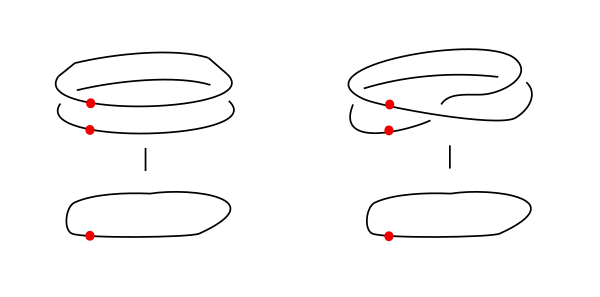
\includegraphics[width=.7\textwidth]{reu_figures/fiber_bundle.png}
    \label{fig:fiber_bundle}
    \caption{Two examples of fiber-bundles (with 2-point fiber) over the circle. A fiber and the accompanying base point are highlighted in red in both examples.}
\end{figure}

\begin{definition} \label{def:fiber_bundles} (Fiber Bundles) Let $X$ and $F$ be a smooth manifolds with boundary. A {\bf (smooth) fiber bundle} $E$ with {\bf base} $X$ and {\bf fiber} $F$ is a smooth manifold with boundary $E$ together with a projection map $\pi:E \to X$ such that:
\begin{itemize}
	\item[(a)] For every $x \in X$, there exists a neighborhood $U$ of $x$ and a diffeomorphism $\phi:E|_U \simeq U \times F$ such that $\pi|_U = \pi_1 \circ \phi$.
\end{itemize}
The inverse image $E_x := \pi^{-1}(x)$ for $x \in X$ is called the {\bf fiber at $x$}.
\end{definition}

\begin{definition} \label{def:vector_bundles} (Vector Bundles) Let $X$ be a smooth manifold with boundary and let $\mathbb{F}$ be either $\R$ or $\C$. A {\bf (smooth) vector bundle} $E$ with base space $X$ and fiber $\mathbb{F}^k$ is a fiber bundle such that:
\begin{itemize}
	\item[(a)] The fiber $E_x$ of a point $x \in X$ has a vector-space structure (i.e. addition and scalar multiplication) over $\mathbb{F}$.
	\item[(b)] For every $x \in X$, there exists a neighborhood $U$ of $x$ and a diffeomorphism $\phi:E|_U \simeq U \times \mathbb{F}^k$ such that $\pi|_U = \pi_1 \circ \phi$ and $\phi|_{E_x}:E_x \to \{x\} \times \mathbb{F}^k$ is linear.
\end{itemize}
The integer $k$ is called the {\bf rank} of $E$ and is denoted $\op{rank}(E)$.
\end{definition}

\begin{definition} \label{def:maps_of_fiber_bundles} (Maps Of Fiber Bundles) Let $\pi_A:A \to X$ and $\pi_B:B \to X$ be fiber bundles with fibers $F$ and $G$, respectively.
\begin{enumerate}
	\item[(a)] A {\bf bundle map} is a smooth map $f:A \to B$ and a smooth map $\underline{f}:X \to Y$ such that $\pi_B \circ f = \pi_A$. This means that $f$ preserves fibers, in the sense that the fiber $A_x$ of $x \in X$ is sent to the fiber $B_{x}$ by $f$. 
	\item[(b)] A {\bf bundle isomorphism} is a bundle map $f:A \to B$ that is a diffeomorphism.
	\item[(c)] A {\bf trivialization} of $A$ is a bundle isomorphism $f:A \simeq X \times F$. A bundle that admits a trivialization is called {\bf trivializable} or, colloquially, {\bf trivial}.
	\item[(c)] A {\bf section} $\sigma:X \to A$ of $A$ is a smooth map such that $\pi_A \circ \sigma = \op{Id}$. This means that it takes a point $x \in X$ to some point in the fiber $A_x$ of $x$. Note that every vector-bundle has a canonical section, the {\bf zero section}, given by $\sigma(p) = 0_p \in E_p$ where $0_p$ is the $0$ vector in $E_p$.

	The space of all smooth sections of a bundle $E$ is usually denoted by either $\Gamma(E), C^\infty(E)$, $\Gamma(X;E)$ or $C^\infty(X;E)$. If $E$ is a vector bundle then this space admits the structure of a topological vector-space.
\end{enumerate}
If $A$ and $B$ are vector bundles, we additionally stipulate that:
\begin{enumerate}
	\item[(a)] A bundle map must have fiber maps $f|_{A_x}:A_x \to B_{\underline{f}(x)}$ that are linear.
	\item[(b)] A bundle isomorphism must be linear bundle map in the above sense. 
\end{enumerate}
\end{definition} 

\begin{figure}[h!]
    \centering
    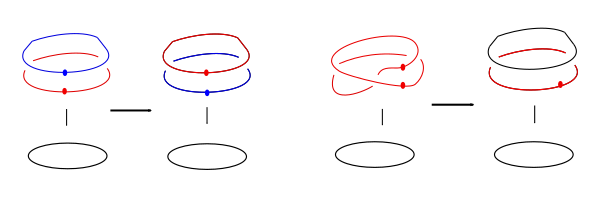
\includegraphics[width=1\textwidth]{reu_figures/maps_of_bundles_1.png}
    \label{fig:maps_of_bundles_1}
    \caption{This is a depiction of two bundle maps. In the leftward image, we have a bundle isomorphism from the trivial bundle with fiber $\{1,2\}$ to itself. The red and blue components on the far left are mapped right-wards to the component that is glowing the corresponding color. In particular, the two components are swapped. In the rightward image, we have a bundle map (which is \emph{not} an isomorphism) from the non-trivial $\{1,2\}$-bundle to the trivial $\{1,2\}$-bundle.}
\end{figure}

Given a smooth map $\varphi:X \to Y$, we can perform a sort of ``base change'' operation that takes bundles of $Y$ and turns them into bundles of $X$ by ``pulling back.'' We now describe this operation in detail.

\begin{definition} \label{def:pullback} (Pullback) Let $\varphi:X \to Y$ be a smooth map. 
\begin{itemize} 

	\item[(a)] (Pullback Bundle) The {\bf pullback bundle} $\varphi^*E$ associated to a bundle $E$ over $Y$ is the bundle with total space:
	\[
	\varphi^*E := \{(x,v) \in X \times E| v \in E_{\varphi(x)}\}
	\]
	The projection $\pi:\varphi^*B \to X$ given by the composition $\varphi^*B \subset X \times B \to X$ of inclusion and projection to the first factor.
	\item[(b)] (Pullback Bundle Map) The {\bf pullback bundle map} $\varphi^*f:\varphi^*D \to \varphi^*E$ associated to a bundle map $f:D \to E$ of bundles over $Y$ is defined as:
	\[
	\varphi^*f(x,v) = (x,f(v)) \in \varphi^*E \subset X \times E
	\]
	\item[(c)] (Pullback Section Map) The {\bf pullback section map} $\Gamma(\varphi):\Gamma(E) \to \Gamma(\varphi^*E)$ from sections of $E$ to sections of $\varphi^*E$ is defined so that the section $\sigma$ maps to the section of $\varphi^*E$ given by:
	\[
	\Gamma(\varphi)\sigma = (x,\sigma \circ \varphi(x)) \in \varphi^*E \subset X \times E
	\]
	By abuse of notation, we will generally denote this section by $\sigma \circ \varphi$. 
\end{itemize}
\end{definition}

\begin{proposition} \label{prop:pullback_properties} (Pullback Properties) The pullback operation $\varphi^*$ has the following properties.

\begin{enumerate}
	\item[(a)] (Composition) If $\varphi:X \to Y$ and $\psi:Y \to Z$ are smooth maps, $D$ and $E$ are vector-bundles on $Z$ and $f:D \to E$ is a bundle map, then:
	\[
	(\psi \circ \varphi)^*D = \varphi^*(\psi^*D) \qquad (\psi \circ \varphi)^*E = \varphi^*(\psi^*E)
	\]
	\[
	(\psi \circ \varphi)^*f = \varphi^*(\psi^*f)
	\]
	\item[(b)] (Trivial Pullbacks) The pullback $\varphi^*E$ of a trivial bundle $E$ is trivial.
\end{enumerate}
\end{proposition}

\begin{figure}[h]
    \centering
    \includegraphics[width=.5\textwidth]{reu_figures/maps_of_bundles_3.png}
    \label{fig:maps_of_bundles_3}
    \caption{Here we are depicting a bundle pullback. Note that this is only a completely accurate picture when the pullback map $\varphi$ is injective. On the right, we have a blue trivial bundle $B$ over a disk base $D$. On the bottom, there is a map of a red curve $C$ into the disk. The red region $R$ within the blue bundle is the pullback as it sits within $B$. The red region in the upper left is the total space of $f^*B$ itself.}
\end{figure}

\begin{example} \label{ex:bundles} Here are some examples of fiber bundles. Many more examples will be discussed in the next section.
\begin{enumerate}
	\item[(a)] (Trivial Example) If $X$ and $F$ are smooth manifolds, then $\pi_X:X \times F \to X$ is a fiber bundle with projection $\pi_X:X \times F \to X$ given by projection to the first factor.
	\item[(b)] (Non-Trivial Bundles On Circle) Let $X = S^1$ be the circle. By identifying $S^1$ with the unit complex numbers, we have for each $k \in \Z^+$ a ``$k$-fold covering map'':
	\[
	\pi_k:S^1 \to S^1 \quad e^{i\theta} \mapsto e^{ik\theta}
	\]
	Thus we can take $E_k = S^1$ to get a fiber bundle $\pi_k:E_k \to S^1$ for each $k$, with fiber isomorphic to the finite set $\{1,\dots,k\}$.
	\item[(c)] (Tautological Bundles On $\R P^n$) Consider projective space $\R P^n$, the space of lines $L$ in $\R^{n+1}$. We can define vector bundle $E \to \R P^n$ with fiber $\R$ as a subset of $\R P^n \times \R^{n+1}$ in the following way:
	\[
	E_n := \{(L,v) \in \R P^n \times \R^{n+1}| v \in L \subset \R^{n+1}\}
	\]
	Projection is defined by composing the inclusion $E \subset \R P^n \times \R^{n+1}$ with projection to the first factor. Similarly, we can define a bundle $U \to \R P^n$ with fiber $\{1,2\}$ of two points by setting:
	\[
	U_n := \{(L,v) \in \R P^n \times \R^{n+1}| v \in L \subset \R P^{n+1} \text{ and }|v| = 1\}
	\]
\end{enumerate}
\end{example}

\begin{exercises} \label{exs:bundles} Here are some exercises about bundles.
\begin{itemize}
	\item[(a)] Show that the bundles $\pi_k:E_k \to S^1$ in Examples \ref{ex:bundles}(b) are not trivial (i.e., not bundle isomorphic to the trivial bundle with the same fiber) when $k > 1$. (Hint: Consider the topological properties of the total space $E_k$).
	\item[(b)] In Exercise \ref{exs:manifolds}(b), the reader was asked to construct a diffeomorphism $\underline{\varphi}:\R P^1 \simeq S^1$. Show that the bundle $U_1 \to \R P^1$ given in Example \ref{ex:bundles}(c) is bundle isomorphic to the bundle $\pi_2:\underline{\varphi}^*E_2 \to \R P^1$ of $E_2 \to S^1$ as defined in Example \ref{ex:bundles}(b).
	\item[(c)] Show that the pullback of a trivial bundle is also trivial. 
	\item[(d)] Give an example of a non-trivial bundle $E \to Y$ and a map $f:X \to Y$ such that $f^*E$ is trivial.
	\item[(e)] Prove that the bundles $U_n \to \R P^n$ are non-trivial. Hint: Show that there is an inclusion $\iota:\R P^1 \to \R P^n$ and show that $\iota^*U_n$ is non-trivial using (a).
	\item[(f)] Explain why a rank $1$ vector bundle is trivial if and only if it has a non-vanishing section. Generalize this statement to bundles of higher rank and prove the generalized statement.
\end{itemize}
\end{exercises} 

\subsection{Review Of Linear Algebra} \label{subsec:review_of_linear_algebra} Given a vector bundle $E$, one can construct many new bundles naturally associated to $E$ by applying linear algebraic constructions (which make sense on plain vector-spaces) to vector bundles in a smooth and fiber-wise way. In this section, we will review the linear algebra prerequisites that we will need for this discussion. This material should be standard in an advanced linear algebra course.

The format of this section will be as so. We will review five constructions: direct sums, tensor products, (spaces of) linear maps, dual spaces and exterior algebras. For each concept, we will first review the definition and the key properties. We will then provide some intuition about the construction and a picture.

Through out this section, let $\mathbb{F}$ be either $\R$ or $\C$ (although much of this material will work for any ring $R$, where we replace vector-spaces with modules). Let $U,V$ and $U',V'$ be $\mathbb{F}$ vector-spaces and let $\varphi:U \to U'$ and $\psi:V \to V'$ be a linear maps. 

\begin{review} \label{rev:direct_sum_and_tensor_product} (Direct Sum \& Tensor Product) The {\bf direct sum} $U \oplus V$ is the vector-space of pairs $u \oplus v$ equipped with term-wise addition and scalar multiplication:
\[u \oplus v + t \oplus w = (u + t) \oplus (v + w)\]
\[c(u \oplus v) = (cu) \oplus (cv)\]
The maps $\varphi$ and $\psi$ induce a map $\varphi \oplus \psi:U \oplus V \to U' \oplus V'$ given by:
\[
u \oplus v \mapsto \varphi u \oplus \psi v
\]
The {\bf tensor product} $U \otimes V$ is defined as the vector-space generated by pairs $u \otimes v$ subject to the relations:
	\[(u + t) \otimes v = u \otimes v + t \otimes v \text{ for all $t,u \in U$ and $v \in V$}\]
	\[u\otimes (v + w) = u \otimes v + u \otimes w \text{ for all $u \in U$ and $v,w \in V$}\]
	\[ c(u \otimes v) = (cu) \otimes v = u \otimes (cv) \quad \text{ for }c \in \mathbb{F}\]
A vector $x$ in a tensor product is often called {\bf tensor}. An tensor of the form $x = u \otimes v$ for $u \in U$ and $v \in V$ is called a {\bf pure tensor}.  The maps $\varphi$ and $\psi$ induce a map $\varphi \otimes \psi:U \otimes V \to U' \otimes V'$ defined on pure tensors as:
\[u \otimes v \mapsto \varphi u \otimes \psi v\]
The direct sum $\oplus$ and tensor product $\otimes$ have the following properties.
\begin{itemize}
	\item[(a)] (Tensor Universal Property) Let $\op{Bil}(U,V;W)$ denote the space of maps $f:U \times V \to W$ that are bilinear, i.e. linear in each variable. Then $\op{Hom}(U \otimes V,W) \simeq \op{Bil}(U,V;W)$ via the canonical map:
	\[
	\varphi \in \op{Hom}(U \otimes V,W) \mapsto ((u,v) \mapsto \varphi(u \otimes v)) \in \op{Bil}(U,V;W)
	\]
	In particular, to specify a map $U \otimes V \to W$, it suffices to specify a map on pure tensors $u \otimes v \mapsto B(u,v)$ where $B:U \times V \to W$ is bilinear. For (a)-(g), we specify all maps from tensor products in terms of pure tensors in this way.

	\item[(b)] (Associativity) $U \oplus (V \oplus W) \simeq (U \oplus V) \oplus W$ and $U \otimes (V \otimes W) \simeq (U \otimes V) \otimes W$ via the canonical isomorphisms:
	\[u \oplus (v \oplus w) \mapsto (u \oplus v) \oplus w \qquad u \otimes (v \otimes w) \mapsto (u \otimes v) \otimes w\]
	\item[(c)] (Commutativity) $U \oplus V \simeq V \oplus U$ and $U \otimes V \simeq V \otimes U$ via the canonical isomorphisms:
	\[ u \oplus v \mapsto v \oplus u \qquad u \otimes v \mapsto v \otimes u\]
	\item[(d)] (Distributivity) $U \otimes (V \oplus W) \simeq (U \otimes V) \oplus (U \otimes W)$ via the canonical isomorphism:
	\[u \otimes (v \oplus w) \mapsto (u \otimes v) \oplus (u \otimes w)
	\]
	\item[(e)] (Unit) Let $Z = \{0\}$ be the zero vector space and $\mathbb{F}$ be the base field as a vector space. Then $Z \oplus U \simeq U$ and $\mathbb{F} \otimes U \simeq U$ via the canonical isomorphisms:
	\[
	0 \oplus u \mapsto u \qquad c \otimes u \mapsto cu
	\]
	\item[(f)] (Hom Additivity) $\op{Hom}(U,W) \oplus \op{Hom}(V,W) \simeq \op{Hom}(U \oplus V,W)$ (and similarly for the second entry) via the canonical isomorphism:
	\[
	A \oplus B \mapsto (u \oplus v \mapsto Au + Bv)
	\]
	\item[(g)] (Tensor-Hom Adjunction) $V \otimes U^* \simeq \op{Hom}(U,V)$ via the canonical isomorphism:
	\[
	v \otimes \alpha \mapsto (u \mapsto \alpha(u) v)
	\]
\end{itemize}
\end{review}

\begin{motivation} Direct sums are fairly simple to understand, but tensor products are (at first glance) rather opaque. What is a tensor product supposed to be? One of our favorite ways to think about tensor products is as so:
\begin{center}
\emph{a tensor is like a matrix, but shaped like a cube (or hyper-cube) instead of a square}
\end{center}
What do we mean by this? Well, suppose that $\{e_i\}_{i=1}^n$ is a basis of a vector space $V$. One can show then that the pure tensors $e_i \otimes e_j$ form a basis for $V \otimes V$. Then every tensor $x$ can be written uniquely as:
\[
x = \sum_{i,j} a_{ij} e_i \otimes e_j
\]
Here $a_{ij}$ are coefficients in $\mathbb{F}$. We then can interpret the numbers $a_{ij}$ as entries of a matrix $A = [a_{ij}]$. Similarly, if we tensor together 3 different vector-spaces $U \otimes V \otimes W$ with bases $\{e_i\}, \{f_j\}$ and $\{g_k\}$, then $\{e_i \otimes f_j \otimes g_k\}$ is a basis of the tensor product and any tensor $x \in U \otimes V \otimes W$ can be written as:
\[
x = \sum_{i,j,k} a_{ijk} e_i \otimes f_j \otimes g_k
\]
Thus we can interpret $x$ in these bases as a cube-shaped array of numbers. 

The point here is that $U \otimes V \otimes W$ is like a space of cube shaped matrices with three ``directions''; the $U$ direction, the $V$ direction and the $W$ direction.
\end{motivation} 

\begin{review} \label{rev:morphism_spaces} (Morphism Spaces) The {\bf morphism space} $\op{Hom}(U,V)$ between $U$ and $V$ is the vector-space of linear maps from $U$ to $V$. The {\bf isomorphism space} $\op{Iso}(U,V) \subset \op{Hom}(U,V)$ is the open subset of invertible linear maps. The maps $\varphi$ and $\psi$ induce an map $\op{Hom}(\psi,\varphi):\op{Hom}(U',V) \simeq \op{Hom}(U,V')$ defined as:
\[
f \mapsto \psi \circ f \circ \varphi
\] 
The morphism spaces come with the following additional structure.

\begin{enumerate} 
	\item[(a)] (Application) A linear map $\op{Hom}(U,V) \otimes U \to V$ given by $f \otimes u \mapsto f(u)$.
	\item[(b)] (Composition) A linear map $\op{Hom}(U,V) \otimes \op{Hom}(V,W) \to \op{Hom}(U,W)$ given by $f \otimes g \mapsto g \circ f$.
\end{enumerate} 
\end{review}

\begin{review} \label{rev:dual_spaces} (Dual Space) The {\bf dual space} $U^*$ of $U$ is the vector-space $\op{Hom}(U,\mathbb{F})$ of linear maps from $U$ to $\mathbb{F}$. $\varphi$ induces a map $\varphi^*:(U')^* \to U^*$ defined by the pullback formula (b) below. The dual space comes equipped with the following additional structure and properties.
\begin{enumerate} 
	\item[(a)] (Dual Pairing) A linear map $U^* \otimes U \to \mathbb{F}$ given by $(\alpha,u) \mapsto \alpha(u)$.
	\item[(b)] (Pullback) A linear map $\op{Hom}(U,V) \otimes V^* \to U^*$ given by $(f,\alpha) \mapsto \alpha \circ f$. $\alpha \circ f$ is also denoted by $f^*\alpha$.
	\item[(c)] (Double Dual) The double dual $(U^*)^*$ has a canonical isomorphism $U \simeq (U^*)^*$ given by:
	\[u \mapsto (\alpha \mapsto \alpha(u))\]
\end{enumerate}
\end{review}

\begin{review} \label{rev:exterior_algebra}(Exterior Algebra) The {\bf exterior algebra} $\Lambda U$ is the algebra with product $\wedge$ generated as an algebra by the scalars $c \in \mathbb{F}$ and vectors $u \in U$, which are subject to the relations:
	\[
	u \wedge v = - v \wedge u \text{ for any }u,v \in U \qquad c \wedge u = cu \text{ for any }c \in \mathbb{F} \text{ and }u \in U
	\]
	Note that the products of algebras are associative and bilinear. The latter means we have the identity:
	\[
	(u + v) \wedge w = u \wedge w + v \wedge w \quad\text{and}\quad u \wedge (v + w) = u \wedge v + u \wedge w \text{ for any }u,v,w \in \Lambda U
	\]
The map $\varphi$ induces an map $\Lambda \varphi:\Lambda U \to \Lambda U'$ given by:
\[
u_1 \wedge \dots \wedge u_k \mapsto (\varphi u_1) \wedge \dots \wedge (\varphi u_k)
\]
The exterior algebra comes equipped with the following structure.

\begin{itemize}
	\item[(a)] (Grading) A decomposition $\Lambda U = \bigoplus_{k=0}^{\op{dim}(U)} \Lambda^kU$. Here $\Lambda^0 U = \mathbb{F} \subset \Lambda U$ and $\Lambda^k U$ is (for $k > 0$) the span of the elements $\alpha \in \Lambda U$ of the form $\alpha = u_1 \wedge \dots \wedge u_k$. Note, in particular, that $\Lambda^1 U \simeq U$ canonically.

	An $x \in \Lambda^k V$ is said to have {\bf degree} $k$. The degree of $x$ is denoted $\op{deg}(v)$.
 	\item[(b)] (Exterior Product) A product map $\Lambda U \otimes \Lambda U \to \Lambda U$ given by $u \otimes v \mapsto u \wedge v$ that is compatible with the decomposition from (a) in the sense that if $\alpha \in \Lambda^j U$ and $\beta \in \Lambda^k U$ then:
	\[
	\alpha \wedge \beta = (-1)^{ij} \beta \wedge \alpha
	\]
	Note that $c \wedge \alpha = c\alpha$ for $c \in \Lambda^0 U = \mathbb{F}$.
	\item[(c)] (Interior Product) A linear map $U^* \otimes \Lambda  U \to \Lambda U$, denoted by $u \otimes \alpha \mapsto \iota(u) \alpha$ or by $(u,\alpha) \mapsto i_u \alpha$, and defined uniquely by the following properties.
	\begin{itemize}
		\item[-] (Degree 0 \& 1) For $c \in \Lambda^0 U, \alpha \in \Lambda^1 U$ and $u \in U^*$, we have:
		\[\iota_u c = 0 \qquad \iota_u \alpha = u(\alpha)\]
		\item[-] (Leibniz Rule) For $\alpha \in \Lambda^j U, \beta \in \Lambda^k U$ and $u \in U^*$, we have:
		\[\iota_u(\alpha \wedge \beta) = (\iota_u \alpha) \wedge \beta + (-1)^j \alpha \wedge (\iota_u \beta)\]
	\end{itemize} 
	Note that of we let $U = V^*$, so that $U^* = (V^*)^* \simeq V$, the interior product is instead a map $\iota:V \otimes \Lambda V^* \to V$. 
	\item[(d)] (Anti-Symmetric Multi-Linear Forms) Let $\op{Asym}_k(V)$ denote the vector-space of anti-symmetric $k$-linear forms on $V$. That is, an element $A \in \op{Asym}_k(V)$ is a map $A:\times_1^k V \to \mathbb{F}$ such that for any permutation $\sigma:\{1,\dots,k\} \to \{1,\dots,k\}$:
	\[
	A(v_{\sigma(1)},\dots,v_{\sigma(k)}) = (-1)^{\op{sign}(\sigma)} \cdot A(v_1,\dots,v_k)
	\]
	Where $\op{sign}:\Sigma_k \to \{\pm 1\}$ is the usual sign of a permutation $\sigma \in \Sigma_k$. Then $\Lambda^k V^* \simeq \op{Asym}_k(V)$ via the natural isomorphism:
	\[
	\omega \mapsto A \qquad A(v_1,\dots,v_k) := \iota(v_k)\iota(v_{k-1})\dots \iota(v_1)\omega \in \Lambda^0V^* \simeq \mathbb{F}
	\]
	Given a map $f:U \to V$, we get a map $f^*:V^* \to U^*$ and thus a map $\Lambda(f^*):\Lambda V^* \to \Lambda U^*$ sending $\Lambda^kV^*$ to $\Lambda^k U^*$. Under the identifications $\Lambda^k U^* \simeq \op{Asym}_k(U)$ and $\Lambda_k V^* \simeq \op{Asym}(V)$, this map corresponds to the map:
	\[
	f^*:\op{Asym}_k(V) \to \op{Asym}_k(U) \qquad [f^*A](v_1,\dots,v_k) = A(f(v_1),\dots,f(v_k))
	\]
\end{itemize}

\begin{remark} \label{rmk:dual_exterior_algebra} For our purposes, the exterior algebra $\Lambda^k V^*$ of the dual $V^*$ will be much more important that the exterior algebra of $V$ itself. In particular, the interpretation of elements $\omega \in \Lambda^k V^*$ as anti-symmetric multi-linear forms, as allowed by Review \ref{rev:exterior_algebra}(d) above, will be used constantly. 
\end{remark}

\begin{motivation} \label{mot:exterior_algebra} The exterior algebra is another construction that, like the tensor product, can be very difficult to understand when first encountered. We will now provide some intuition for this. It is easiest to understand things using the exterior algebra of the dual $\Lambda^k V^*$, and per Remark \ref{rmk:dual_exterior_algebra} this is really better for us anyway.

First, consider an element $\nu \in \Lambda^n (\R^n)^*$. By Review \ref{rev:exterior_algebra}(d), $\nu$ corresonds to an $n$-linear, anti-symmetric form $A_\nu \in \op{Asym}_n(\R^n)$. What is an example of such a form? One example is:
\[
A_1(v_1,\dots,v_n) = \op{det}([v_1|v_2|\dots|v_n])
\]
Here $M(v) := [v_1|v_2|\dots|v_n]$ is the matrix whose columns are the vectors $v_i$. The geometric interpretation of this form is clear: if $Q$ represents the cube with unit length edges and $P(v) = M(v)Q$ represents the (higher dimensional) parallelepiped made by applying $M(v)$ to $Q$, then:
\[
A_1(v_1,\dots,v_n) = \pm \op{volume}(P(v))
\]

We should interpret $A_\nu$ similarly: $A_\nu$ is a like a ``volume measuring stick'' or a ``choice of volume scale.'' If you provide $A_\nu$ with a parallelepiped $P(v)$, $A_\nu$ spits out a number $A_\nu(v_1,\dots,v_n)$ that measures the ``signed size'' of $P(v)$ in the units of $A_\nu$. This ``signed size'' has many of the same formal properties as the usual determinant: for instance, if you switch around the order of the vectors $(v_1,\dots,v_n)$, the determinat $\op{det}([v_i])$ changes by a sign (because the volume of the parallelepiped $P(v)$ stays the same). The quantity $A_\nu$ behaves similarly.

Now let's consider a general $\nu \in \Lambda^k V^*$. Again, if $k = \op{dim}(V)$, we interpret $\nu$ as specifying a sort of signed volume scale on $V$ via the $k$-linear form $A_\nu$. If $k < n$, then we can consider any dimension $k$-subspace. Then by Review \ref{rev:exterior_algebra}(4), we have a map $\iota^*:\Lambda^k(V^*) \to \Lambda^k(P^*)$ given by the inclusion $\iota:P \hookrightarrow V$. Then since $\iota^*\nu$ is on $P$ and $P$ is $k$-dimensional, $\iota^*\nu$ can be interpreted as a way of measuring volume on $P$. Thus we have the following intuition:
\begin{center}
\emph{An element $\nu \in \Lambda^k(V^*)$ is, intuitively, an assignment of an (signed) area scale to each $k$-dimensional subspace $P \subset V$.} 
\end{center}
\end{motivation}

\begin{figure}[h]
    \centering
    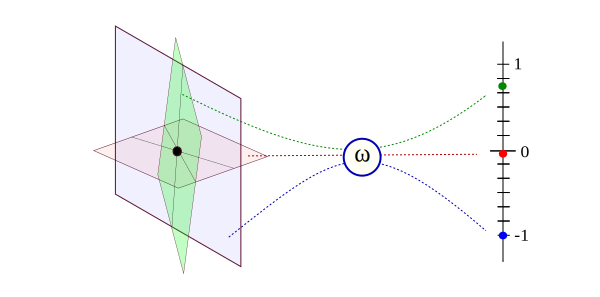
\includegraphics[width=\textwidth]{reu_figures/exterior_algebra.png}
    \label{fig:exterior_algebra}
    \caption{A picture of what a $k$-form (in this case, a $2$-form $\omega$) does. In this picture, we have 3 $2$-dimensional rectanges (red, green and blue) in a $3$-dimensional space $V$. $\omega$ takes those rectangles (with a big of extra information) and assigns them a signed area, given on the right by the dot of the corresponding color.}
\end{figure}

The final topic of discussion for this sub-section is that of orientations. This is a somewhat non-standard topic in linear algebra courses, even the theoretically oriented ones, so the reader may be seeing this construction for the first time.

\begin{definition} \label{def:orientation_space} The {\bf orientation space} $\mathfrak{o}U$ of a vector-space is the set:
\[
\mathfrak{o}U := (\Lambda^n U - 0)/\R^+
\]
That is, an element $[\mu] \in \mathfrak{o}U$ is an equivalence class of vector $\mu \in \Lambda^n U$ modulo scaling by a non-negative constant $\lambda \in \R^+$. An element $o \in \mathfrak{o}U$ is called an {\bf orientation} of $U$. The orientation space has the following properties:
\begin{enumerate}
	\item[(a)] ($\Z/2\Z$-action) $\mathfrak{o}U$ has a $\mathbb{Z}/2\Z$ action given by $k \cdot [\mu] = [(-1)^k\mu]$ for $k \in \Z/2\Z$. Furthermore, this action is free and transitive.
	\item[(b)] (Isomorphisms) An \emph{isomorphism} $\varphi:U \simeq U'$ induces an \emph{isomorphism} $\mathfrak{o}\varphi:\mathfrak{o}U \simeq \mathfrak{o}U'$ given by $[u] \mapsto [\Lambda\varphi(u)]$ that commutes with the $\Z/2\Z$ action. Note that an arbitrary map $\varphi$ does not induce a map $\mathfrak{o}\varphi$ of any sort.
\end{enumerate}
\end{definition}

\begin{motivation} 
\end{motivation} 

\begin{exercise} \label{ex:linear_algebra} Here are some linear algebra exercises dealing with the constructions that were reviewed in this chapter. Let $U,V$ and $W$ be vector-spaces throughout. Also assume that $V$ is dimension $n$.

\begin{itemize}
	\item[(a)] $\op{Sym}_k(V)$ is the vector-space of $k$-linear maps to $\mathbb{F}$ from $V$ that are symmetric in each entry. Compute the dimension of $\Lambda^k V$ and $\op{Sym}_k(V)$ for each $k$. 
	\item[(b)] Show, by applying (a), that the determinant map:
	\[(v_1,\dots,v_n) \mapsto \op{det}([v_1|\dots|v_n])\]
	is the unique anti-symmetric, $n$-linear map $\times_1^n \R^n \to \R$ whose value is $1$ on $(e_1,\dots,e_n)$ (where $\{e_i\}$ is the standard basis).
	\item[(c)] Show, by applying (b), that the map $\Lambda \varphi:\Lambda^n V \to \Lambda^n V$ induced by a linear map $\varphi:V \to V$ is just the map $\mu \mapsto \op{det}(\varphi) \cdot \mu$. Deduce that the map $\mathfrak{o}\varphi:\mathfrak{o}V \to \mathfrak{o}V$ is given by $[\mu] \mapsto \op{sign}(\op{det}(\varphi)) \cdot [\mu]$.
	\item[(d)] Show that the wedge product $\wedge$ on $\Lambda V$ is graded commutative: that is, show that if $\alpha \in \Lambda^j V$ and $\beta \in \Lambda^k V$, then $\alpha \wedge \beta = (-1)^{jk} \beta \wedge \alpha$.
	\item[(e)] Prove the following stronger version of the tensor-hom adjunction property in Review \ref{rev:direct_sum_and_tensor_product}:
	\[
	\op{Hom}(U, V \otimes W) \simeq \op{Hom}(\op{Hom}(V,U),W)
	\]
	\item[(f)] Show that $\iota_v \iota_w \alpha + \iota_w \iota_v \alpha = 0$. In particular, $\iota_w^2\alpha = 0$.
\end{itemize}
\end{exercise}

\end{review}
\subsection{Constructions Of Bundles} \label{subsec:natural_constructions_of_bundles} As we stated at the begining of \S \ref{subsec:review_of_linear_algebra}, the constructions discussed in that section can be extended to operations on vector bundles. Here is an informal statement of how this works.

\begin{theorem} \label{thm:informal_bundles} (Informal Vector Spaces $\implies$ Bundles) Every operation for vector spaces in \S \ref{subsec:review_of_linear_algebra} can be converted into an analogous operation on vector bundles over a fixed base $X$. The following table provides a dictionary for term-to-term translation of the properties of a vector-space operation into properties of the correspondign bundle operation.
\end{theorem} 

\begin{center}
\begin{tabular}{c|c}
vector spaces & vector bundles over $X$\\
\hline 
canonical linear maps & canonical bundle maps\\
\hline
canonical isomorphisms & canonical bundle isomorphisms\\
\hline
base field $\mathbb{F}$ & trivial bundle $X \times \mathbb{F}$\\
\end{tabular}
\end{center}

It may be helpful for the reader to see an example of this principal. Let us therefore state a version of Review \ref{rev:dual_spaces} for bundles. 

\begin{example} \label{ex:bundle_dual} (Bundle Dual) Let $E$ and $F$ be a bundles over a manifold $X$, and let $\varphi:E \to E'$ be a bundle isomorphism.

The {\bf dual bundle} $E^*$ of $E$ is the vector bundle $\op{Hom}(E,X \times \mathbb{F})$ of (fiberwise) linear maps from $E$ to $\mathbb{F}$. The bundle isomorphism $\varphi$ induces a bundle isomorphism $\varphi^*:(U')^* \to U^*$. The dual bundle comes equipped with the following additional structure and properties.
\begin{enumerate} 
	\item[(a)] (Dual Pairing) A linear bundle map $U^* \otimes U \to X \times \mathbb{F}$ given by $\alpha \otimes u \mapsto \alpha(u)$ fiberwise.
	\item[(b)] (Pullback) A linear bundle map $\op{Hom}(U,V) \otimes V^* \to U^*$ given by $f \otimes \alpha \mapsto \alpha \circ f$ fiberwise. $\alpha \circ f$ is also denoted by $f^*\alpha$.
	\item[(c)] (Double Dual) The double dual $(E^*)^*$ has a canonical bundle isomorphism $E \simeq (E^*)^*$ given fiberwise by:
	\[u \mapsto (\alpha \mapsto \alpha(u))\]
\end{enumerate}
\end{example}

The informal statement of Theorem \ref{thm:informal_bundles} discussed above is often sufficient for the working mathematician. However, we now state a careful Proposition explaining how this conversion actually works. The proof of this statement is long, so we defer it to Appendix \ref{appendix:proofs_for_manifold_basics}.

\begin{remark} Note that there is a version of the following statement for tuples of vector bundles that could probably incorporate every case that we are interested in, but to reduce the complexity of notation and everything, we have avoided this generalization. It is very similar to the version that we are about to describe.
\end{remark}

\begin{proposition} \label{prop:general_bundle_operations} Let $F$ be an operation on vector spaces with these properties.
\begin{itemize}
\item[(a1)] (Object Map) $F$ associates a new vector-space $F(V)$ to any vector-space $V$. 
\item[(a2)] (Morphism Map) $F$ associates a linear map $F(f):F(U) \to F(V)$ to any linear map $f:U \to V$. 
\item[(a3)] (Composition) $F(f \circ g) = F(f) \circ F(g)$ for linear maps $f$ and $g$.
\item[(a4)] (Smoothness) The map $\op{Hom}(U,V) \to \op{Hom}(F(U),F(V))$ given by $\varphi \mapsto F(\varphi)$ is smooth as a map between vector-spaces. 
\end{itemize}
Then there is unique\footnote{In the sense of Exercise \ref{ex:bundle_constructions}(c)} operation $F$ on vector bundles with the following properties.
\begin{itemize}
\item[(b1)] (Object Map) $F$ associates a vector bundle $F(E)$ to any vector bundle $E$. 
\item[(b2)] (Morphism Map) $F$ associates a bundle map $F(f):F(D) \to F(E)$ to any bundle map $f:D \to E$. 
\item[(b3)] (Composition) $F(f \circ g) = F(f) \circ F(g)$ for bundle maps $f$ and $g$. 
\item[(b4)] ($F(E)$ Trivial On Trivial Bundles) For a trivial vector bundle $X \times V$, there is a natural isomorphism $F(X \times V) \simeq X \times F(V)$.
\item[(b5)] ($F(f)$ Standard On Trivial Bundles) If $f:X \times U \to X \times V$ is a bundle map of trivial bundles, then we can write $f$ as:
\[
f(x,v) = (x,f_x(v))
\]
Here $x \mapsto f_x$ is a smooth map $X \to \op{Hom}(U,V)$ from $X$ to the space of linear maps from $U$ to $V$. Then under the identifications of $F(X \times U) \simeq fX \times F(U)$ and $F(X \times V) \simeq X \times F(V)$, we have:
\[
f(x,u) = (x,F(f_x)u) \in Y \times F(V) \simeq F(Y \times V)
\]
\end{itemize}
\end{proposition}

 Here is the idea behind the proof: we construct $F(E)$ as a certain type of quotient space, by taking \emph{all} of the local trivializations provided by the vector-bundle axiom, applying the construction of $F$ to each trivialization, and then gluing it all together. 

\begin{exercise} \label{ex:bundle_constructions} Here are some exercises for the reader dealing with all of the bundle nonsense discussed in this section. 

\begin{enumerate}
	\item[(a)] Let $\pi:L \to X$ be a vector bundle of rank $1$ over $X$. Show that the bundle $\op{End}(L)$ of maps from $L$ to itself is trivializable. (Hint: Find a section then use Exercise \ref{exs:bundles}(f)).
	\item[(b)] Let $D$ and $E$ be two vector bundles with base $X$. Given a section $A:X \to \op{Hom}(D,E)$ of the morphism bundle $\op{Hom}(D,E)$, we can produce a bundle map $f_A:D \to E$ by applying $A$ to $D$ fiberwise. That is:
	\[f_A(x,v) = (x,A_xv)\]
	Show that, conversely, every bundle map $f:D \to E$ can be associated to a unique section $A$ of $\op{Hom}(D,E)$.
	\item[(c)] Show that the extension of an operation $F$ from vector-spaces to vector-bundles (as described in Proposition \ref{prop:general_bundle_operations}) is unique in the following sense, using only Properties \ref{prop:general_bundle_operations}(b1)-(b5).

	If $F$ and $F'$ are two operations on vector bundles satisfying Properties \ref{prop:general_bundle_operations}(b1)-(b5), then there is a canonical isomorphism $\tau_E:F(E) \simeq F'(E)$ with the following property: for any bundle map $f:D \to E$, $F(f)$ and $F'(f)$ are related by $F(f) \circ \tau_D = \tau_E \circ F'(f)$.

	Note that you \emph{do not} need to know the proof of Proposition \ref{prop:general_bundle_operations}.



\end{enumerate}
\end{exercise}

\subsection{Natural Bundles On Smooth Manifolds} \label{subsec:natural_bundles_on_manifolds} Smooth manifolds have many natural vector bundles and fiber bundles associated to them. Indeed, this is one the main ways that bundles arise in mathematical nature. These bundles are usually made by applying some of the natural operations discussed in \S \ref{subsec:natural_constructions_of_bundles} to the tangent bundle.

\begin{motivation} What is that tangent bundle intuitively? Near a point $x$, $X$ looks locally like a flat space, i.e $\R^n$ for some $n$. There is a space of ``infinitesimal directions'' that one can travel out from $x$: these are the vectors that are ``tangent the the manifold at $x$'', and the vector-space populated by these vectors is the tangent space $TX_x$, the fiber of the tangent bundle at $x$. The tangent bundle arises when one joins all of these tangent spaces together into a single space.

We will see later that, when the manifold $X$ sits inside of another manifold (say, some Euclidean space $\R^m$) in a sufficiently nice way, then the tangent space $TX_x$ at a point is literally the space of vectors in $\R^m$ that are tangent to $X$ in $\R^m$. \end{motivation}

\begin{figure}[h]
    \centering
    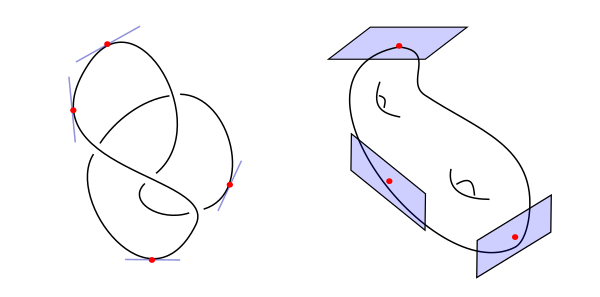
\includegraphics[width=.9\textwidth]{reu_figures/tangent_bundles.png}
    \label{fig:tangent_bundle}
    \caption{A pair of manifolds sitting in $\R^3$, a curve (left) and a surface (right). The red dots are points on the manifolds and the blue lines/planes are the tangent spaces at those points. The tangent bundle is made by putting all of these blue tangent spaces together into a single bundle.}
\end{figure}

\begin{proposition} \label{def:bundles_on_smooth_manifolds} (Bundles On Smooth Manifolds) Let $X$ be a smooth manifold. Then we can associate the following bundles to $X$.
\begin{enumerate}
	\item[(1)] (Tangent Bundle) The tangent bundle can be defined in terms of an operation $T$ associating a bundle $TX$ to any manifold $X$. This operation exists and satisfies the following axioms.
	\begin{itemize}
	\item[(a)] (Object Map) $T$ associates a smooth vector bundle $TX$ to any smooth manifold $X$. $TX$ is called the {\bf tangent bundle} of $X$.
	\item[(b)] (Morphism Map) $T$ associates a bundle map $Tf:TX \to f^*TY$ between $TX$ and the pullback of $TY$ by $f$ to any any smooth $f:X \to Y$.
	\item[(c)] (Composition) $T$ respects composition: $T(g \circ f) = f^*(Tg) \circ Tf$.
	\item[(d)] ($TV$ Is $V \times V$ On Vector-Spaces) $TV \simeq V \times V$ canonically for any vector space $V$. Here $V \times V$ is of course the trivial bundle with fiber $V$. 
	\item[(e)] ($Tf$ Is Jacobian On Vector-Spaces) If $f:U \to V$ is a smooth map between vector-spaces, then via the identification in (c), we have $f^*TV \simeq U \times V$ and:
	\[
	Tf(x,v) = (x,df_x(v)) \in U \times V \simeq f^*TV
	\]
	Here $df_x$ is the Jacobian of $f$ at $x$.
	\end{itemize}
	A section $Z$ of the tangent bundle is called a {\bf vector-field}.

	\item[(2)] (Cotangent Bundle) The cotangent bundle $T^*X$, defined to be the dual bundle to $TX$. Like $TX$, $T^*X$ can be defined in terms of an operation $T^*$ associating a bundle $T^*X$ to any manifold $X$ that satisfies analogous axioms.

	\begin{itemize}
	\item[(a)] (Object Map) $T^*$ associates a smooth vector bundle $T^*X$ to any smooth manifold $X$. $T^*X$ is called the {\bf cotangent bundle} of $X$.
	\item[(b)] (Morphism Map) $T^*$ associates a bundle map $T^*f:f^*(T^*Y) \to T^*X$ between the pullback of $T^*Y$ by $f$ and $T^*X$ to any smooth $f:X \to Y$.
	\item[(c)] (Composition) $T^*$ reverses composition: $T^*(g \circ f) = g^*T^*f \circ Tg$.
	\item[(d)] ($TV$ Is $V \times V^*$ On Vector-Spaces) $T^*V \simeq V \times V^*$ canonically for any vector space $V$. Here $V \times V^*$ is the trivial bundle with fiber $V^*$. 
	\item[(e)] ($Tf$ Is Dual Jacobian On Vector-Spaces) If $f:U \to V$ is a smooth map between vector-spaces, then via the identification in (c), we have $f^*T^*V \simeq U \times V^*$ and:
	\[
	T^*f(x,\alpha) = (x,\alpha \circ df_x) = (x,(df_x)^*\alpha) \in U \times U^* \simeq T^*U
	\]
	Here $df_x$ is the Jacobian of $f$ at $x$.
	\end{itemize}
	A section $\alpha$ of $T^*X$ is called a {\bf 1-form} or {\bf co-vectorfield}.

	\item[(3)] (Tensor Bundles) The {\bf tensor bundle of type $(a,b)$} of $X$ is the bundle $TX^{\otimes a} \otimes T^*X^{\otimes b}$. A section $\tau$ of such a tensor bundle is called an {\bf $(a,b)$-tensor}. 

	\item[(4)] (Exterior Algera Bundle) The {\bf exterior algebra bundle} $\Lambda X$ of $X$ is the bundle acquired by taking applying the exterior algebra operation to the cotangent bundle: $\Lambda X := \Lambda(T^*X)$. $\Lambda X$ decomposes into sub-bundles $\Lambda^k X := \Lambda^k(T^*X)$:
	\[
	\Lambda X = \bigoplus_{k=0}^n \Lambda^k X
	\]
	A section $\alpha$ of $\Lambda^k X$ is called a {\bf $k$-form} and the space of $k$-forms is denotes by $\Omega^k(X)$. Since $\Lambda^1X = \Lambda^1(T^*X) \simeq T^*X$, this terminology is consistent with the terminology of sections of $T^*X$. 
	\item[(5)] (Orientation Bundle) The {\bf orientation bundle} $\mathfrak{o}X$ of $X$ is the bundle acquired by applying the orientation space operation to the tangent bundle: $\mathfrak{o}X = \mathfrak{o}(TX)$. The orientation bundle is a $\Z/2\Z$-fiber bundle with a $\Z/2\Z$ acting fiber-wise by:
	\[
	k \cdot [\mu] \mapsto [(-1)^k \mu] \text{ for }k \in \Z/2\Z \text{ and }[\mu] \in \mathfrak{o}_pX
	\]

	A section $o$ of $\mathfrak{o}X$ is called an {\bf orientation} of $X$. A manifold is called {\bf orientable} if an orientation $o$ of $X$ exists and an {\bf oriented manifold} $(X,o)$ is a pair of a manifold $X$ and an orientation $o$.
\end{enumerate}
\end{proposition}

\begin{exercise} Here are some exercises about these special bundles on manifolds.

\begin{itemize}
	\item[(a)] Show that $S^1$ has trivial tangent bundle: $TS^1 \simeq S^1 \times \R$. (Hint: Use the isomorphism $S^1 \simeq \R/\Z$ and the charts on $\R/\Z$ that were defined in Exercise \ref{exs:manifolds}(b) to construct a non-vanishing vector-field on $S^1$).
	\item[(b)] Show that $T(X \times Y) \simeq TX \times TY$. Here $TX \times TY$ is the bundle whose total space is $TX \times TY$, whose base space is $X \times Y$ and with projection $TX \times TY \to X \times Y$ given by projection on either factor.
	\item[(c)] Let $T^n$ be the $n$ dimensional torus, that is $T^n \simeq \R^n/\Z^n$. Show that the tangent space $T(T^n)$ of $T^n$ is trivial.
	\item[(d)] We are now going to prove that there are manifolds that are not orientable: in particular, that the total space $M$ of the mobius bundle $\pi:M \to S^1$ is not orientable as a manifold. We use the following steps.
	\begin{itemize}
		\item[(i)] Define the orientation bundle of a vector-bundle $\mathfrak{o}(E)$ to be $\mathfrak{o}(\Lambda^{\op{rk}(E)} E - 0)/\sim$ as in Definition \ref{def:orientation_space} (that is, we apply the orientation space construction to each fiber). Show thats $\mathfrak{o}(M)$ of $M$ as a bundle has no section.
		\item[(ii)] Prove the lemma: Consider $\pi:E \to X$ is a vector bundle and the kernel $\op{ker}(T\pi)$ of the bundle map $T\pi:TE \to \pi^*TX$ (that is, the bundle whose fiber at $e \in E$ is the kernel of $T_e\pi:TE_e \to TX_{\pi(x)}$), then there is an isomorphism:
		\[
		\op{ker}(T\pi) \simeq \pi^*E
		\]
		 It is a fact that is $f:E \to F$ is a surjective bundle map, then $E \simeq \op{ker}(f) \oplus F$. Thus conclude that $TE \simeq \pi^*E \oplus \pi^*TX$.
		 \item[(iii)] Prove the following fact: if $U$ and $V$ are vector-spaces of dimension $m$ and $n$, then $\Lambda^{m+n}(U \oplus V) = \Lambda^m U \otimes \Lambda^n V$ canonically. This isomorphism extends to bundles.
		 \item[(iv)] Show that for a vector-bundle $E$, the orientation bundle $\mathfrak{o}(E)$ has a section if and only if $\Lambda^{\op{rk}(E)}E$ is trivializable.
		 \item[(v)] Use (iii) and (iv) to show the following lemma: Suppose $D,E$ are bundles on $X$ where $\mathfrak{o}(D)$ has a section. Then $\mathfrak{o}(E)$ has a section if and only if $\mathfrak{o}(D \oplus E)$ has a section.
		 \item[(vi)] Use (i), (ii) and (v) to finish the proof.
		 \end{itemize}
\end{itemize}

\end{exercise}

\subsection{Maps Of Manifolds} \label{subsec:maps_of_manifolds}

With the language of bundles worked out in greater detail in the previous sections, we now have the tools to define some of the most important special classes of maps between manifolds and isotopies of maps. Let us first discuss three fundamental types of maps between manifolds: immersions, submersions and embeddings. 

\begin{definition} \label{def:maps_of_manifolds_2} (Maps Of Manifolds II) Let $X$ and $Y$ be two smooth manifolds.

\begin{itemize}
	\item[(a)] An {\bf immersion} $\iota:X \to Y$ is a smooth map where $T\iota:TX \to \iota^*TY$ is injective, i.e. the linear map $T\iota_p:T_pX \to T_{\iota(p)}Y = \iota^*T_pY$ is injective.
	\item[(b)] A {\bf submersion} $\sigma:X \to Y$ is a smooth map such that $T\sigma:TX \to \sigma^*TY$ is surjective, i.e. the linear map $T\sigma_p:T_pX \to T_{\sigma(p)}Y = \sigma^*T_pY$ is surjective.
	\item[(c)] An {\bf embedding} $e:X \to Y$ is an immersion that is a homeomorphism onto its image. An {\bf embedded sub-manifold} $S$ of $Y$ is a subset $S \subset Y$ that is the image $e(X)$ of an embedding $e:X \to Y$.
\end{itemize}

\end{definition}

\begin{motivation} An embedding $e:X \to Y$ is, intuitively, a realization of $X$ as a sub-object of $Y$. Examples such the unit circle inside of the plane or a cylinder inside of $3$-d space come to mind. An immersion $\iota:X \to Y$ is slightly weaker: here any point $p \in X$ has a neighborhood $U$ where $\iota(U)$ is embedded, but globally the image of $X$ might intersect itself. A submersion $\sigma:X \to Y$ is locally similar to a fiber bundle: a higher-dimensional space $X$ mapping to a lower-dimensional space $Y$, where the fibers $\sigma^{-1}(0)$ look like nice sub-spaces of $X$. 
\end{motivation}

\begin{figure}[h]
    \centering
    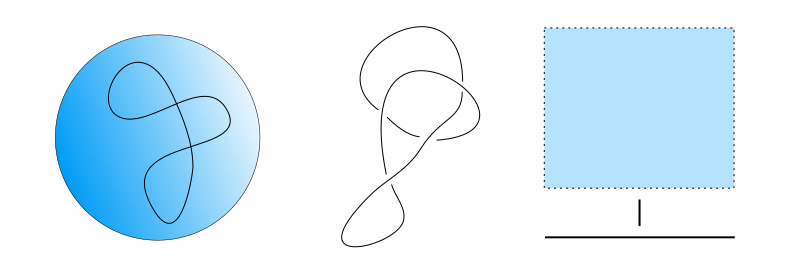
\includegraphics[width=1\textwidth]{reu_figures/immersion_embedding_submersion.png}
    \label{fig:immersion_embedding_submersion}
    \caption{Here are the three types of maps that we have defined: an immersion of a circle on the surface of a blue sphere; an embedding of a circle in 3-d space; and a submersion of an (open) square (as a subset of the plane) into a line segment.}
\end{figure}

\begin{definition} \label{def:isotopies} (Isotopies) Let $X$ and $Y$ be smooth manifolds.
\begin{itemize}
	\item[(a)] An {\bf isotopy} is a map $\Phi:X \times [0,1] \to Y$. We use $\Phi_t:X \to X$ to denote the map $\Phi|_{X \times \{t\}}:X \times \{t\} \to Y$, and we often use the notation $(x,t) \mapsto \Phi_t(x)$ for the isotopy. 
	\item[(b)] An {\bf isotopy of immersions, embeddings or submersions}, respectively, is an isotopy $\Phi:X \times [0,1] \to Y$ where $\Phi_t$ is an immersion, embedding or submersion, respectively, for each $t$.
	\item[(c)] An {\bf ambient isotopy} $\Phi:X \times [0,1] \to X$ is an isotopy such that $\Phi_t$ is a diffeomorphism for each $t$ and $\Phi_0 = \op{Id}$. 
	\item[(d)] The {\bf time derivative} $\frac{d\Phi}{dt}|_s$ at time $s \in [0,1]$ of an isotopy $\Phi:X 
\times [0,1] \to Y$ is the section $\frac{d\Phi}{dt}|_s:X \to \Phi_s^*TY$ given by:
\[
\frac{d\Phi}{dt}|_s := T\Phi(e_t) \circ \iota_s
\]
Let us elaborate on the pieces of this formula.
\begin{itemize}
\item[-] $T\Phi:T(X \times [0,1]) \to \Phi^*TY$ is the tangent space map induced by $\Phi$.
\item[-] $e_t:X \times [0,1] \to T(X \times [0,1])$ is the vector-field on $X \times [0,1]$ pointing in the $t$-direction. More precisely, $e_t$ is the vector-field given by $(x,t) \mapsto (z(x),s(t))$ where we use the identification $T(X \times [0,1) \simeq TX \times T[0,1]$, $z:X \to TX$ is the zero section and $s:[0,1] \to T[0,1] \simeq [0,1] \times \R$ is defined by $s(t) = (t,1)$.

\item[-] $\iota_s:X \to X \times [0,1]$ is the inclusion $x \mapsto (x,s)$ of $X$ into $X \times [0,1]$. 
\item[-] The map $\Gamma(\Phi^*TY) \to \Gamma(\iota_s^*\Phi^*TY) = \Gamma(\Phi_s^*TY)$ that we are using to take $T\Phi$ to $T\Phi \circ \iota_s$ is the map on sections induced by $\iota_s:X \to X \times [0,1$ defined in Definition \ref{def:pullback}(c). We are using the fact that $\Phi_s = \Phi \circ \iota_s$ and thus $\iota_s^*\Phi_s^*TY = (\Phi \circ \iota_s)^*TY = \Phi_s^*TY$, see Proposition \ref{prop:pullback_properties}.
\end{itemize}
\item[(e)] If $Z$ is a vector-field on a manifold $X$, then the {\bf exponential} $\op{exp}_Z:X \times [0,1] \to X$, often denoted by $(x,t) \mapsto \op{exp}(Z)(t,x)$ or $\op{exp}_{tZ}(x)$, is the unique ambient isotopy of $X$ (see Proposition \ref{prop:picard_lindelof}) such that:
\[
\frac{d}{dt}\op{exp}_Z|_s(x) = Z \circ \op{exp}_Z(s,x)
\]
\end{itemize}
\end{definition}

Here are two important existence results about isotopies. The first is a version of a result of Picard-Lindelof, giving an existence result for isotopies with a prescribed time-derivative. The second is called isotopy extension, and it assrts that any isotopy can be factored into a fixed smooth map and an ambient isotopy.

\begin{proposition} \label{prop:picard_lindelof} (Version Of Picard-Lindelof) Let $X$ be a compact manifold with boundary and let $Z:X \times [0,1] \to \pi^*_tTX \subset T(X \times [0,1])$ be a smooth time-dependent vector-field such that $Z|_{[0,1] \times \partial X} = 0$. Then there is a unique ambient isotopy $\Phi:X \times [0,1] \to X$ such that:
\[
\frac{d\Phi}{dt}|_s = Z \circ \Phi_s \qquad \text{and} \qquad \Phi_0 = \op{Id}:X \to X
\]
\end{proposition}

\begin{theorem} (Isotopy Extension Theorem) Let $\Phi:X \times [0,1] \to Y$ be an isotopy of embeddings of a manifold with boundary $X$ through a manifold with boundary $Y$. Assume that there is a neighborhood $U$ of $\partial X$ in $X$ such that $\Phi|_{U \times [0,1]}(x,t) = \Phi_U(x)$ for some smooth $\Phi_U:U \to Y$ where $\Phi_U(\partial X) \subset \partial Y$. 

Then there exists an ambient isotopy $\Psi:Y \times [0,1] \to Y$ such that $\Psi|_{V \times [0,1]}(y,t) = y$ for some neighborhood $V$ of $\partial Y$ and such that $\Phi_t(x) = \Psi_t(\Phi_0(x))$.
\end{theorem}

\begin{motivation} One can think of an isotopy $\Phi:X \times [0,1] \to Y$ as a motion of manifolds that look like $X$ through some ambient space $Y$. Other words that make sense for analogy: a cartoon, a slide show, a flip book etc. 
\end{motivation}

\begin{figure}[h]
    \centering
    \includegraphics[width=1\textwidth]{reu_figures/isotopy.png}
    \label{fig:isotopy}
    \caption{A picture of an isotopy (of embeddings) of $\Phi:S^1 \times [0,1] \to \R^3$. Here we are picturing the isotopy as a series of maps, a cartoon or movie of sorts. The light black outline along with the bold red and blue end circles outline the cylinder $S^1 \times [0,1]$ serving as the domain of the isotopy. The vector-field along the initial red circle is precisely $\frac{d\Phi}{dt}|_0$ as defined in Definition \ref{def:isotopies}(d).}
\end{figure}

The last topic of this section is diffeomorphism and mapping class groups.

\begin{definition} (Diffeomorphisms And Mapping Classes) Let $X$ be a compact manifold with or without boundary. We adopt the following notation and definitions.
\begin{itemize}
\item[(a)] $\op{Diff}(X)$ denotes the group of diffeomorphisms of $X$.
\item[(b)] $\op{Diff}(X,\partial X)$ denotes the group of diffeomorphisms that are the identity on a neighborhood of the boundary. The neighborhood may depend on the particular diffeomorphism.
\item[(c)] $\op{Diff}_0(X) \subset \op{Diff}(X)$ denotes the subgroup of diffeomorphisms $\varphi$ that are isotopic to the identity through diffeomorphisms, i.e. such that there exists an ambient isotopy $\Phi:X \times [0,1] \to X$ such that $\Phi_1 = \varphi$.
\item[(d)] $\op{Diff}_0(X,\partial X) \subset \op{Diff}(X,\partial X)$ denotes the subgroup of diffeomorphisms $\varphi$ in $\op{Diff}(X,\partial X)$ that are isotopic to the identity through diffeomorphisms in $\op{Diff}(X,\partial X)$, i.e. such that there exists an ambient isotopy $\Phi:X \times [0,1] \to X$ such that $\Phi_1 = \varphi$ and such that $\Phi_t$ is the identity in a neighborhood of $\partial X$ for each $t$.
\item[(e)] The {\bf mapping class group} $\op{MC}(X)$ of $X$ is defined to be the quotient group $\op{Diff}(X)/\op{Diff}_0(X)$. An element $[\varphi] \in \op{MC}(X)$ is called a {\bf mapping class}.
\item[(f)] The {\bf mapping class group rel boundary} $\op{MC}(X,\partial X)$ of $(X,\partial X)$ is defined to be the quotient group $\op{Diff}(X,\partial X)/\op{Diff}_0(X,\partial X)$. An element $[\varphi] \in \op{MC}(X,\partial X)$ is also called a {\bf mapping class}.
\end{itemize}
\end{definition}

\begin{motivation} (Mapping Classes) If one thinks of isotopies of diffeomorphisms as being ``paths in the space of diffeomorphisms,'' then one can think of $\op{MC}(X,\partial X)$ as a being the set of connected components of 
\end{motivation}

\begin{exercise} Here are some exercises about maps of manifolds.
\begin{enumerate}
	\item[(a)] (Courtesy Of Nikhil) Find an example of an injective immersion $f:X \to Y$ that is not an embedding. Find two injective immersions $f_1:X_1 \to Y$ and $f_2:X_2 \to Y$ with the same image $f_1(X_1) = f_2(X_2)$ but where $X_1$ and $X_2$ are not homeomorphic. (Hint: Here's a possibility. Let $Y = \R^2$ and try to make $f_1(X_1)$ and $f_2(X_2)$ shaped like a $\phi$.)
	\item[(b)] Let $I = [0,1]$ be the interval and $\partial I = \{0,1\}$. Show that $\op{MC}(I,\partial I)$ is the trivial group. That is, show that, for any smooth and smoothly invertible map $f:[0,1] \to [0,1]$, there exists a smooth map $g:[0,1] \times [0,1] \to [0,1]$, $(t,x) \mapsto g_t(x)$, such that $g_1(x) = f(x)$, $g_0(x) = x$ and $g_t:[0,1] \to [0,1]$ is smooth and smoothly invertible for every $t \in [0,1]$.  
	\item[(c)] (Hard) Let $A = S^1 \times [0,1]$ be the annulus, whose boundary is $\partial A = S^1 \sqcup S^1$. Here we will identity $S^1$ as the unit circle in $\C$. Prove that $\op{MC}(A,\partial A) \simeq \Z$.
\end{enumerate}
\end{exercise}

\subsection{Constructing Manifolds} In this section, we will discuss several ways of constructing new manifolds from old ones. We first discuss the simplest examples, where the atlas structure is obvious. We then discuss fibers of submersions, which have a natural manifold structure. This is a consequence of, and can be interpreted as a generalization of, the Implicit Function Theorem (see Appendix \ref{subsec:inverse_and_implicit}). Finally, we discuss gluing manifolds with boundary along components of said boundary. This construction has many important special cases: connect sums, mapping tori and open books are the ones that we will discuss.

\begin{proposition} \label{prop:constructions_of_manifolds} (Basic Constructions) We will now discuss the most elementary constructions of new manifolds from old. 
\begin{enumerate} 
	\item[(a)] (Open Subsets): Any open subset $U \subset M$ of a manifold $M$ is itself a manifold. 
	\item[(b)] (Disjoint Unions): The disjoint union $M \sqcup N$ of two manifolds is a manifold.
	\item[(c)] (Products): The product $M \times N$ of two manifolds is a manifold.
	\item[(d)] (Pullback): Given a smooth manifold $M$, a topological space $X$ and a homeomorphism $\varphi:X \simeq M$, $X$ has a canonical smooth structure that makes $\varphi$ a diffeomorphism:
\end{enumerate}
\end{proposition}

\begin{proof} We will now define an atlas for each of these examples. By Remark \ref{rmk:def:manifold}, the atlas that we define doesn't need to be maximal. In each of these cases, checking the atlas axioms is trivial.

\vspace{5pt}

\emph{(a) - Open Subsets:} If $\mathcal{A}$ is the atlas of $M$, then the atlas $\mathcal{B}$ of $U$ consists of charts $(V \cap U, \varphi|_{U \cap V})$ where $(V,\varphi)$ is a chart in $\mathcal{A}$.

\vspace{5pt}

\emph{(b) - Disjoint Unions:} The disjoint union atlas $\mathcal{A} \sqcup \mathcal{B}$ is just the union of the atlases $\mathcal{A}$ and $\mathcal{B}$.  

\vspace{5pt} 

\emph{(c) - Products:} The product atlas $\mathcal{A} \times \mathcal{B}$ is just the set of charts $(U \times V,\varphi \times \psi)$ for $(U,\varphi) \in \mathcal{A}$ and $(V,\psi) \in \mathcal{B}$.

\vspace{5pt}

\emph{(d) - Pullback:} Here we just take the atlas $\varphi^*\mathcal{A}$ on $X$ to be the set:
\[
\varphi^*\mathcal{A} = \{(\varphi^{-1}(U),\phi \circ \varphi| (U,\phi) \in \mathcal{A}\}
\] \end{proof}

Another extremely common way of producing manifolds is as fibers of submersions. The following result codifies this method. 

\begin{proposition} (Fibers Of Submersions) Let $f:X \to Y$ be a smooth map and fix $y \in Y$. Suppose that $f$ is a submersion along $f^{-1}(y)$: that is, for every $x \in f^{-1}(y)$, $T_xf:T_xX \to f^*T_yY$ is surjective. Then:
\begin{itemize}
\item{(a)} (Manifold Structure) $F = f^{-1}(y) \subset X$ has a natural manifold structure.
\item{(b)} (Embedded) The inclusion $\iota:F \to X$ is an embedding.
\end{itemize}
\end{proposition}

\begin{proof} \emph{(a) - Manifold Structure:} We define an atlas $\mathcal{F}$ on $F$ like so. Take any $x \in F$ and any pair of charts $(U,\varphi)$ on $X$ and $(V,\psi)$ on $Y$ such that $f(x) = y$ is in $V$. Then the map:
\[\psi \circ f \circ \varphi^{-1}:\varphi(U \cap f^{-1}(V)) \to \psi(V)\]
is a smooth map between (non-empty) open subsets of $\R^{m + n}$ and $\R^m$. 

Denote $g = \psi \circ f \circ \varphi^{-1}$, $P = \varphi(U \cap f^{-1}(V)) \subset \R^{m+n}$ and $Q = \psi(V) \subset \R^n$. Also denote $\op{dim}(X) = m + n$ and  $\op{dim}(Y) = m$. Note that $T_xf$ is surjective, $T_z\psi_z$ and $T_p\varphi^{-1}$ are isomorphisms for any points $p \in P$ and $z \in V$. Thus the map:
\[dg_{\varphi(x)}:\R^{m + n} = T_{\varphi(x)}P \to T_{g(\varphi(x))}Q = \R^m\]
is surjective, since by the composition property of $Tg$ we have the equation:
\[dg_{\varphi(x)} = T_{\varphi(x)}g = T_{f(x)}\psi \circ T_xf \circ T_{\varphi(x)}\varphi^{-1}\]
 The surjectivity of the linear map $dg_{\varphi(x)}$ implies that we can pick a splitting $\R^{m+n} \simeq \R^{m} \oplus \R^{n}$ so that $dg_{\varphi(x)}|_{\R^m}:\R^m \oplus \{0\} \simeq \R^m$ is an isomorphism. Thus by the Implicit Function Theorem \ref{thm:implicit_function_theorem}, we can choose a neighborhood $A \subset \R^n \oplus \R^m$, a neighborhood $B \subset \R^{m+n}$ of $\varphi(x)$ and a diffeomorphism $g:A \simeq B$ such that $g((\R^n \oplus 0) \cap A) = B \cap \varphi(F)$. With this set of choices, we can define a chart $(O,\phi)$ on $F$ by:
\[
O := \varphi^{-1}(B \cap \varphi(F)) \qquad \phi := \pi_{\R^n} \circ g^{-1} \circ \varphi|_O
\]
Here $\pi_{\R^n}:\R^n \oplus \R^m \to \R^n$ is projection to the $\R^n$ component. Note that the inverse of $\phi$ is given (in terms of the inclusion $\iota_{\R^n}:\R^n \to \R^n \oplus \R^m$) as:
\[
\phi^{-1} = \varphi^{-1} \circ g \circ \iota_{\R^n}
\]

 We now define the atlas $\mathcal{F}$ on $F$ to be the set of all charts $(O,\phi)$ constructed as above. To check the atlas axioms, we note first that the covering axiom is immediate: we perform this construction for every $x \in F$. For the transition axioms, we note that if $(O_0,\phi_0)$ and $(O_1,\phi_1)$ are two charts in $\mathcal{F}$, then on the domain of definition the transition map is given by:
 \[
 \phi_1 \circ \phi_0^{-1} = \pi_{\mathbb{R}^n} \circ (g_1^{-1} \circ \varphi_1 \circ \varphi_0^{-1} \circ g_0) \circ \iota_{\R^n}
 \]
 The middle expression is a diffeomorphism between open subsets of $\R^n \oplus \R^m$, and thus the whole expression is smooth between the appropriate open subsets of $\R^n$.

\emph{(b) - Embedded:} To check that the map $\iota:F \to X$ is an embedding, we just need to check that the map $\iota \circ \phi^{-1}$ is an immersion for any chart $(O,\phi)$ on $F$. Indeed, the definition of the chart maps show that on their domain of definition $\iota \circ \phi^{-1} = \varphi^{-1} \circ g \circ \iota_{\R^n}$ where $\varphi^{-1} \circ g$ is a diffeomorphism and $\iota_{\R^n}$ is an immersion. It follows that $\iota \circ \phi^{-1}$ is an immersion. \end{proof}

In the proof of Proposition \ref{prop:constructions_of_manifolds}, we utilized the implicit function theorem, itself a consequence of the inverse function theorem. These results are discussed in Appendix \ref{subsec:inverse_and_implicit}.

The last few construction methods that we will discuss here are all instances of instances of a construction that we will term ``boundary gluing'' in these notes. The idea is that if a single manifold has two boundary components that are diffeomorphic (or if two manifolds have diffeomorphic boundaries) we can glue the two boundary components together to close up the original manifold in that area, creating a new manifold. Here is a result formalizing the above idea.

\begin{proposition} \label{prop:boundary_gluing} (Boundary Gluing) Let $X$ be a manifold with boundary. Let $C,D \subset \partial X$ be closed components of $\partial X$ respectively, and let $\varphi:C \simeq D$ be a diffeomorphism. Consider the equivalence relation $\sim_\varphi$ on $X$ given by:
\[
x \sim_\varphi y \text{ if }\left\{
\begin{array}{cc}
y = \varphi(x) & \text{ if }x \in C, y \in D\\
x = \varphi(y) & \text{ if }x \in D, y \in C\\
\end{array}\right.
\]
Then $X/\sim_\varphi$ is there exists a natural smooth structure on $X/\sim_\varphi$. If $\phi:C \to D$ and $\psi:C \to D$ are isotopic through diffeomorphisms, then $X/\sim_\phi \simeq X/\sim_\psi$.
\end{proposition}

\begin{proof} Consider $X \sqcup C \times (-1,1)$ and pick tubular neighorhoods $\tau_C:C \times (-1,0] \to X$ and $\tau_D:D \times [0,1) \to X$ of $C$ and $D$ respectively. Let $\tau = (\tau_C,\tau_D)$ denote the choice of this pair of tubular neighborhoods, and let $\widetilde{X}_{\tau,\phi}$ denote the quotient of $X \sqcup C \times (-1,1)$ by the equivalence relation generated by:
\[(x,s) \sim \tau_C(x,s) \text{ for }(x,s) \in C \times (-1,0]\]
\[ (x,s) \sim \tau_D(\varphi(x),s) \text{ for }(x,s) \in C \times [0,1)\]
Furthermore let $\pi:X \sqcup C \times (-1,1) \to \widetilde{X}_{\tau,\phi}$ be the quotient map. An atlas on $\widetilde{X}_{\tau,\phi}$ can be defined as:
\[
\widetilde{\mathcal{A}} = \{(\pi(U),\phi \circ \pi|_{\pi(U)}^{-1})| (U,\phi) \text{ is a chart on }(X \setminus (C \sqcup D)) \sqcup C \times (-1,1)\}
\]
The atlas axioms follow from those on $(X \setminus (C \sqcup D)) \sqcup C \times (-1,1)$. There is a homeomorphism $[\iota]_\tau:X/\sim_\varphi \simeq \widetilde{X}_{\tau,\phi}$ descending from the inclusion $\iota:X \to X \sqcup C \times (-1,1)$, and we define the smooth structure on $\widetilde{X}_{\tau,\phi}$ to be $[\iota]^*_\tau\widetilde{A}$. The construction of $\widetilde{X}_{\tau,\phi}$ depends on a choice of tubular neighborhood data $\tau$, but it is simple to verify that the map $[\iota]_{\tau} \circ [\iota]_{\sigma}^{-1}:\widetilde{X}_{\sigma,\varphi} \to \widetilde{X}_{\tau,\varphi}$ is a diffeomorphism for two choices $\sigma$ and $\tau$ of tubular neighborhood data, so that the smooth structure $[\iota]_\tau^*\widetilde{A}$ is independent of $\tau$.
\end{proof}

We now discuss various special cases of the above construction. These include connect sums, mappin tori and open books. 

\begin{definition} (Connect Sums) Let $X$ and $Y$ be two connected, compact $n$-manifolds. We define the connect sum $X \# Y$ as so. Let $\iota_X:B^n \to X$ and $\iota_Y:B^n \to Y$ be embeddings of the closed $n$-ball into $X$ and $Y$ respectively. Then the manifold:
\[Z := X \sqcup Y \setminus \iota_X(\op{int}(B^n)) \sqcup \iota_Y(\op{int}(B^n))\]
has two $S^{n-1}$ boundary components $C$ and $D$, one from the boundary of the ball embedded into $X$ and one from the boundary of the ball embedded into $Y$. Pick an arbitrary diffeomorphism $\varphi:C \simeq D$ and, using Proposition \ref{prop:boundary_gluing}, define:
\[
X \# Y := Z/\sim_{\varphi}
\] 
\end{definition}

\begin{lemma} The connect sum is independent of the choice of $\iota_X,\iota_Y$ and $\varphi$ in the sense that any two choices of such data yield diffeomorphic manifolds.
\end{lemma}

\begin{proof} (Sketch) It suffices to show that any two embeddings $\iota_0,\iota_1:B^n \to X$ where ($X$ is connected) are isotopic in the sense that there exists an ambient isotopy $\Phi:X \times [0,1] \to X$ such that $\iota_1 = \Phi \circ \iota_0$. 

 To see this, look at the centers $\iota_0(0), \iota_1(0)$ of the balls in $X$. The centers are connected by a path $\gamma:[0,1] \to X$. By the isotopy extension theorem, we can find an isotopy $\Phi:[0,1] \times X \to X$ such that $\Phi_i(0) = \gamma(i) = \iota_i(0)$. Thus we can assume that $\iota_0(0) = \iota_1(0)$. 

 Then we show that we can assume that $\iota_0(B^n) \subset \op{int}(\iota_1(B^n))$. We can do this by constructing a vector-field $v$ on $X$ which looks like the radial vector-field when restricted to $\iota_0(B^n)$, and then applying Picard-Lindelof to get a flow which contracts $\iota_0(B^n)$ to a small neighborhood of $\iota_0(0)$. 

 Finally, we have reduced to the case of showing that any embedding $\iota:B^n \to \op{int}(B^n) \subset B^n$ where $\iota(0) = 0$ is isotopic to the identity map $B^n \to B^n$. This is an excellent exercise, which the reader is welcome to do. We will fill in this part of the sketch if we have time. 
\end{proof}

\begin{definition} (Mapping Torus) Let $X$ be a compact smooth manifold with boundary and let $\varphi:X \to X$ be a diffeomorphism. Then the {\bf mapping torus} $M(X,\varphi)$ is the quotient space:
\[
\op{Map}(X,\varphi) = X \times [0,1]/\sim_\varphi
\]
Where here we identify the two boundary components $X \times \{0\}$ and $X \times \{1\}$ by the equivalence relation $\sim_\varphi$ defined by:
\[
(\varphi(x),0) \sim_\varphi (x,1)
\]
\end{definition}

\begin{definition} (Open Books) An {\bf abstract open book} $(P,\phi)$ is a pair of a smooth manifold with boundary $P$ and a diffeomorphism $\phi:P \to P$ that is the identity in a neighborhood of the boundary. The manifold $P$ is called the {\bf page}, the boundary $\partial P$ is called the {\bf binding} and the map $\phi:P \to P$ is called the {\bf page map} or {\bf monodromy}.

The {\bf geometric open book} or {\bf geometric realization} $B(P,\phi)$ of an abstract open $(P,\phi)$ is the manifold constructed as so. Let $\op{Map}(P,\phi)$ be the mapping torus of $(P,\phi)$. Then the boundary $\partial \op{Map}(P,\phi)$ is canonically diffeomorphic to $\partial P \times S^1$. Similarly, the boundary $\partial (\partial P \times D^2)$ of the manifold $\partial P \times D^2$ (given by crossing $\partial P$ with the $2$-disk) is also canonically identified with $\partial P \times S^1$. Thus we have a diffeomorphism $\varphi:\partial \op{Map}(P,\phi) \simeq \partial (\partial P \times D^2)$ and we can form the quotient:
\[
B(P,\phi) := \op{Map}(P,\phi) \sqcup \partial P \times D^2 /\sim_{\varphi}
\]

An {\bf open book decomposition} of a manifold $X$ is an abstract open book $(\Sigma,\phi)$ and a diffeomorphism $X \simeq B(P,\phi)$.
\end{definition}

\begin{lemma} The diffeomorphism type of $B(P,\phi)$ depends only on the mapping class $[\phi] \in \op{MC}(P,\partial P)$.
\end{lemma}

\begin{exercise} Here are some exercises regarding these constructions.
\begin{itemize}
	\item[(a)] Show that the only $2$-manifolds with open book decompositions where the pages are compact with non-trivial boundary are disojoint unions of $2$-spheres.
	\item[(b)] Show that the geometric open book $B(B^n,\op{Id})$ of the abstract open book $(B^n,\op{Id})$, with page the $n$-ball $B^n$ and monodromy map given by the identity $\op{Id}:B^n \to B^n$, is diffeomorphic to the $(n+1)$-sphere.
	\item[(c)] Let $A = S^1 \times [0,1]$ and let $\tau:A \to A$ be the map $(\theta,t) \mapsto (\theta + t,t)$. This map is called the {\bf dehn twist} of $S^1 \simeq [0,1]$. Show that the geometric open book $B(A,\tau)$ is the $3$-sphere.
	\item[(d)] (Very Hard) Let $DS^n$ denote the unit disk bundle of the tangent bundle of the sphere with respect to some metric. Find a mapping class $[\tau] \in \op{MC}(DS^n,\partial DS^n)$ where the open book $(DS^n,\tau)$ has $B(DS^n,\tau) \simeq S^{2n+1}$.
\end{itemize}
\end{exercise} 

\subsection{Pullback, Lie Derivatives, Exterior Derivatives And Integration} \label{subsec:exterior_calculus} There are several fundamental operations on differential forms that show up constantly when one is performing calculations. Some of these operations are inherited from the fiberwise structure of the alternating algebra: the wedge product and interior product are examples of this fiberwise structure. There are others, however, that only make sense at the level of sections: pullbacks, Lie derivatives, exterior derivatives and integration are the prime examples. 

In this section, \S \ref{subsec:exterior_calculus}, we will define these global operations, give some intuition and discuss their key properties.

\begin{definition} \label{def:form_pullback} (Pullback)  Let $f:X \to Y$ be a smooth map. The {\bf pullback map} $f^*:\Omega(Y) \to \Omega(X)$ of $k$-forms on $Y$ to $k$-forms on $X$ is defined on a section $\omega \in \Omega(X)$ as:
	\[
	f^*\omega = \Lambda(T^*f)(\omega \circ f)
	\]
Recall where we defined the maps in this definition.
\begin{itemize}
\item[-] $\omega \circ f = \Gamma(f)\omega$ is the section of the pullback $f^*\Lambda^kX$ gotten by applying the map $\Gamma(f):\Gamma(\Lambda Y) \to \Gamma(f^*\Lambda Y)$ (described in Proposition \ref{prop:pullback_properties}) to $\omega$.
\item[-] $\Lambda(T^*f):f^*\Lambda(T^*Y) \to \Lambda(T^*X)$ is the bundle map $f^*\Lambda(T^*Y) = \Lambda(f^*T^*Y) \to \Lambda(T^*X)$ induced by the map $T^*f:f^*T^*Y \to T^*X$ described in Definition \ref{def:bundles_on_smooth_manifolds}(2)(b) for the cotangent bundle. 
\end{itemize}
\end{definition}

\begin{proposition} The pullback map $f^*:\Omega(X) \to \Omega(X)$ is a map of algebras: it is linear and it commutes with the wedge product.
\end{proposition}

\begin{remark} \label{rmk:def:form_pullback} This definition can seem a little opaque, but we can write a fiberwise expression for $f^*\omega$ using the discussion in Review \ref{rev:exterior_algebra}(d) about the relationship between anti-symmetric multi-linear forms and the exterior algebra. 

Recall that any element $\omega_y \in \Lambda^k(T^*Y)_y$ at a point $y \in Y$ can be viewed a $k$-linear form $\omega_y:\times_1^k T_yY \to \mathbb{R}$ by the discussion in Review \ref{rev:exterior_algebra}(d). We denote this by $(v_1,\dots,v_k) \mapsto \omega_y(v_1,\dots,v_k) \in \R$. Thus, given a section $\omega \in \Omega^k(Y)$ of $\Lambda^kY = \Lambda^k(T^*Y)$, we get a $k$-linear function $\omega_y$ on $T_yY$ at each point $y \in Y$. Similarly, given a map $f:X \to Y$, we can pull back to get a section $f^*\omega$ of $\Omega^k(X)$ and thus a $k$-linear function $f^*\omega_x$ at each $x \in X$. 

In these terms, we can write $f^*\omega_x$ as:
\[
f^*\omega_x(u_1,\dots,u_k) = \omega_{f(x)}(Tf(u_1),\dots,Tf(u_k))
\]
In words, this says the following: to evaluate $f^*\omega_x$ on some vectors $u_1,\dots,u_k \in T_xX$, we first push each $u_i$ through the map $Tf:TX \to f^*TY$ to get a vector $Tf(u_i) \in f^*TY_x = TY_{f(x)}$. Then we evaluate $\omega_{f(x)}:\times_1^k T_{f(q)}Y \to \R$ on the tuple $(Tf(u_1),\dots,Tf(u_k))$. This gives us the desired quantity. 

\end{remark}

\begin{motivation} Remark \ref{rmk:def:manifold} along with Motivation \ref{mot:exterior_algebra} combine to give the following motivation for what the pullback is doing. In a small neighborhood $U$ of a point $x \in X$, the space $X$ looks very much like $T_xX$ and $f$ looks very much like the map $Tf:T_xX \to T_{f(x)}Y$. We can think of a very small $k$-dimensional parallelepid $P(u) = M(u)C \subset T_xX$ where $M(u) = [u_1|\dots|u_k]$ with $u_i \in T_xX$ and $C$ is the unit cube. When we take $f(P(u))$ (which looks very much like $Tf(P(u))$) we can ask what the area is with respect to $\omega$. Our answer comes from the pullback.
\begin{center}
\emph{If $P(u)$ is a very very small parallelepipid near $x \in X$, we can take $f(P(u))$ and ask what ``area'' this $k$-dimensional object has with respect to a $k$-form $\omega$ near $f(x)$. The answer is approximately $f^*\omega_x(u_1,\dots,u_k)$ up to a very small error.}
\end{center}
\end{motivation}

\begin{figure}[h]
    \centering
    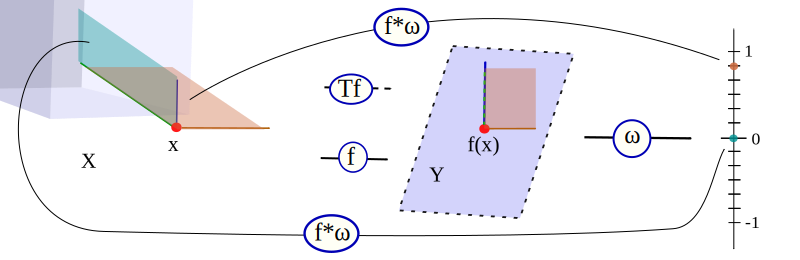
\includegraphics[width=1\textwidth]{reu_figures/pullback_of_form.png}
    \label{fig:form_pullback}
    \caption{A diagram explaining Remark \ref{rmk:def:form_pullback}. Here we have a 3-manifold $X$ (on the right) and a $2$-manifold $Y$, along with a map $f:X \to Y$ and a $2$-form $\omega$ on $Y$. The point $x \in X$ maps to $f(x) \in Y$, and there is an induced map of tangent spaces $Tf:T_xX \to T_{f(x)}Y$. To get the value of $f^*\omega_x$ on the blue and green vectors $u_g,u_b \in T_xX$, we simply apply the $Tf$ map to these two vectors and then evaluate $\omega_{f(x)}$ on the result. This is what is occuring in the picture. Note that the green and blue vectors get sent to the same place, so the plane that they span is degenerate and thus $f^*\omega$ evaluates to $0$ on the pair.}
\end{figure}

\begin{definition} \label{def:exterior_derivative} (Exterior Derivative) The exterior derivative $d:\Omega(X) \to \Omega(X)$ is the unique map satisfying the following axioms.
\begin{itemize}
	\item[(a)] (Linearity) If $\alpha,\beta \in \Omega(X)$ and $c \in \R$, then:
	\[d(c\alpha) = c(d\alpha) \qquad d(\alpha + \beta) = d\alpha + d\beta\]
	\item[(b)] (0-Forms) If $f \in \Omega^0(X)$ then $df$ is defined as so. A map smooth $f:X \to \R$ induces a bundle map $Tf:TX \to f^*T\R \simeq X \times \R$. This map is the same as a section of $\op{Hom}(TX,\R) = T^*X$. $df$ is defined to be this section.
	\item[(c)] (Leibniz Rule) If $\alpha \in \Omega^j(X)$ and $\beta \in \Omega^k(X)$, then:
	\[d(\alpha \wedge \beta) = d\alpha \wedge \beta + (-1)^j \alpha \wedge d\beta\]
\end{itemize}
Note that $d(\Omega^k(X)) \subset \Omega^{k+1}(X)$, that is $d$ increases the degree of a form by $1$.
\end{definition}

The exterior derivative can be thought of in many ways. It provides a natural co-chain complex structure to the differential forms, yielding a version of manifold homology (see \S \ref{subsec:de_rham_cohomology}). Relatedly, one can think of the exterior derivative as being the adjoint to the boundary map via the integration pairing via Stokes theorem (see Theorem \ref{thm:stokes}).

\begin{definition} \label{def:lie_derivative} (Lie Derivative) The Lie derivative $\mathcal{L}:\Gamma(TX) \times \Omega(X) \to \Omega(X)$ is the unique map satisfying the following axioms.
\begin{itemize}
	\item[(a)] (Linearity) if $\alpha,\beta \in \Omega(X)$, $u,v \in \Gamma(TX)$ and $c \in \R$, then:
	\[\mathcal{L}_{u + v}\alpha = \mathcal{L}_u\alpha +  \mathcal{L}_v\alpha \qquad \mathcal{L}_v(\alpha + \beta) = \mathcal{L}_v\alpha + \mathcal{L}_v\beta \qquad \mathcal{L}_{cv}\alpha = \mathcal{L}_v(c\alpha) = c\mathcal{L}_v\alpha\]
	\item[(b)] (0-Forms) If $f \in \Omega^0(X)$ and $v \in \Gamma(TX)$ then $\mathcal{L}_vf = \iota_v df$ or $\mathcal{L}_vf = df(v)$.
	\item[(c)] (Leibniz Rule) If $\alpha,\beta \in \Omega(X)$ and $v \in \Gamma(TX)$ then:
	\[\mathcal{L}_v(\alpha \wedge \beta) = \mathcal{L}_v\alpha \wedge \beta + \alpha \wedge \mathcal{L}_v\beta\]
	\item[(d)] (Exterior Derivative) $d$ and $\mathcal{L}$ commute, in the snese that for any $v \in \Gamma(TX)$ and any $\omega \in \Omega(X)$:
	\[
	d(\mathcal{L}_v\omega) = \mathcal{L}_v(d\omega)
	\] 
\end{itemize}
Note that, for any vector-field $v$, $\mathcal{L}_v(\Omega^k(X)) \subset \Omega^k(X)$, so the Lie derivative preserves the degree of any differential form.
\end{definition}

The Lie derivative $\mathcal{L}_v\omega$ with respect to a vector-field $v$ is best understood using (what we are calling) the fundamental identity of the Lie derivative. 

\begin{proposition} Let $X$ be a compact manifold, let $v \in \Gamma(TX)$ be a vector-field, let $\omega \in \Omega(X)$ be a differential form and let $\Phi_t:X \times [0,\epsilon) \to X$ be any ambient isotopy satisfying $\frac{d}{dt}(\Phi_t)|_{t = 0} = v$. The following are equal.
\begin{itemize}
	\item[(a)] (Algebraic Lie Derivative) The Lie derivative $\mathcal{L}_v\omega$ of Definition \ref{def:lie_derivative}.
	\item[(b)] (Infinitesimal Pullback) The time-derivative $\frac{d}{dt}(\Phi^*_t\omega)|_{t = 0}$ of the time-dependent family of differential forms $\Phi^*_t\omega$.
	\item[(c)] (Cartan's Magic Formula) The anti-commutator of interior product and exterior derivative: $d(\iota_v\omega) + \iota_v(d\omega)$.
\end{itemize}
\end{proposition}

\begin{proof} Verify that (b) and (c) above both satisfy Properties (a)-(d) in Definition \ref{def:lie_derivative}. The result then follows from the fact that the Lie derivative is uniquely characterized by these properties.
\end{proof}

Our last topic of discussion in this chapter will be integration. 

\begin{definition} \label{def:integration} (Integration) Let $X = (X,o)$ be a compact oriented $n$-manifold with boundary and let $\mu \in \Omega^n(X)$ be an $n$-form on $X$. We define the integral $\int_X \mu$ as so.

First, consider any $\mu \in \Omega^n(\R^n)$ such that $\mu$ is $0$ outside of a compact subset of $\R^n$. The exterior derivatives $\{dx_i\}_{i=1}^n$ form a basis of the cotangent space $T^*_p\R^n$ at each point $p \in \R^n$, and thus $dx_1 \wedge \dots \wedge dx_n$ spans (point-wise) the fiber of $\Lambda^n_p\R^n$. It follows that any $\mu$ can be written as $\mu = f dx_1 \wedge \dots \wedge dx_n$ for some smooth $f:\R^n \to \R$. Note that $f$ must also be $0$ outside of a compact subset of $\R^n$. Thus we define the integral of $\mu$ to be the integral of $f$, i.e:
\[
\int_{\R^n} \mu = \int_{\R^n} f dx_1 \wedge \dots \wedge dx_n := \int_{\R^n} f dx_1 \dots dx_n
\]

Pick any finite open cover $\{U_i\}_{i=1}^n$ of charts $(U_i,\varphi_i)$ on $X$ such that $\varphi_i^*o_{\mathbb{R}^n} = o$. Here $o_{\R^n} = [dx_1 \wedge \dots \wedge dx_n]$ is the canonical orientation on $\R^n$. Pick a partition of unity $\{\psi_i\}$ on $X$ supported on $U_i$: this is, by definition, a set of smooth maps $\psi_i:X \to \R$ such that:
\begin{itemize}
\item[(a)] $\psi_i$ is $0$ away from a compact subset of $U_i$.
\item[(b)] $0 \le \psi_i(x) \le 1$ for any $x \in X$.
\item[(c)] $\sum_i \psi_i(x) = 1$ for any $x \in X$.
\end{itemize}
Then we define the integral of $\mu$ over $X$ to be:
\[
\int_X \mu := \sum_i \int_{\R^n} (\varphi_i^{-1})^*(\psi_i \cdot \mu)
\]
\end{definition}

\begin{proposition} \label{prop:integral_well_definedness} The integral $\int_X \mu$ depends only on $X$, $o$ and $\mu$, and not on the choices of $U_i, \varphi_i$ or $\psi_i$.
\end{proposition}

\begin{motivation} To give the reader some idea of why Proposition \ref{prop:integral_well_definedness} is true, we consider the following. Let $\mu \in \Omega^n(\R^n)$ be an $n$-form that is $0$ outside of a compact set and let $\varphi:\R^n \to \R^n$ be a diffeomorphism preserving the standard orientation $o_{\R^n}$, with $\varphi(x) = (\varphi^i(x))_{i=1}^n$ ($\varphi^i$ are the component functions) and $\varphi^i(x) = y_i$ being the new coordinates. 

We know that $\mu = f dy_1 \wedge dy_n$ for a smooth function $f:\R^n \to \R$. If we compute the integral of $\mu$ in the $x$ coordinates inst{}ead of the $y$ coordinates, we see that:
\[
\int_{\R^n} \mu = int_{\R^n} f(y_1,\dots,y_n) dy_1\dots dy_n = \int_{\R^n} f(\varphi^1(x),\dots,\varphi^n(x)) |\op{det}(d\varphi)| dx_1 \dots dx_n\]
\[= \int_{\R^n} \varphi^*f \cdot |\op{det}(d\varphi)| dx_1 \wedge \dots \wedge dx_n  = \int_{\R^n} \varphi^*f \cdot \varphi^*(dy_1 \wedge \dots \wedge dy_n) = \int_{\R^n} \varphi^*\mu
\]
Here we use the following facts. First, the change of coordinates formula for an integral. Second, the fact that for an orientation preserving diffeomorphism $\R^n \to \R^n$, the determinant $\op{det}(d\varphi)$ is positive and thus equal to its absolute value. Third, the fact that:
\[\varphi^*(dx_1 \wedge \dots dx_n) = \op{det}(d\varphi) \cdot dy_1 \wedge \dots dy_n\]
This is related to Exercise \ref{ex:linear_algebra}(c). Fourth, we use the fact that $\varphi^*\alpha \wedge \varphi^*\beta = \varphi^*(\alpha \wedge \beta)$ (if $\alpha$ is a function, this just reduces to multiplication). 

The above discussion essentially shows that different choices of chart map $\varphi_i$ in Definition \ref{def:integration} do not effect the integral. 
\end{motivation}

The key result about integration on manifolds is the following.

\begin{theorem} \label{thm:stokes} (Stokes Theorem) Let $X = (X,o_X)$ be an oriented $n$-manifold. Let $\partial X = (\partial X,o_{\partial X})$ be the boundary, oriented with the boundary orientation $o_{\partial X}$, and let $\iota:\partial X \to X$ denote inclusion. Finally, let $\omega \in \Omega^{n-1}(X)$ be an $(n-1)$-form. Then: 
\[
\int_{\partial X} \iota^*\omega = \int_X d\omega
\]
\end{theorem}

\section{Manifold Homology} \label{sec:manifold_homology} This section will be an introduction to homology. Homology theory in its various incarnations is one of the most fundamental tools in modern topology. It possesses a unique combination of simplicity, usefulness and ubiquity that is difficult to appreciate when one first learns about it. We will only be scratching the surface in these notes.

Here is how this section is organized. In \S \ref{subsec:what_is_homology}, we will introduce the algebraic definition of homology and cohomology, and we give the motivation for where these algebraic properties come from. In \S \ref{subsec:singular_homology}-\ref{subsec:de_rham_cohomology}, we give several examples of homology theories: singular homology in \S \ref{subsec:singular_homology}, simplicial homology in \S \ref{subsec:simplicial_homology} and de Rham cohomology in \S \ref{subsec:de_rham_cohomology}. In these sub-sections, we will also discuss the relationships between these theories.

\subsection{What Is Homology?} \label{subsec:what_is_homology} At the most basic level, homology is a straight forward algebraic construction. Before we state the definition for this construction, we give a motivational ``derivation'' of the properties of chain complexes and their homology groups.

\begin{motivation} \label{mot:groups_of_sub_manifolds} (Groups Of Sub-Manifolds) Let $X$ be a manifold. We will now describe an informal construction of homology. {\bf Warning:} The contents of this section are very non-rigorous. They should be used purely for conceptual aid.

We want to understand $X$ by extracting quantitative information from it. That means we want to calculate some numerical or algebraic invariant from $X$, something that is essentially determined by the isomorphism class (i.e., diffeomorphism type) of $X$, but preferably something that isn't trivial. One way of understanding an object is to understand maps into or out of the object. This is sort of a mathematical meta-principle; it applies in a multitude of contexts. In our case, we can try to understand the collection $\op{Map}(-,X)$ of pairs $(\Sigma,\iota)$ where $\Sigma$ is a connected, compact manifold with boundary and $\iota:\Sigma \to X$ is a smooth map\footnote{The collection of pairs $(\Sigma,\iota)$ of a compact manifold with boundary $\Sigma$ and a map $\iota:\Sigma \to X$ is very much not a set. There is a ``set of sets'' problem here. This is immaterial for motivational purposes.}. 

We can build an algebraic object out of $\op{Map}(-,X)$ in a naive way by making a ``chain group'' generated by all of the objects in $\op{Map}(-,X)$.
\[
C(X;\mathbb{F}_2) = \mathbb{F}_2 \cdot \op{Map}(-,X)
\]
Here $\mathbb{F}_2 = \Z/2\Z$ is the field of $2$ elements and $\mathbb{F}_2 \cdot \op{Map}(-,X)$ denotes the group of formal linear combinations of finitely many elements of $\op{Map}(-,X)$ with coefficients in $\mathbb{F}_2$. Now we have an algebraic object, but it is much to big to be useful: it would be ideal if our construction produced a group that was finite in some sense, perhaps finitely generated or even literally finite as a set. 

To reduce the size $C(X;\mathbb{F}_2)$, we take advantage of the following two pieces of structure that arise naturally from the geometry of our setup.
\begin{itemize}
	\item[(a)] (Grading)  We can decompose $C(X;\mathbb{F}_2)$ into pieces corresponding to manifolds of a fixed dimension. For each $i \in \mathbb{Z}$, let $\op{Map}(-,X;i)$ denote the collection of pairs $(\Sigma,\iota)$ in $\op{Map}(-,X)$ such that $\op{dim}(\Sigma) = i$. These sets are empty for $i < 0$. Then we certainly have a direct sum decomposition of the form:
	\[
	C(X;\mathbb{F}_2) = \mathbb{F}_2 \cdot \op{Map}(-,X) = \bigoplus_{i \in \Z} \mathbb{F}_2 \cdot \op{Map}(-,X;i) = \bigoplus_{i \in \mathbb{Z}} C_i(X;\mathbb{F}_2)
	\]
	Here we define $C_i(X;\mathbb{F}_2)$ as the group of formal sums of $(\Sigma,\iota) \in \op{Map}(-,X;i)$:
	\[
	C_i(X;\mathbb{F}_2) := \mathbb{F}_2 \cdot \op{Map}(-,X;i)
	\]
	\item[(b)] (Boundary) Recall that the boundary $\partial \Sigma$ of a compact manifold with boundary $\Sigma$ is a compact manifold without boundary. Furthermore, we can restrict any smooth map on $\Sigma$ to a map on $\partial \Sigma$. Thus there is a natural ``boundary'' map $\partial:C_i(X;\mathbb{F}_2) \to C_{i-1}(X;\partial{F}_2)$. Namely, we define:
	\[
	\partial(\Sigma,\iota) := \sum_i (\partial \Sigma_i,\iota|_{\partial \Sigma_i}) \quad \text{and} \quad \partial(\Sigma,\iota) := 0 \quad \text{ if $\partial \Sigma$ is empty}
	\]
	Here $\partial \Sigma = \sqcup_i \partial \Sigma_i$ where $\Sigma_i$ are the components of the boundary $\partial \Sigma$. We extend this map to the rest of the group by linearity. This map extends to a map $\partial:C(X;\mathbb{F}_2) \to C(X;\mathbb{F}_2)$. 

	The boundary map has several special properties. First of all, we can interpret the kernel and image of $\partial$ geometrically. An element $x \in \op{ker}(\partial:C_i(X;\mathbb{F}_2) \to C_{i-1}(X;\mathbb{F}_2)$ must be a sum of $i$-dimensional pairs $(\Sigma,\iota)$ where $\Sigma$ is boundariless. On the other hand, an element $y \in \op{im}(\partial:C_{i+1}(X;\mathbb{F}_2) \to C_i(X;\mathbb{F}_2)$ must be a sum of $i$-dimensional pairs $(\Sigma,\iota|_{\partial \Sigma})$ that are collectively the boundary of some sum of $(i+1)$-dimensional pairs. Since boundaries of manifolds with boundary are themselves without boundary, we know that:
	\[
	\op{im}(\partial) \subset \op{ker}(\partial) \quad \text{or equivalently}\quad\partial^2 = 0
	\]
\end{itemize}

With the above additional structure in hand, we now define our parred down groups $H_i(X;\mathbb{F}_2)$ by the expression:
\[
H_i(X;\mathbb{F}_2) = \op{ker}(\partial:C_i(X;\mathbb{F}_2) \to C_{i-1}(X;\mathbb{F}_2)/\op{im}(\partial:C_{i+1}(X;\mathbb{F}_2) \to C_i(X;\mathbb{F}_2))
\]
The idea here is that these groups are spanned by closed sub-manifolds of $X$ (really, maps of such manifolds into $X$) subject to the relation that two sums are the same if their union bounds a higher-dimensional manifold with boundary. 

There are many issues with the precise theory that we have outlined here. For instance, if $(\Sigma,\iota),(\Sigma',\iota') \in \op{Map}(-,X)$, and we have a diffeomorphism $\varphi:\Sigma \to \Sigma'$ such that $\iota = \iota \circ \varphi$, then should $(\Sigma,\iota)$ and $(\Sigma',\iota')$ really represent different elements of $C(X;\mathbb{F}_2)$? If so, it certainly feels like we're seriously overcounting something\footnote{This is related to the previous footnote about $\op{Map}(-,X)$ not being a set.}. Relatedly, it is not clear that we have solved the size problem that we originally set out to fix! Regardless, making this motivational discussion rigorous is the basic idea behind some of the simplest versions of homology.
\end{motivation} 

\begin{figure}[h]
    \centering
    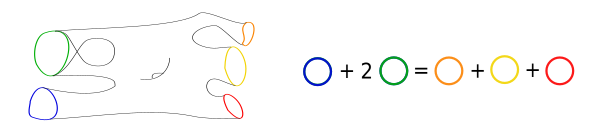
\includegraphics[width=1\textwidth]{reu_figures/motivational_homology.png}
    \label{fig:motivational_homology}
    \caption{This is a picture of two elements of $\op{ker}(\partial)$ as described above (the sum of the green and blue curves and the sum of the red, orange and yellow curves) along with the relation imposed by the fact that they mutually bound an surface.}
\end{figure}

We now move on to the actual, algebraic definition of homology and cohomology. The definition should make some sense with the above motivation in mind.

\begin{definition} \label{def:chain_complexes} (Chain Complexes) A {\bf chain complex} $(C,\partial)$ is a pair of an abelian group $C$, the {\bf chain group}, and a group homomorphism $\partial:C \to C$, the {\bf differential}. This pair must satisfy:
\begin{itemize}
\item[(a)] (Grading) The chain group $C$ decomposes as a direct sum $C = \oplus_{i \in \Z} C_i$.
\item[(b)] (Differential) The differential satisfies $\partial(C_i) \subset C_{i-1}$ and $\partial^2 = 0$.
\end{itemize}
A {\bf chain map} or morphism of chain complexes $f:(C,\partial) \to (D,\partial)$ is a map of abelian groups such that:
\begin{itemize}
\item[(a)] (Grading) $f$ respects the direct sum decomposition: $f(C_i) \subset D_i$.
\item[(b)] (Differential) $f$ commutes with the differential: $\partial f = f \partial$.
\end{itemize}
\end{definition}

\begin{definition} \label{def:homology} (Homology) The {\bf homology} $H(C,\partial)$ of a chain complex $(C,\partial)$ is the quotient abelian group defined as:
\[
H(C,\partial) := \op{ker}(\partial)/\op{image}(\partial)
\]
The homology also has a direct sum decomposition $H(C,\partial) = \oplus_{i \in \Z} H_i(C,\partial)$ with:
\[
H_i(C,\partial) := \op{ker}(\partial:C_i \to C_{i-1})/\op{image}(\partial:C_{i+1} \to C_i)
\]
Given an $a \in \op{ker}(\partial)$, we denote the image under the quotient $\op{ker}(\partial) \to H(C,\partial)$ as $[a]$. In this situation, we say that $a$ is a {\bf representative} of $[a]$ and we refer to $[a] \in H(C,\partial)$ as a {\bf cohomology class}. If $[a] \in H_i(C,\partial)$, we say that $[a]$ is {\bf degree} $i$ and use the notation $\op{deg}([a]) = i$. 

The {\bf induced map} $H(f):H(C,\partial) \to H(D,\partial)$ of a chain map $f:(C,\partial) \to (D,\partial)$ is defined, for any homology class $[a]$ and representative $a$, to be:
\[
H(f)[a] = [f(a)]
\]
\end{definition}

There is a dual notion called cohomology that arises naturally in several contexts (see \S \ref{subsec:de_rham_cohomology} for instance). The definition is very similar to Definition \ref{def:homology}, but we state it in full for maximum clarity.

\begin{definition} \label{def:cochain_complex} (Cochain Complexes) A {\bf cochain complex} $(C,d)$ is a pair of an abelian group $C$, the {\bf cochain group}, and a group homomorphism $d:C \to C$, the {\bf differential}. This pair must satisfy:
\begin{itemize}
\item[(a)] (Grading) The chain group $C$ decomposes as a direct sum $C = \oplus_{i \in \Z} C^i$.
\item[(b)] (Differential) The differential satisfies $\partial(C^i) \subset C^{i+1}$ and $d^2 = 0$.
\end{itemize}
A {\bf (co)chain map} or morphism of cochain complexes $f:(C,d) \to (D,d)$ is a map of abelian groups such that:
\begin{itemize}
\item[(a)] (Grading) $f$ respects the direct sum decomposition: $f(C^i) \subset D^i$.
\item[(b)] (Differential) $f$ commutes with the differential: $d f = f d$.
\end{itemize}
\end{definition}
\begin{definition} \label{def:cohomology} (Cohomology) The {\bf cohomology} $H(C,d)$ of $(C,d)$ is the quotient abelian group defined as:
\[
H(C,d) := \op{ker}(d)/\op{image}(d)
\] The cohomology also has a direct sum decomposition $H(C,d) = \oplus_{i \in \Z} H^i(C,d)$ with:
\[
H^i(C,d) := \op{ker}(d:C^i \to C^{i+1})/\op{image}(d:C^{i-1} \to C^i)
\]
Given an $a \in \op{ker}(d)$, we denote the image under the quotient $\op{ker}(d) \to H(C,d)$ as $[a]$. In this situation, we say that $a$ is a {\bf representative} of $[a]$ and we refer to $[a] \in H(C,d)$ as a {\bf cohomology class}. If $[a] \in H^i(C,d)$, we say that $[a]$ is {\bf degree} $i$ and use the notation $\op{deg}([a]) = i$. 

The {\bf induced map} $H(f):H(C,d) \to H(D,d)$ of a chain map $f:(C,d) \to (D,d)$ is defined, for any cohomology class $[a]$ and representative $a$, to be:
\[
H(f)[a] = [f(a)]
\]
\end{definition}

\begin{exercise} \label{ex:homology} Here are some exercises about homology. For these exercises, suppose that $(C,\partial)$ is a chain complex where $C_i$ is a vector-space over a field $\mathbb{F}$ and $\partial$ is $\mathbb{F}$-linear. 
\begin{itemize}
	\item[(a)] Give an example of a chain complex $(C,\partial)$ which is non-trivial but which has trivial homology, i.e. where $H(C,\partial) = \{0\}$ even though $C \neq \{0\}$. Give an example of a chain complex $(C,\partial)$ where $H(C,\partial) \simeq C$.
	\item[(b)] Define the {\bf dual cochain complex} $(\check{C}, \check{\partial})$ of $(C,\partial)$ as so:
	\[
	\check{C}^i := (C_i)^* \quad\text{and}\quad \check{\partial}:\check{C}^i \to \check{C}^{i+1} \text{ given by }\check{\partial}\alpha := \alpha \circ \partial = \partial^*\alpha
	\]
	\begin{enumerate}
		\item[(i)] Show that $\check{\partial}^2 = 0$, so that this truly defines a cochain complex.
		\item[(ii)] Show that a chain map $f:(C,\partial) \to (D,\partial)$ induces a cochain map $\check{f}:(\check{D},\check{\partial}) \to (\check{C},\check{\partial})$.
		\item[(iii)] Show that the dual pairing $C_i \times \check{C}^i \to \mathbb{F}$ descends to a well-defined pairing $H_i(C,\partial) \times H^i(\check{C},\check{\partial}) \to \mathbb{F}$. 

		To clarify, we have a map $C_i \times \check{C}^i \to \mathbb{F}$ given by $(a,\alpha) \mapsto \alpha(a)$. You need to show that if $[a] \in H_i(C,\partial)$ is represented by $a \in \op{ker}(\partial|_{C_i})$ and $[\alpha] \in H^i(\check{C},\check{\partial})$ is represented by $\alpha \in \op{ker}(\check{\partial}|_{\check{C}^i})$, then $\alpha(a)$ only depends on the classes $[\alpha]$ and $[a]$ (and not on the representatives) so that the map $H_i(C,\partial) \times H^i(\check{C},\check{\partial}) \to \mathbb{F}$ given by $([a],[\alpha]) \mapsto \alpha(a)$ is well-defined.
	\end{enumerate} 

	The same construction works if we replace $\mathbb{F}$ with a ring $R$. In that situation, we define the dual $(C_i)^*$ as $(C_i)^* := \op{Hom}_R(C_i,R)$, the module of $R$-linear maps from the module $C_i$ to $R$.
	\item[(c)] Suppose that $\op{dim}(C_i) < \infty$ for every $i$ and $\op{dim}(C_i) = 0$ for all but finitely many $i$. The {\bf Euler characteristic} $\chi(C,\partial)$ of $(C,\partial)$ is then defined to be:
	\[
	\chi(C,\partial) = \sum_i (-1)^i \op{dim}(C_i)
	\]
	Show that $\chi(C,\partial)$ is also given by the expression:
	\[
	\chi(C,\partial) = \sum_i (-1)^i \op{dim}(H_i(C,\partial))
	\]
	So it only depends on the homology of $(C,\partial)$.
\end{itemize}
\end{exercise}

\subsection{Singular Homology} \label{subsec:singular_homology} In this section, we define the most basic version of the homology of a manifold, namely singular homology $H^{\op{sg}}(X;R)$ with coefficients in a ring $R$. Singular homology can be viewed as a rigorous version of the non-rigorous construction in Motivation \ref{mot:groups_of_sub_manifolds}, where the $n$th chain group is generated by maps from a specific $n$-manifold-like object, namely the $n$-simplex $\Delta^n$, instead of maps from any $n$-dimensional manifold with boundary. 

In this sub-section, we define singular homology and discuss some of its important properties. We will also discuss the homological version of orientations.

\begin{notation} (Simplices) We adopt the following notation throughout this section. We denote by $\Delta^n$ the $n$-simplex, which we realize as the following subspace of $\R^{n+1}$:
\[
\Delta^n := \{x = (x_0,\dots,x_n) \in \R^{n+1}|x_i \ge 0 \text{ for all $i$ and }\sum_i x_i = 1\}
\]
For each $i \in \{0,\dots,n\}$ we denote by $\iota^n_i:\Delta^{n-1} \to \Delta^n$ the inclusion given by:
\[
\iota^n_i(x_0,\dots,x_{i-1},x_i,x_n) := (x_0,\dots,x_{i-1},0,x_i,\dots,x_n)
\]
\end{notation}

\noindent We will require the following Lemma. The proof is a direct computation.

\begin{lemma} \label{lem:simplex_inclusion} As maps $\Delta^{n-2} \to \Delta^n$, we have $\iota^n_i \circ \iota^{n-1}_j = \iota^n_j \circ \iota^n_{i-1}$.
\end{lemma}

We are \emph{already} prepared to state the definition of singular homology!

\begin{definition} \label{def:singular_homology} (Singular Homology) Let $R$ be a ring and let $X$ be a topological space. The {\bf singular homology} of $X$ with $R$ coefficients, $H^{\op{sg}}(X;R) = \oplus_{i=0}^\infty H^{\op{sg}}_i(X;R)$, is defined to be the homology of the {\bf singular chain complex} $(C^{\op{sg}}(X;R), \partial)$ with $R$ coefficients. The {\bf singular cohomology} of $X$ with $R$ coefficients, $H_{\op{sg}}(X;R) = \oplus_{i=0}^\infty H_{\op{sg}}^i(X;R)$, is defined to be the cohomology of the dual complex $(C_{\op{sg}}(X,R),d) = (\check{C}^{\op{sg}}(X;R),\check{\partial})$ of $(C^{\op{sg}}(X;R),\partial)$ (see Exercise \ref{ex:homology}).

The complex $(C^{\op{sg}}(X;R), \partial)$ of $X$ is defined as so. Let $\op{Map}(\Delta^n,X)$ denote the set of continuous maps from the $n$-simplex $\Delta^n$ to $X$. The chain group $C^{\op{sg}}(X;R) = \oplus_{n=0}^\infty C^{\op{sg}}_n(X;R)$ is defined as:
\[
C^{\op{sg}}_n(X;R) := R \cdot \op{Map}(\Delta^n,X)
\]
The group on the right denotes formal linear combinations of maps $\sigma^n:\Delta^n \to X$. That is, an element $x \in C^{\op{sg}}_n(X;R)$ is of the form:
\[
x = \sum_{j=1}^k c_j \cdot \sigma^n_j
\]
Here $\sigma^n_j:\Delta^n \to X$ is a continuous map and $c_j \in R$ for all $j \in \{1,\dots,k\}$. The differential $\partial:C^{\op{sg}}_n(X;R) \to C^{\op{sg}}_{n-1}(X;R)$ is defined on any $\sigma^n \in \op{Map}(\Delta^n;X)$ by:
\[
\partial(\sigma^n) := \sum_{i=0}^n (-1)^i \sigma^n \circ \iota^n_i 
\]
By linearity, this extends to a map $\partial:C^{\op{sg}}(X;R) \to C^{\op{sg}}(X;R)$. 
\end{definition} 

\begin{lemma} The map $\partial:C^{\op{sg}}(X;R) \to C^{\op{sg}}(X;R)$ satisfies:
\[\partial(C^{\op{sg}}_i(X;R)) \subset C^{\op{sg}}_{i-1}(X;R) \quad\text{and}\quad \partial^2 = 0\]
Thus Definition \ref{def:singular_homology} does actually define a chain complex. 
\end{lemma}

\begin{proof} The fact that $\partial(C^{\op{sg}}_i(X;R)) \subset C^{\op{sg}}_{i-1}(X;R)$ is immediate from the definition. To check $\partial^2 = 0$, we just need to check that $\partial^2(\sigma^n) = 0$ for any $\sigma^n \in \op{Map}(\Delta^n;R)$. To do this, let $I = \{0,\dots,n\} \times \{0,\dots,n-1\}$ and let $J = \{(i,j)|j < i\}$. Using the definition of $\partial$, we can compute the following:
\[\partial^2(\sigma^n) = \partial(\sum_{i=0}^n (-1)^i \sigma^n \circ \iota^n_i) = \sum_{j=0}^{n-1} \sum_{i=0}^{n} (-1)^{i+j} \sigma^n \circ \iota^n_i \circ \iota^{n-1}_j \]
\[
= \sum_{(i,j) \in J} (-1)^{i+j}(\sigma^n \circ \iota^n_i \circ \iota^{n-1}_j + (-1)\sigma^n \circ \iota^n_j \circ \iota^{n-1}_{i-1}) = 0
\]
Here we use Lemma \ref{lem:simplex_inclusion}, which implies that $\sigma^n \circ \iota^n_i \circ \iota^{n-1}_j = \sigma^n \circ \iota^n_j \circ \iota^{n-1}_{i-1}$ as maps. 
\end{proof}

Now that we have defined singular homology and cohomology groups, let us turn to a discussion some of the key properties that the groups themselves have. These properties are often all one needs to be a user of singular homology. 

\begin{proposition} \label{prop:singular_homology_properties} (Properties Of Singular Homology) Singular homology and singular cohomology have the following properties.
\begin{itemize}
	\item[(a)] (Maps) A continuous map $f:X \to Y$ induces a map of $R$-modules $f^{\op{sg}}_*:H^{\op{sg}}_i(X;R) \to H^{\op{sg}}_i(X;R)$ and a map $f^*_{\op{sg}}:H^i_{\op{sg}}(Y;R) \to H^i_{\op{sg}}(X;R)$.
	\item[(b)] (Composition) If $g:X \to Y$ and $f:Y \to Z$ are continuous maps, then $(f \circ g)^{\op{sg}}_* = f^{\op{sg}}_*g^{\op{sg}}_*$ and $(f \circ g)_{\op{sg}}^* = g_{\op{sg}}^*f_{\op{sg}}^*$.
	\item[(c)] (Homotopy Invariance) If $f:X \to Y$ and $g:X \to Y$ are homotopic, then the maps of homology and cohomology are equal: $f^{\op{sg}}_* = g^{\op{sg}}_*$ and $f_{\op{sg}}^* = g_{\op{sg}}^*$.
	\item[(d)] (Dual Pairing) There is a dual pairing between cohomology and homology:
	\[H^i(X;R) \times H_i(X;R) \to R \qquad ([\alpha], [a]) \mapsto \langle [\alpha],[a]\rangle := \alpha(a)\]
	This pairing yields an isomorphism $H^i(X;R) \simeq (H_i(X;R))^*$ when $R$ is a field.
	\item[(e)] (Products/Kunneth) Let $\mathbb{F}$ is a field. Then there is a natural isomorphism:
	\[
	H^{\op{sg}}_i(X \times Y;\mathbb{F}) \simeq \bigoplus_{j + k = i} H_j^{\op{sg}}(X;\mathbb{F}) \otimes H_j^{\op{sg}}(Y;\mathbb{F})
	\]
	\[
	H_{\op{sg}}^i(X \times Y;\mathbb{F}) \simeq \bigoplus_{j + k = i} H^j_{\op{sg}}(X;\mathbb{F}) \otimes H^j_{\op{sg}}(Y;\mathbb{F})
	\]
	These isomorphisms are compatible with the pushforward and pullback maps in the following sense: given manifolds $X_i,Y_i$ and maps $f_i:X_i \to Y_i$ for $i \in \{0,1\}$, we have:
	\[
	(f_0 \times f_1)_{\op{sg}}^* = (f_0)_{\op{sg}}^* \otimes (f_1)_{\op{sg}}^*
	\]
	\[
	(f_0 \times f_1)^{\op{sg}}_* = (f_0)^{\op{sg}}_* \otimes (f_1)^{\op{sg}}_*
	\]
	\end{itemize}
\end{proposition}

\begin{proof} (Partial) We will prove (a) and (b). We will provide pictures for (c) and (e) in Motivation, but the proofs are too involved to go in to in these notes. In particular, (c) requires a discussion of chain homotopies. (d) is a consequence of Exercise \ref{ex:homology}(a)(iii).

To prove (a) and (b), we construct a chain map associated to $f:X \to Y$:
\[C^{\op{sg}}(f):C^{\op{sg}}(X,\partial) \to C^{\op{sg}}(Y,\partial)\]
This chain map is defined as so: for any continuous map $\sigma:\Delta^n \to X$, i.e. a generator of $C^{\op{sg}}_n(X;R)$, we define $C^{\op{sg}}(f)$ by left composition:
\[C^{\op{sg}}(f)\sigma := f \circ \sigma\]
Then we extend the map to $C^{\op{sg}}_n(X;R)$ by linearity. $C^{\op{sg}}(f)$ clearly preserves the direct sum decomposition, and it commutes with $\partial$ since:
\[
C^{\op{sg}}(f)\partial\sigma = C^{\op{sg}}(f)(\sum_{i=0}^n (-1)^i \sigma \circ \iota^n_i) = \sum_{i=0}^n (-1)^i C^{\op{sg}}(f)(\sigma \circ \iota^n_i)
\]
\[
 = \sum_{i=0}^n (-1)^i f \circ \sigma \circ \iota^n_i = \sum_{i=0}^n (-1)^i (C^{\op{sg}}(f)\sigma) \circ \iota^n_i = \partial C^{\op{sg}}(f)\sigma
\]
We have thus shown that $C(f)$ is a chain map. We define $f^{\op{sg}}_*$ and $f_{\op{sg}}^*$ to be the induced map on homology and the induced map of the dual map on cohomology (see Exercise \ref{ex:homology}(a)(ii)). This proves (a), while (b) follows from the definition since:
\[
C^{\op{sg}}(f)C^{\op{sg}}(g)\sigma = f \circ g \circ \sigma = C^{\op{sg}}(f \circ g)\sigma
\]
Note that both properties ultimately come down to the fact that map composition is associative. \end{proof}

\begin{motivation} (Homotopy Invariance) We now provide an intuitive explanation for the property in Proposition \ref{prop:singular_homology_properties}(c) in terms of Motivation \ref{mot:groups_of_sub_manifolds}. 

Recall that in the intuitive picture of Motivation \ref{mot:groups_of_sub_manifolds}, a homology class $[\Sigma,\iota] \in H_n(X;\mathbb{F}_2)$ is an equivalence class of maps $\iota:\Sigma \to X$ from a closed manifold $X$, where any two representatives $(\Sigma_0,\iota_0)$ and $(\Sigma_1,\iota_1)$ must be related in the following way: there exists an $(n+1)$-manifold $Y$ and a map $j:Y \to X$ such that $\partial Y = \Sigma_0 \sqcup \Sigma_1$ and $j|_{\Sigma_i} = \iota_i$.

Now imaging that we had two maps $f_0,f_1:X \to Y$ homotopic via a map $f:X \times [0,1] \to Y$, $(x,t) \mapsto f_t(x)$. In Proposition \ref{prop:singular_homology_properties}, we defined the maps on homology induced by $f_i$ using left composition with $f_i$. In terms of Motivation \ref{mot:groups_of_sub_manifolds}, this means a representative $(\Sigma,\iota)$ of $[\Sigma,\iota] \in H_n(X;\mathbb{F}_2)$ is sent to $(\Sigma,f_i \circ \iota)$. Showing that these two representatives mutually bound something is simple: we simply take $Y = \Sigma \times [0,1]$ and define $j = f \circ \kappa$. Here $f:X \times [0,1] \to Y$ is the homotopy and $\kappa:\Sigma \times [0,1] \to X \times [0,1]$ is given by $\kappa(\sigma,t) = (\iota(\sigma),t)$. This clearly gives a bounding $(Y,j)$ for the pair $(\Sigma_0,f_0 \circ \iota)$ and $(\Sigma_1,f_1 \circ \iota)$, so that:
\[
(f_0)_*[\Sigma,\iota] = [\Sigma,f_0 \circ \iota] = [\Sigma,f_1f \circ \iota] = (f_1)_*[\Sigma,\iota]
\]
See Figure \ref{fig:chain_homotopy_picture} below for a drawing of the situation that we describe here.
\end{motivation}

\begin{figure}[h]
    \centering
    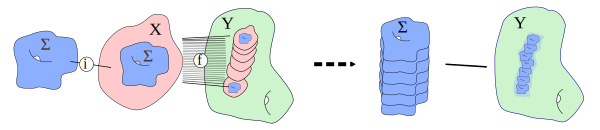
\includegraphics[width=1\textwidth]{reu_figures/homotopy_picture.png}
    \label{fig:chain_homotopy_picture}
    \caption{A depiction of how a homotopy of maps $f:X \times [0,1] \to Y$ from $X$ to $Y$ yields an object bounding $f_0(\iota(\Sigma))$ and $f_1(\iota(\Sigma))$, namely the cylinder over $\Sigma$ that is traced out by the homotopy.}
\end{figure}

We now move on to a discussion of (homological) orientations and their properties. An orientation of this form turns out to be the same data as the information of a section of the orientation bundle (see Proposition \ref{def:bundles_on_smooth_manifolds}(5)), although arguing this requires the introduction of relative homology and thus is beyond the scope of these notes.

\begin{definition} (Orientations) A closed $n$-manifold $X$ is {\bf orientable} if the $n$-th singular homology group satisfies $H^{\op{sg}}_n(X;\Z) \simeq \Z$. An {\bf orientation} of $X$ is a choice of generator $[X]$ of $H^{\op{sg}}_n(X;\Z)$ as an abelian group. The generator $[X]$ is also referred to as a {\bf fundamental class} of $X$.

An {\bf oriented} manifold is a pair $(X,[X])$ of a manifold $X$ and an fundamental class $[X]$ of $X$. In general, we suppress the orientation in the notation for an oriented manifold. A smooth map $f:X \to Y$ is {\bf orientation preserving} if $f_*[X] = [Y]$.
\end{definition}

\begin{motivation} (Fundamental Classes) Using the intuition of Motivation \ref{mot:groups_of_sub_manifolds}, we want to think of a fundamental class $[X]$ of $X$ as a closed sub-manifold of $X$ that is the same dimension as $X$ itself. In fact, we should think of the class $[X]$ as representing $X$ itself. 

The fundamental class also makes one of the key intuitions from Motivation \ref{mot:groups_of_sub_manifolds} rigorous. Namely, we want to think of a homology class $[a]$ as being represented by a map $\iota:\Sigma \to X$ of $k$-dimensional closed manifold $\Sigma$ into $X$. We can use the fundamental class to (almost) realize this idea via the following result of Thom.
\end{motivation}

\begin{proposition} (c.f. \cite{sullivan2004}) Let $X$ be a manifold and let $[a] \in H_k^{\op{sg}}(X;\Z)$ be an integral homology class. Then there exists an oriented closed $k$-manifold $\Sigma$, a map $\iota:\Sigma \to X$ and a $k \in \Z^+$ such that $\iota^{\op{sg}}_*[\Sigma] = k[a]$.
\end{proposition}

\subsection{Simplicial Homology} \label{subsec:simplicial_homology} While singular homology groups are very easy to define, it is quite difficult to compute them using only Definition \ref{def:singular_homology}. A remedy for this is to define different homology groups that are easier to calculate directly from the definition, but which end up being isomorphic in the end. This computational utility comes at a price, however. It is much more difficult to directly demonstrate the many nice properties that singular homology possesses (see Proposition \ref{prop:singular_homology_properties}) directly for simplicial homology. 

In this sub-section, we will explain how to define the simplicial homology of a very combinatorial object called a simplicial complex\footnote{We will use our own definition of simplicial complex. There are many definitions that are equivalent for the most part}. In \S \ref{subsec:relationships_of_homologies}, we will explain how to turn a simplicial complex into a topological space, and how the simplicial homology of the set is related to the singular homology of the space.

\begin{definition} \label{def:simplicial_complex} (Simplicial Complex) A {\bf simplicial complex} $\mathcal{S} = (F,\preccurlyeq,\op{dim},\sigma)$ consists of the following data\footnote{This is a slightly non-standard definition of an abstract simplicial complex. We use this definition to emphasize the precise combinatorial data needed to compute simplicial homology.}:
\begin{enumerate}
	\item[(a)] A finite, partially ordered set $(F,\preccurlyeq)$ called the {\bf facet set}.
	\item[(b)] An order preserving function $\op{dim}:F \to \Z^+ \cup \{0\}$ called the {\bf dimension}.
	\item[(c)] An injective map $\sigma^f_e:\{0,\dots,\op{dim}(e)\} \to \{0,\dots,\op{dim}(f)\}$ for each $e,f \in P$ with $e \preccurlyeq f$, called the {\bf gluing map} from $e$ to $f$.
\end{enumerate}
The poset and gluing maps must satisfy the following properties:
\begin{enumerate}
\item[-] (Facet Closure And Uniqueness) For every $f \in F$ and $S \subset \{0,\dots,\op{dim}(f)\}$, there exists a unique $e \in F$ such that $e \preccurlyeq f$ and $\op{image}(\sigma^f_e) = S$.
\item[-] (Consistency) $\sigma^e_e = \op{Id}$ and $\sigma^g_e = \sigma^g_f \circ \sigma^f_e$ for any $e,f,g \in F$ with $e \preccurlyeq f \preccurlyeq g$.
\end{enumerate} 
\end{definition}

\begin{definition} \label{def:simplicial_homology} (Simplicial Homology) Let $R$ be a ring and let $\mathcal{S}$ be a simplicial complex. The {\bf simplicial homology} of $\mathcal{S}$ with $R$ coefficients, $H^{\op{sp}}(\mathcal{S};R) = \oplus_{i=0}^\infty H^{\op{sp}}_i(\mathcal{S};R)$, is defined to be the homology of the {\bf simplicial chain complex} $(C^{\op{sp}}(\mathcal{S};R), \partial)$ with $R$ coefficients. The {\bf singular cohomology} of $\mathcal{S}$ with $R$ coefficients, $H_{\op{sp}}(\mathcal{S};R) = \oplus_{i=0}^\infty H_{\op{sp}}^i(\mathcal{S};R)$, is defined to be the cohomology of the dual complex $(C_{\op{sp}}(\mathcal{S};R),d) = (\check{C}^{\op{sp}}(\mathcal{S};R),\check{\partial})$ of $(C^{\op{sp}}(\mathcal{S};R),\partial)$ (see Exercise \ref{ex:homology}).

The complex $(C^{\op{sp}}(\mathcal{S};R),\partial)$ is defined a so. Set $C^{\op{sp}}(\mathcal{S};R) = \oplus_n C_n^{\op{sp}}(\mathcal{S};R)$ to be:
\[
C_n^{\op{sp}}(\mathcal{S};R) := R \cdot \{f \in F|\op{dim}(f) = n\}
\]
The group on the right denotes formal linear combination of faces $f \in F$ with $\op{dim}(f) = n$ with $R$ coefficients. The differential $\partial:C^{\op{sp}}_n(\mathcal{S};R) \to C^{\op{sp}}_{n-1}(\mathcal{S};R)$ is defined on any $f$ with $\op{dim}(f) = n$ as:
\[
\partial(f) = \sum_{\substack{\op{dim}(e) + 1 = \op{dim}(f)\\ e \preccurlyeq f}} \op{sign}(\sigma^f_e) \cdot e
\]
Here the sign of a map $\sigma:\{0,\dots,d\}\to \{0,\dots,d+1\}$ is defined to be the sign (as a permutation) of the unique permutation $\bar{\sigma}:\{0,\dots,d+1\} \to \{0,\dots,d+1\}$ with the property that $\bar{\sigma}(i) = \sigma(i-1)$ for all $i > 0$.
\end{definition}

\begin{lemma} \label{lem:simplicial_d2_zero} The map $\partial:C^{\op{sp}}(\mathcal{S};R) \to C^{\op{sp}}(\mathcal{S};R)$ satisfies:
\[
\partial(C^{\op{sp}}_i(\mathcal{S};R)) \subset C^{\op{sp}}_{i-1}(\mathcal{S};R) \quad \text{and} \quad \partial^2 = 0
\]
Thus Definition \ref{def:simplicial_homology} does actually define a chain complex. 
\end{lemma}

\begin{proof} As with Definition \ref{def:singular_homology}, the fact that $\partial(C^{\op{sp}}_i(\mathcal{S};R)) \subset C^{\op{sp}}_{i-1}(\mathcal{S};R)$ is immediate. To show that $\partial^2 = 0$, we can show that $\partial^2(f) = 0$ for any $f \in F$. We compute that:
\[
\partial^2(f) = \partial\big(\sum_{\substack{\op{dim}(e) + 1 = \op{dim}(f)\\ e \preccurlyeq f}} \op{sign}(\sigma^f_e) \cdot e\big)
= \sum_{\substack{\op{dim}(d) + 2 = \op{dim}(f)\\ d \prec e \prec f}} \op{sign}(\sigma^e_d) \cdot \op{sign}(\sigma^f_e) \cdot d 
\]
In the latter sum, $d$ appears once for every chain $d \prec e \prec f$ where $\op{dim}(d) + 2 = \op{dim}(e) + 1 = \op{dim}(f)$. Due to the closure and uniqueness property of the facet set $F$ of $\mathcal{S}$ in Definition \ref{def:simplicial_complex}, such chains are in bijection with chains of subsets:
\[
\op{image}(\sigma^f_d) \subset S \subset \{0,\dots,\op{dim}(f)\}
\]
where $|S| = \op{dim}(e) + 1 = \op{dim}(f)$ and (of course) $|\op{image}(\sigma^f_d)| = \op{dim}(d) + 1 = \op{dim}(f) - 1$. There are clearly two such subets, and by Lemma \ref{lem:simplex_inclusion_a} the corresponding coefficients of these two $d$ terms cancel.
\end{proof}

\begin{lemma} \label{lem:simplex_inclusion_a} Consider injections of the form:
\[\sigma_d^e,\sigma_d^f:\{0,\dots,n\} \to \{0,\dots,n+1\}\]
\[\sigma_e^g,\sigma_f^g:\{0,\dots,n+1\} \to \{0,\dots,n+2\}\] 
Suppose that $\sigma^g_e\circ \sigma^e_d = \sigma^g_f \circ \sigma^f_d$ and $\op{image}(\sigma^g_e) \neq \op{image}(\sigma^g_f)$. Then:
\[
\op{sign}(\sigma^g_e) \cdot \op{sign}(\sigma^e_d) = - \op{sign}(\sigma^g_f) \cdot \op{sign}(\sigma^f_d)
\]
\end{lemma}

\begin{proof} Recall that the sign map $\op{sign}:\Sigma_{n+1} \to \{\pm 1\}$ from permutations of $\{0,\dots,n\}$ to $\{\pm 1\}$ is a group homomorphism. Using this, we can deduce that if $\rho:\{0,\dots,n\} \to \{0,\dots,n\}$ and $\tau:\{0,\dots,n+1\} \to \{0,\dots,n+1\}$ are permutations and $\sigma:\{0,\dots,n+1\} \to \{0,\dots,n+2\}$ is an injection, we have the multiplication property:
\[
\op{sign}(\tau \circ \sigma \circ \rho) = \op{sign}(\tau) \cdot \op{sign}(\sigma) \cdot \op{sign}(\rho)
\]
Here the signs of $\tau$ and $\rho$ are as permutations and the sign of $\sigma$ is by our definition. Now if we let $\tau_e,\tau_f$ and $\tau_g$ be permutations such that:
\[\tau_e \circ \sigma^e_d(i) = i+1 \qquad \tau_f \circ \sigma^f_d(i) = i+1 \qquad \tau_g \circ \sigma^g_e \circ \tau_e^{-1}(i) = i+1\] 
Then by the multiplication property, it suffices to verify our result where we make the replacements:
\[\sigma^e_d \implies \tau_e \circ \sigma^e_d \qquad \sigma^f_d \implies \tau_f \circ \sigma^f_d\]
\[\sigma^g_e \implies \tau_g \circ \sigma^g_e \circ \tau_e^{-1} \qquad \sigma^g_f \implies \tau_g \circ \sigma^g_f \circ \tau_f^{-1}\]
It is simple to check that under our assumptions, this reduces us to the case where:
\[
\sigma^e_d(i) = \sigma^f_d(i) = i+1 \qquad \sigma^g_e(i) = i+1 \qquad
\sigma^g_f(i) = 
\left\{\begin{array}{cc}
0 & \text{ if }i = 0\\
i+1 & \text{ otherwise }\\
\end{array}\right.
\]
Computing signs using the definition stated in \ref{def:simplicial_homology} yields:
\[
\op{sign}(\sigma^e_d) = \op{sign}(\sigma^f_d) = \op{sign}(\sigma^g_e) = 1 \qquad \op{sign}(\sigma^g_f) = -1
\]
This verifies the desired result in this case and concludes the proof.\end{proof}

Although the definitions are very different, there is a relationship between simplicial and singular homology. It turns out that, in the regimes where these theories overlap, they produce isomorphic groups. At this point, it is probably quite difficult to understand what we mean by this: singular homology groups are associated to spaces while simplicial homology groups are associated to simplicial complexes. Thus we must first explain how to take a simplicial complex and turn it into a space.

\begin{definition}
The {\bf geometric realization} $X_{\mathcal{S}}$ of a simplicial complex $\mathcal{S}$ is the space constructed as so. For each $f \in F$, we associate a copy $\Delta^f$ of the $\op{dim}(f)$-dimensional simplex $\Delta^{\op{dim}(f)}$. Given any $e \preccurlyeq f$, the gluing map $\sigma_e^f$ induces a map $\Delta^e \to \Delta^f$ given by:
\[
(x_0,\dots,x_{\op{dim}(e)}) \mapsto (y_0,\dots,y_{\op{dim}(f)}) \qquad 
y_i = 
\left\{\begin{array}{cc}
x_j & i = \sigma^f_e(j)\\
0 & \text{else} 
\end{array}\right.
\]
By abuse of notation, we denote this map by $\sigma^f_e:\Delta^e \to \Delta^f$. Finally, define $X_{\mathcal{S}}$ by:
\[
X_{\mathcal{S}} := \big(\bigsqcup_{f \in F} \Delta^f\big)/\sim
\]
Here $\sim$ is the equivalence relation defined to be the transitive closure of the relation $x \sim y$ if and only if $\sigma_e^g(x) = \sigma^g_f(y)$ for $e,f,g \in F$ with $e \preccurlyeq g$ and $f \preccurlyeq g$. Note that each facet $f \in F$ is associated to a continuous map $\sigma_f:\Delta^{\op{dim}(f)} \to X_{\mathcal{S}}$ given by:
\[
\sigma_f:\Delta^{\op{dim}(f)} \simeq \Delta^f \hookrightarrow \sqcup_{f \in F} \Delta^f \to X_{\mathcal{S}}
\]
Here the last map is the obvious quotient map.
\end{definition}

We can now state a result relating the simplicial homology of $\mathcal{S}$ and the singular homology of $X_{\mathcal{S}}$. We will not include a proof of this result, although a part of the proof will be given as an exercise.

\begin{proposition} (Simplicial Of $\mathcal{S}$ $\simeq$ Singular Of $X_{\mathcal{S}}$) Let $\mathcal{S} = (F,\preccurlyeq,\op{dim},\sigma)$ be a simplicial complex with geometric realization $X_{\mathcal{S}}$. Then the map $C^{\op{sp}}(\mathcal{S};R) \to C^{\op{sg}}(X_{\mathcal{S}};R)$ defined on a generator $f \in F$ of $C^{\op{sp}}(\mathcal{S};R)$ to be:
\[
f \in F \mapsto (\sigma_f:\Delta^{\op{dim}(f)} \to X_{\mathcal{S}}) \in \op{Map}(\Delta^{\op{dim}(f)}, X_{\mathcal{S}})
\]
is a chain map (see Definition \ref{def:chain_complexes}). Furthermore, the induced map yields a canonical isomorphism:
\[
\mathcal{SP}_{\mathcal{S}}:H^{\op{sp}}(\mathcal{S};R) \simeq H^{\op{sg}}(X_{\mathcal{S}};R)
\]
\end{proposition}

Of course, this result isn't that interesting to us unless we can expect to apply it to manifolds on a regular basis. The question of whether or not every manifold can be made using a simplicial complex has many variants, some of which were open until very recently. The following result is most relevant to us and is quite old. 

\begin{theorem} (c.f. \cite{cairns1935},\cite{whitehead1940}) Let $X$ be a compact smooth manifold with boundary has a simplicial complex $\mathcal{S}$ such that $X_{\mathcal{S}}$ and $X$ are homeomorphic.
\end{theorem}

These two results together allow us to utilize simplicial homology to compute singular homology. We will compute some examples this way later in this section, and in some exercises.

\begin{exercise} We will now compute the simplicial homology of several spaces.
\begin{itemize}
	\item[(a)] Compute the simplicial homology of the circle using the following simplicial complex $\mathcal{S}$ with $X_{\mathcal{S}} \simeq S^1$, depicted in Figure \ref{fig:simplicial_circle} below. Here the left-hand side gives the facet set, the dimensions of each facet, and the gluing maps in the form of a labeled graph. The right-hand side shows the geometric realization.
	\item[(b)] Compute the simplicial homology of the $2$-sphere using the simplicial structure of the boundary of a $3$-simplex. Feel free to ask for more details.
	\item[(c)] Determine a simplicial complex $\mathcal{S}$ whose geometric realization is $\R P^2$ and use it to compute the homology if $\R P^2$. (Hint: $\R P^2$ is the quotient of the upper-hemisphere of $S^2$ in $\R^3$ by some identification of oposite points on the boundary of the hemisphere. Give a similar description in terms of a square based pyramid.)
\end{itemize}
\end{exercise}

	\begin{figure}[h]
    \centering
    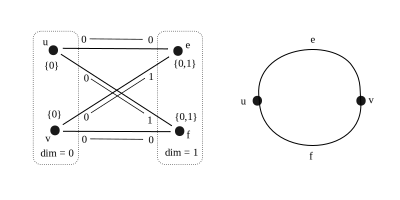
\includegraphics[width=1\textwidth]{reu_figures/circle_simplicial.png}
    \label{fig:simplicial_circle}
    \caption{A simplicial complex for the circle.}
		\end{figure}

\subsection{De Rham Cohomology} \label{subsec:de_rham_cohomology} In this section, we define de Rham cohomology. We have already seen all of the ingredients for this theory, so the definition is extremely fast! On the other hand, he proof that this theory is related to the others from \S \ref{subsec:singular_homology} and \S \ref{subsec:simplicial_homology} is too difficult for us to discuss here, although we will give an overview of this fact in Theorem \ref{thm:de_rham_and_sing}.

\begin{definition} \label{def:de_rham_cohomology} (De Rham Cohomology) Let $X$ be a closed manifold. The {\bf de Rham cochain complex} is the cochain complex $(\Omega(X),d)$. Here the cochain group is the vector-space $\Omega(X) = \oplus_{i=0}^n \Omega^i(X)$ of differential forms and the differential $d:\Omega(X) \to \Omega(X)$ is the exterior derivative (see Definition \ref{def:exterior_derivative}). The {\bf de Rham cohomology} $H^i_{dR}(X)$ is the cohomology:
\[
H^i_{dR}(X) := H^i(\Omega(X),d)
\]
\end{definition}

As we did in Proposition \ref{prop:singular_homology_properties}, we now turn to a discussion some of the key properties of de Rham cohomology. These properties are very similar to those in Proposition \ref{prop:singular_homology_properties}, and this is no accident: as we will see later. 

\begin{proposition} \label{prop:de_rham_homology_properties} (Properties Of De Rham Cohomology) De Rham cohomology has the following properties.
\begin{itemize}
	\item[(a)] (Maps) A smooth map $f:X \to Y$ induces a linear map $f^*_{\op{dR}}:H^i_{\op{dR}}(Y) \to H^i_{\op{dR}}(X)$ given in terms of the pullback $f^*:\Omega(Y) \to \Omega(X)$ by:
	\[f^*_{\op{dR}}[\omega] = [f^*\omega]\]
	\item[(b)] (Composition) If $g:X \to Y$ and $f:Y \to Z$ are smooth maps then:
	\[(f \circ g)_{\op{dR}}^* = g_{\op{dR}}^*f_{\op{dR}}^*\]
	\item[(c)] (Homotopy Invariance) If $f:X \to Y$ and $g:X \to Y$ are smoothly isotopic, then the maps of de Rham cohomology are equal: $f_{\op{dR}}^* = g_{\op{dR}}^*$.
	\item[(d)] (Dual Pairing) Given any oriented closed $k$-manifold $\Sigma$ and smooth map $\iota:\Sigma \to X$, the linear map $H^i_{\op{dR}}(X) \to \R$ given by:
	\[[\omega] \mapsto \int_{\Sigma} \iota^*\omega\]
	is well-defined (indpendent of the representative $\omega$ of $[\omega]$) and thus defines an element $[\Sigma,\iota] \in (H^i_{\op{dR}}(X))^*$.
	\item[(e)] (Products/Kunneth) Let $\mathbb{F}$ is a field. Then there is a natural isomorphism:
	\[
	H_{\op{dR}}^i(X \times Y) \simeq \bigoplus_{j + k = i} H^j_{\op{dR}}(X) \otimes H^j_{\op{dR}}(Y)
	\]
	For a pure tensor $[\alpha] \otimes [\beta] \in H^j_{\op{dR}}(X) \otimes H^j_{\op{dR}}(Y)$, this isomorphism can be written explicitly as:
	\[
	[\alpha] \otimes [\beta] \mapsto [\pi^*_X\alpha \wedge \pi^*_Y\beta]
	\]
	Given closed manifolds $X_i,Y_i$ and maps $f_i:X_i \to Y_i$ for $i \in \{0,1\}$, we have:
	\[
	(f_0 \times f_1)_{\op{dR}}^* = (f_0)_{\op{dR}}^* \otimes (f_1)_{\op{dR}}^*
	\]
	\end{itemize}
\end{proposition}

\begin{proof} (Partial) We will prove most of this proposition. However, we skip the proof of (e) since it is (again) a bit too technical to go in to. It is nice to see, however, that the formula for (e) is so explicit in this case.

We have already done the work for (a). Namely, we proved that $f^*(d\omega) = d(f^*\omega)$ and that $f^*:\Omega^i(Y) \to \Omega^i(X)$, so that it preserves the grading. Thus $f^*$ is a (co)chain map and induces a map $f^*_{\op{dR}}:H^i_{\op{dR}}(Y) \to H^i_{\op{dR}}(X)$. The composition property (b) follows from the fact that $g^*f^*\omega = (f \circ g)^*\omega$. 

Now we prove (c). Unlike in Proposition \ref{prop:singular_homology_properties}, we have the tools to do it. Let $h:X \times [0,1] \to Y$ be an isotopy between $f = h_0$ and $g = h_1$ and let $\omega$ be a closed $k$-form on $Y$. We need to show that $f^*\omega - g^*\omega = d\alpha$ for some $\alpha \in \Omega^{k-1}(Y)$. By the isotopy extension theorem, we can find an ambient isotopy $j:Y \times [0,1] \to Y$ such that $h_t = j_t \circ h_0 = j_t \circ f$ for any $t \in [0,1]$ and $j_0 = \op{Id}$. By the composition property (b), we know that $f^*\omega = j_0^*f^*\omega$ and $g^*\omega = j_1^*f^*\omega$. Redefining $\omega$ to be $f^*\omega$, and $h$ itself to be $j$, we can thus reduce to the case where $X = Y$ and $h:X \to X$ is an ambient isotopy.

Under this simplifying assumption, we proceed as so. Let $Z$ be the time-dependent vector-field defined implicitly by the equation:
\[
\frac{dh_t}{dt}|_{t = s} = Z_s \circ h_s
\]
We can compute the following identity for the time-derivative of $h^*_t\omega$ in terms of $Z_s$.
\[
\frac{d}{dt}(h_t^*\omega)|_{t = s} = \mathcal{L}_{Z_s}h^*_s\omega = \iota_{Z_s}d(h^*_s\omega) + d(\iota_{Z_s}\omega)  = d(\iota^*_{Z_s}\omega)
\]
Here we use the fundamental identity of the Lie derivative, Cartan's magic formula and the closedness of $\omega$. We can then integrate to see that:
\[
g^*\omega - f^*\omega = h_1^*\omega - h^*_0\omega = \int_0^1 d(\iota_{Z_s}\omega) dt = d(\int_0^1 \iota_{Z_s}\omega dt) = d\sigma
\]
This concludes the proof of (c).

The dual pairing property (d) follows from Stoke's theorem. In particular, if $[\omega]$ is represented by $\omega$ and $\omega'$, then:
\[
\int_\Sigma \iota^*\omega - \iota^*\omega' = \int_\Sigma \iota^*(\omega - \omega') = \int_\Sigma d(\iota^*\sigma) = \int_{\partial \Sigma} \iota^*\sigma = 0
\]
This concludes the parts of the proof that we set out to do. \end{proof}

We now turn to the relationship between de-Rham and singular cohomology. We don't have to do any preparatory work here to state the relevant result. There is already a regime in which both theories are well-defined, namely on closed manifolds. 

\begin{theorem} \label{thm:de_rham_and_sing} (De Rham) Let $X$ be a closed manifold. Then there is a natural isomorphism:
\[
\mathcal{DR}_X:H^i_{dR}(X) \simeq H^i_{\op{sing}}(X;\R)
\]
This isomorphism has the following properties.
\begin{itemize}
\item[(a)] (Pullback) $\mathcal{DR}$ is compatible with pullback in the sense that if $f:X \to Y$ is a smooth map of closed manifolds, then:
\[
f_{\op{sg}}^* \circ \mathcal{DR}_Y = \mathcal{DR}_X \circ f^*_{\op{dR}}
\]
\item[(b)] (Dual Pairing) $\mathcal{DR}$ is the following sense. If $\Sigma$ is a closed, oriented manifold and $\iota:\Sigma \to X$ is smooth, then:
\[
\langle \mathcal{DR}_X([\omega]),\iota^*_{\op{sg}}[\Sigma]\rangle = \langle \iota^*_{\op{dR}}[\omega],[\Sigma,\iota]\rangle = \int_\Sigma \iota^*\omega
\]
\item[(b)] (Product) $\mathcal{DR}$ is compatible with the Kunneth isomorphism in the sense that if $X$ and $Y$ are closed manifolds, then: 
\[
\mathcal{DR}_X([\alpha]) \times \mathcal{DR}_Y([\beta]) = \mathcal{DR}_{X \times Y}(\pi_X^*[\alpha] \wedge \pi_Y^*[\beta]) \in H^i_{\op{sing}}(X \times Y;\R)
\]
\end{itemize}
\end{theorem}

\begin{exercise} Here are some exercises about de Rham cohomology. 
\begin{itemize}
	\item[(a)] Show that the wedge product $\wedge:\Omega(X) \otimes \Omega(X) \to \Omega(X)$ descends to a product on the de Rham cohomology. That is the product:
	\[
	[\alpha] \otimes [\beta] \mapsto [\alpha \wedge \beta]
	\]
	gives a well-defined bilinear product on $H_{\op{dR}}(X)$.
\end{itemize}
\end{exercise} 

\section{Symplectic And Contact Geometry} \label{sec:symplectic_and_contact_manifolds} In this section, we finally get to the objective of these notes: a discussion of elementary symplectic and contact geometry. 

\subsection{Translating Hamiltonian Mechanics} \label{subsec:translating_mechanics} The first step will be to translate the theory of Hamiltonian mechanics as described in \S \ref{subsec:newton_to_hamilton}-\ref{subsec:hamilton_to_symplectic} into manifold theoretic language. Thus we return, after our long wayward journey, so the realm of \S \ref{sec:introduction}. This translation can be summarized in the following table, which we elaborate on below.

\begin{center}
\begin{tabular}{|c|c|}
\hline
Hamiltonian Mechanics & Symplectic Geometry\\
\hline 
\hline
phase space $\R^{2n} = \R^n_x \times \R^n_p$ & symplectic manifold $X$\\
\hline
bilinear form $\omega_0 = \langle J \cdot,\cdot\rangle$ & symplectic form $\omega \in \Omega^2(X)$\\
\hline
Hamiltonian $H \in C^\infty(\R^{2n})$ & Hamiltonian $H \in \Omega^0(X)$\\
\hline
gradient $\nabla H \in C^\infty(\R^{2n},\R^{2n})$ & exterior derivative $dH \in \Omega^1(X)$\\
\hline
vector-field $-J\nabla H \in C^\infty(\R^{2n},\R^{2n})$ & Hamiltonian vector-field $X_H$ s.t. $\iota_{X_H}\omega = dH$\\
\hline
Hamilton's equation $\frac{d\gamma}{dt} = -J\nabla H \circ \gamma$ & Hamilton's equation $\frac{d\gamma}{dt} = X_H \circ \gamma$\\
\hline
time evolution $\R \times \R^{2n} \to \R^{2n}$ & Hamiltonian flow $\Phi_H:\R \times X \to X$\\
\hline
\end{tabular}
\end{center}

We now discuss the parts of this table. First, we look for a replacement for the phase spaces $\R^n_x \times \R^n_p$ in manifold land: the clear candidates are just manifolds of dimension $2n$. Similarly, the trajectories of particles $\gamma:\R \to \R^n_x \times \R^n_p$ should be relaced with maps $\gamma:\R \to X$ and the flow $\Phi^H:\R^n_x \times \R^n_p \times \R_t \to \R^n_x \times \R^n_p$ given by ``flowing by time $t$'' should be replaced with an ambient isotopy $\Phi^H:X \times \R \to X$. The gradient of a Hamiltonian energy function $H:X \to \R$ should be replaced with the differential $dH:TX \to X \times \R$ (since this is the coordinate invariant version of the gradient, or at-least its dual) and the Hamiltonian vector-field $X^H$ that satisfied $X_H = -J\nabla H$ should be replaced by a vector-field $X^H$. 

Now we look for a replacement for the bilinear form $\langle J \cdot,\cdot\rangle$. Recall the roll that this played in Hamiltonian mechanics in regular phase space. Namely, we could define the Hamiltonian vector-field $X_H$ implicitly via the equation:
\[
\langle \nabla H,v\rangle = \langle JX_H,v\rangle \quad \text{for any $v \in \R^n_x \times \R^n_p$}
\]
Our goal is to find a replacement $\omega$ for $\omega_0$ that shares any properties of $\omega_0$ that are coordinate independent (meaning that we can be stated in the context of a manifold, without reference to any particular chart).

If we let $X = \R^n_x \times \R^n_p$ write this as an equation on the tangent space $TX$ at a point $x \in X$ and using $v \in T_xX$, $dH, X^H$ and $\omega_0$, this says that:
\[
dH_x(v) = \omega_0(X^H_x,v)
\]
In other words, the replacement $\omega$ for $\omega_0$ on $X$ needs to be a bilinear pairing $TX \otimes TX \to X \times \R$ at each point. Furthermore, the pairing must have the following two properties that $\omega_0$ has, both of which can be stated independent of chart.
\begin{itemize}
	\item[(a)] $\omega$ must be \emph{non-degenerate} as a pairing on each fiber $T_xX \otimes T_xX \to \R$, meaning that for any $x \in X$ and non-zero $u \in T_xX$ there exists a $v \in T_xX$ such that $\omega_x(u,v) \neq 0$. This certainly holds for $\omega_0$, since if $u = -Jv$ then:
	\[
	\omega_0(u,v) = \langle Ju,v\rangle = \langle -J^2 v,v\rangle = \langle v,v\rangle > 0
	\]
	\item[(b)] $\omega$ must be \emph{anti-symmetric}, meaning $\omega_x(u,v) = -\omega_x(v,u)$. This is also a property that $\omega_0$ has:
	\[
	\omega_0(u,v) = \langle Ju,v\rangle = v^TJu =(v^TJu)^T = u^TJ^Tv = -u^TJv = -\omega_0(v,u)
	\]
\end{itemize}

The final property that $\omega$ must have is tied to the way that it is preserved by the Hamiltonian flow. One can easily check that $\omega_0$ is preserved by the flow in the sense that:
\[
\omega_0(d\Phi_t(u),d\Phi_t(v)) = \omega_0(u,v) \text{ for any }u,v \in \R^n_x \times \R^n_p
\]

\subsection{Symplectic Manifolds} \label{subsec:symplectic_and_contact_manifolds} In this section, we formalize the discussion above in \S \ref{subsec:translating_mechanics}. We define symplectic manifolds, Hamiltonians and their vector-fields, 

\begin{definition} (Symplectic Manifolds) A {\bf symplectic $2n$-manifold} $(X,\omega)$ is a pair of a $2n$-manifold $X$ and $2$-form $\omega \in \Omega^2(X)$ such that:
\begin{enumerate}
	\item[(a)] $\omega$ is closed, i.e. $d\omega = 0$.
	\item[(b)] The $2n$-form $\omega^n$ is a volume form, i.e. $\omega^n \neq 0$ fiber-wise.
\end{enumerate}
The $2$-form $\omega$ is called the {\bf symplectic form} or {\bf symplectic structure}.
\end{definition}

For the remainder of this section, let $(X,\omega)$ be a symplectic manifold.

\begin{definition} (Hamiltonians)  A {\bf Hamiltonian} $H$ on $X$ is a smooth function $H:X \to \R$. A {\bf time-dependent} Hamiltonian is a function $H:X \times U \to \R$ where $U \subset \R$ is some (open or closed) interval of $\R$. A time-dependent Hamiltonian $H:X \times \R \to \R$ is {\bf $T$-periodic} if $H_{t + T}(x) = H_t(X)$ for all $(x,t) \in X \times \R$. In that case we can interpret $H$ as a map $H:X \times \R/T\Z \to \R$.

The {\bf Hamiltonian vector-field} $X^H$ of a Hamiltonian $H:X \times U \to \R$ is the unique time-dependent vector-field (i.e. section of $\pi_X^*TX$ over $X \times U$) that satisfies $\iota(X^H_t)\omega = dH_t$ for each $t$. Any time-dependent Hamiltonian $H:X \times \R \to \R$ generates a family of diffeomorphisms $\Phi^H:X \times \R \to \R$ given by:
\[
\frac{d\Phi^H}{dt}|_{t = s} = X_{H_s} \circ \Phi^H_s \quad\text{and}\quad \Phi^H_0  = \op{Id}
\]
When $H$ is time-independent, this is called the {\bf Hamiltonian flow} of $H$.
\end{definition}

\begin{definition} (Maps Of Symplectic Manifolds) Let $(X_0,\omega_0)$ and $(X_1,\omega_1)$ be symplectic manifolds.
\begin{enumerate}
	\item[(a)] A {\bf symplectic diffeomorphism} or {\bf symplectomorphism} $\varphi:X_0 \to X_1$ is a diffeomorphism satisfying $\varphi^*\omega_1 = \omega_0$
	\item[(b)] A {\bf Hamiltonian diffeomorphism} $\varphi:X_0 \to X_1$ is a symplectomorphism such that there exists a Hamiltonian $H:X \times [0,1] \to \R$ with $\varphi = \Phi^H_1$.
\end{enumerate}
\end{definition}

\begin{example} Here are some examples of symplectic manifolds.
\begin{enumerate}
	\item[(a)] (Phase Space) Euclidean space $\R^{2n} = \R^n_x \times \R^n_p$, with coordinates $x_i,p_i$ for $i \in \{1,\dots,n\}$, is symplectic with symplectic form $\omega_0 = \sum_{i=1}^n dx_i \wedge dp_i$
	\item[(b)] (Surfaces) Let $\Sigma$ be an orientable surface. Then $\Lambda^2\Sigma$ is trivial, so we can pick a non-vanishing section $\omega \in \Omega^2(\Sigma) = \Gamma(\Lambda^2 X)$. This non-vanishing section is automatically closed, since $\Lambda^kX = X \times \{0\}$ for $k > \op{dim}(X)$. Furthermore, $\omega$ is non-degenerate since $2n = 2$ and thus $\omega^n = \omega$ is a volume form as long as it's non-vanishing. Thus $(\Sigma,\omega)$ is symplectic.
\end{enumerate}
\end{example}

We now provide some non-examples of symplectic manifolds. In order to do so, we provide a very basic example of the interaction between the topology of $X$ and the symplectic geometry of $X$ in the form of the following lemma.

\begin{lemma} \label{lem:homology_of_symplectic_manifold} Let $(X,\omega)$ be a closed symplectic manifold. Then $X$ is orientable and $H^2(X;\R) \neq \{0\}$.
\end{lemma}

\begin{proof} $X$ must be orientable, since $\omega^n \in \Omega^{2n}(X)$ is a non-vanishing section of $\Lambda^{2n}X$, so $\Lambda^{2n}X$ and thus $\mathfrak{o}X$ must be trivial.

To see that $H^2(X;\R) \neq \{0\}$, consider the de-Rham cohomology class $[\omega] \in H^2_{\op{dR}}(X)$ represented by the symplectic form $\omega$. It suffices to show that $[\omega] \neq 0$ due to the isomorphism $\mathcal{DR}_X:H^2_{\op{dR}}(X) \simeq H^2(X;\R)$. Pick a fundamental class $[X] \in H^n(X;\Z)$. 
\[
\langle [\omega]^n,[X]\rangle = \langle [\omega^n],[X]\rangle = \int_X \omega^n 
\]
Since $\omega^n$ is nowhere vanishing, the integral must be either strictly positive or strictly negative. However, if $[\omega] = 0$ then $[\omega]^n = 0$ and so $\langle [\omega]^n,[X]\rangle = 0$. So $[\omega] \neq 0$.
\end{proof}

\begin{example} Here are some non-examples of symplectic manifolds, meaning manifolds that cannot be given a symplectic form. The primary tool here is Lemma \ref{lem:homology_of_symplectic_manifold}.
\begin{enumerate}
	\item[(a)] $S^{2n}$ for $n \ge 2$. We computed in Section \ref{sec:manifold_homology} that:
	\[
	H^i(S^n;\R) \simeq \left\{\begin{array}{cc} \Z & \text{ if }i = n,0\\ \{0\} & \text{ else }\end{array}\right.
	\]
	In particular, $H^2(S^{2n};\R) \simeq \{0\}$ if $n \ge 2$, so Lemma \ref{lem:homology_of_symplectic_manifold} says that $S^{2n}$ can't be symplectic.
	\item[(b)] $S^{2m} \times S^{2n}$ for $m,n \ge 2$. By the Kunneth formula, we have:
	\[
	H^2(S^{2m} \times S^{2n};\R) \simeq (H^2(S^{2m};\R) \otimes H^0(S^{2n};\R))\]
	\[ \oplus (H^1(S^{2m};\R) \otimes H^1(S^{2n};\R)) \oplus (H^1(S^{2m};\R) \otimes H^2(S^{2n};\R))
	\]
	In each tensor product above, one of the terms is $\{0\}$, so each of the summands is isomorphic to $\{0\}$. Thus the whole group is $\{0\}$.
\end{enumerate}
\end{example}

\begin{exercise} \label{ex:symplectic_linear_algebra} The following exercises are about symplectic linear algebra, i.e. the linear algebra of symplectic vector-spaces. 

A {\bf symplectic vector-space} $(V,\omega)$ is a vector-space $V$ along with a non-degenerate, anti-symmetric bilinear form $\omega:V \times V \to \R$. This is, equivalently, an element $\omega \in \Lambda^2(V^*)$. Let $(V,\omega)$ be a symplectic vector-space for the remainder of these notes. We let $(\R^{2n},\omega_0)$ denote $\R^{2n}$ with the standard symplectic form $\omega_0(u,v) = v \cdot (Ju)$ with:
\[
J = \left[\begin{array}{cc}
0 & -I\\
I & 0\\
\end{array}\right] 
\]

\begin{itemize}
	\item[(a)] Let $U \subset V$ be a sub-space. The {\bf symplectic perpendicular} $U^\omega$ is the sub-space given by:
	\[U^\omega = \{w \in V| \omega(w,u) = 0 \text{ for all }u \in U\}\]
	\begin{itemize}
		\item[(i)] Prove that $\op{dim}(U^\omega) + \op{dim}(U) = \op{dim}(V)$.
		\item[(ii)] Show that $(U^\omega)^\omega = U$.
	\end{itemize}
	\item[(b)] Let $U \subset V$ be a sub-space. Then we say that: 
	\begin{itemize}
		\item[-] $U$ is {\bf symplectic} if $(U,\omega|_U)$ is a symplectic vector-space.
		\item[-] $U$ is {\bf isotropic} if $\omega|_U = 0$, i.e. if $\omega(u,v) = 0$ for all $u,v \in U$.
		\item[-] $U$ is {\bf coisotropic} if $\omega|_{U^\omega} = 0$, i.e. if $\omega(u,v) = 0$ for all $u,v \in U^\omega$.
		\item[-] $U$ is {\bf Lagrangian} if $U$ is both isotropic and coisotropic.
	\end{itemize}
	Show that if $U$ is symplectic, then $\op{dim}(U)$ is even; if $U$ is isotropic then $\op{dim}(U) \le \op{dim}(V)/2$; if $U$ is coisotropic then $\op{dim}(U) \ge \op{dim}(U)/2$; and if $U$ is Lagrangian then $\op{dim}(U) = \op{dim}(V)/2$. (Hint: for the symplectic case, use induction).
	\item[(c)] Show that, for any $(V,\omega)$, there exists a linear map $A:V \to \R^{2n}$ such that $\omega(u,v) = \omega_0(Au,Av)$.
	\item[(d)] Let $n = \op{dim}(V)/2$. Show that $\omega^n$ (the $n$th wedge power of $\omega$) is non-zero as an element of $\Lambda^{2n}(V^*)$.
	\item[(e)] Let $L,U \subset V$ be sub-spaces of $V$ with $\op{dim}(L) = 1$ and $\op{dim}(U) = \op{dim}(V) - 1$. Show that $L$ is isotropic and $V$ is coisotropic.
\end{itemize}
\end{exercise}

\subsection{Contact Manifolds} We now turn to a discussion of contact manifolds. We first discuss general hypersurfaces (in particular, level sets of Hamiltonians) in symplectic manifolds. We then specialize to contact hypersurfaces and discuss contact manifolds in general. We give some examples and state some open problems.

We observed in \S \ref{subsec:cute_symplectic} that many of the properties of Hamiltonian dynamics on an energy surface in phase space are determined by the surface, not the Hamiltonian. This observation extends to general symplectic manifolds, in the sense that many dynamical properties on a Hamiltonian hypersurface are determined by the characteristic line bundle on that surface. We now define that object.

\begin{definition} (Characteristic Line Bundle) Let $(X,\omega)$ be a symplectic $2n$-manifold and let $\iota:Y \to X$ be an embedding of a $(2n-1)$-manifold $Y$. Consider the sub-bundle $TY \subset \iota^*TX$. We may form a sub-bunde $TY^\omega \subset \iota^*TX$ whose fiber at $y \in Y$ is the symplectic perpendicular to $T_yY$ in $\iota^*TX_y$ with respect to $\omega$. By Exercise \ref{ex:symplectic_linear_algebra}, we have $TY^\omega \subset TY$, so that this forms a $1$-dimensional sub-bundle of $TY$. We call this sub-bundle the {\bf characteristic line bundle} of $Y$.
\end{definition}

\begin{lemma} If $Y = H^{-1}(E)$ where $H:X \to \R$ is a smooth Hamiltonian and $H$ is a submersion on $Y$ (i.e. $dH_y \neq 0$ for any $y \in Y$) then the vector-field $X^H$ on $Y$ spans the characteristic line distribution $TY^\omega$ at every point. 
\end{lemma}

\begin{proof} Suppose that $X^H$ is the Hamiltonian vector-field of the Hamiltonian $H:X \to \R$. Then by definition $dH = \iota_{X^H}\omega$. In particular, for any point $y$ and any $v \in T_yY$, $\omega_y(X^H_y,v) = dH_y(v) = 0$ because the tangent space at $y$ to a level set $Y = H^{-1}(E)$ of $H$ is the kernel of the differential $dH_y$ at $y$. Thus $X_H \in TY^\omega$. Since $TY^\omega$ is $1$-dimensional (by Exercise \ref{ex:symplectic_linear_algebra}) and $X_H$ is non-zero (since $\iota_{X_H}\omega = dH$ and $dH$ is nowhere $0$ on $Y$) we know that $TY^\omega = \op{span}(X_H)$.
\end{proof}

One of the big questions we would like to understand is which hypersurfaces have orbits on them and which do not. This is a quite subtle question. Hofer-Zehnder showed in \cite{hoferzehnder1987} that almost all level sets of a smooth proper function $H:\R^{2n} \to \R$ carry at least one periodic orbit. Similar properties hold for cotangent bundles. However, one can find Hamiltonians on $T^{2n}$ that have no periodic orbits on entire intervals of energy values (see \cite{herman1991}). 

In 1979, Weinstein proposed a geometric condition for a hypersurface that conjecturally guarantees the existence of periodic orbits in \cite{weinstein1979}, inspired by an existence result of Rabinowitz for boundaries of star-shaped domains.

\begin{definition} Let $(X,\omega)$ be a symplectic manifold. An embedded $(2n-1)$-dimensional hypersurface $Y \subset X$ is {\bf contact type} if there exists a vector-field $Z$ in a neighborhood $U$ of $Y$ so that $Z$ is transverse to $Y$ (i.e. $Z_p \not\in T_pY$ for any $p \in Y$) and $\mathcal{L}_Z\omega = \omega$. $Z$ is called the {\bf Liouville vector-field}.
\end{definition}

\begin{example} The boundaries of certain star-shaped domains satisfy this property: if $X \subset \R^{2n}$ is star-shaped with respect to $0$ (meaning any line segment between $0$ and a point $p$ on the boundary of $X$ is in $X$) and is transverse to the radial vector-field $Z$ given by $Z(z) = \frac{1}{2}z$ (meaning $Z_z \not\in T_z(\partial Y)$ for any $z \in \partial Y$) then $Y$ is contact type with respect to the symplectic form $\omega_0$, and $Z$ satisfies $\mathcal{L}_Z\omega_0 = \omega_0$ since:
\[
\mathcal{L}_Z\omega_0 = d(\iota_Z(\sum_i dx_i \wedge dy_i)) = d(\frac{1}{2}\sum_i x_i dy_i - y_i dx_i) = \frac{1}{2}(\sum_i dx_i \wedge dy_i - dy_i \wedge dx_i) = \omega_0
\]
\end{example}

There is an entirely intrinsic characterization of hypersurfaces $Y$ that captures the information of being a contact hypersurface without reference to the ambient symplectic manifold $X$. This charactrization gives rise to the definition of a contact manifold.

\begin{definition} \label{def:contact_manifold} A {\bf contact $2n+1$-manifold} $(Y,\xi)$ is a pair of a $(2n-1)$-manifold $Y$ and a $2n$-dimensional sub-bundle $\xi \subset TY$ ssatisfying one of the following (equivalent) conditions:
\begin{itemize}
	\item[(a)] $\xi$ is maximally non-integrable: any embedded sub-manifold $\Sigma \subset Y$ with $T\Sigma \subset \xi$ (that is, tangent to $\xi$ at any point $s \in \Sigma$) satisfies $\op{dim}(\Sigma) \le n$.
	\item[(b)] $\xi$ is the kernel bundle of a contact form on $Y$. A {\bf contact form} $\alpha$ is a $1$-form $\alpha \in \Omega^1(Y)$ such that $\alpha \wedge d\alpha^n \neq 0$.
\end{itemize}
\end{definition}

When one has a contact form on a contact manifold, one can define a naturally associated vector-field called the Reeb vector-field. In the case where $(Y,\lambda)$ is a contact hypersurface (we explain why this is a special case below) the Reeb vector-field is the Hamiltonian vector-field of a specific Hamiltonian on $Y$.

\begin{definition} \label{def:reeb_vector_field} (Reeb Vector-field) Let $(Y,\xi)$ be a contact manifold with contact form $\alpha$. Then the {\bf Reeb vector-field} $R$ of $\alpha$ is the unique vector-field satisfying $\iota_Rd\alpha = 0$ and $\iota_R \alpha = 1$. 

A {\bf periodic Reeb orbit} with period $L \in \R^+$, $\gamma:S^1 \to Y$, is a map satisfying $\frac{d\gamma}{dt} = LR \circ \gamma$. A periodic orbit is {\bf simple} if $\gamma$ is injective. Two orbits are {\bf equivalent} if they differ by reparameterization of $S^1$.
\end{definition} 

Conjecture \ref{conj:weinstein} (the Weinstein conjecturee) is that $Y$ always has a closed orbit.


\begin{example} Here are some examples of contact manifolds.
\begin{enumerate}
	\item[(a)] (Euclidean Space) $(\R^{2n+1},\alpha_0)$ where $R^{2n+1}$ has coordinates $(z,x_1,y_1,\dots,x_n,y_n)$ and $\alpha_0$ is the standard contact $1$-form:
	\[
	\alpha_0 = dz + \sum_i x_i dy_i
	\]
	\item[(b)] (Spheres) $(S^{2n-1},\alpha)$ where $S^{2n-1} \subset \R^{2n}$ is the unit sphere and $\alpha = \lambda|_{S^{2n-1}}$ and $\lambda$ is the $1$-form on $\R^{2n}$ given by:
	\[
	\alpha = \frac{1}{2}(\sum_i x_i dy_i - y_i dx_i)
	\]
	This is in fact the contact form induced by the Liouville vector-field defined as $Z(z) = \frac{1}{2}z$ for any $z \in \R^{2n}$.
	\item[(c)] (Contact Type Hypersurfaces) Any contact type hypersurface $Y \subset X$ in a symplectic manifold $(X,\omega)$. Here we take $\alpha = \iota_Z\omega|_Y$. Then we have that $\alpha \wedge d\alpha^n$ (where $2n+1 = \op{dim}(Y)$) is equal to $\iota_Z\omega^n|_Y$ which will be non-zero everywhere when restricted to $Y$ because $Z$ is transverse to $Y$.
	\item[(d)] (Unit Cotangent Bundles) Given a metric $g$ on $TX$, we can use the dual metric on $T^*X$ to form the unit cotangent bundle $S^*X$ given fiberwise as the set of unit covectors with respect to the metric on $T^*X$ induced by $g$. This manifold is a contact hypersurface of the cotangent bundle. 
\end{enumerate}
\end{example}

\subsection{Classic Theorems} 

\begin{definition} (Compatible Open Books) Let $Y$ be a closed $(2n+1)$-manifold with an open book decomposition, i.e. a diffeomorphism $Y \simeq B(P,\varphi)$ with the realization of an abstract open book $(P,\varphi)$. 
\end{definition}

\begin{theorem} 
\end{theorem}

\subsection{Open Problems} 

For the remainder of this section, let $(Y,\xi)$ be a closed contact $(2n+1)$-manifold with contact form $\alpha$.

\begin{conjecture} \label{conj:weinstein} (Weinstein) $Y$ has a closed Reeb orbit.
\end{conjecture}

\begin{conjecture} (Stronger Weinstein) $Y$ has $n$ Reeb orbits (maybe with the assumption that $\xi$ has a non-vanishing section).
\end{conjecture}

\begin{conjecture} (Viterbo) If $Y$ is the boundary of a convex domain $X \subset \R^{2n}$ containing $0$ with the induced contact form, then:
\[
\min\{\mathcal{A}(\gamma)| \gamma \text{ is a Reeb orbit of }Y\} \le \op{vol}(Y,\alpha)^{1/(n+1)}
\]
\end{conjecture}

\subsection{Symmetries} 

\section{Appendix}

\subsection{Proofs For Section \ref{sec:manifold_basics}} \label{appendix:proofs_for_manifold_basics}

\begin{proof} (Proposition \ref{prop:general_bundle_operations}) Here is the idea behind this construction: we will construct $F(E)$ as a certain type of quotient space, by taking \emph{all} of the local trivializations provided by the vector-bundle axiom, applying the construction of $F$ to each trivialization, and then gluing it all together. Let us now go into detail.

\vspace{5pt}

\emph{(b1) - Constructing $F(E)$:} Let $\pi:E \to X$ be a vector bundle of rank $k$ and let $\mathcal{A}(E)$ denote the set of pairs $(U,\varphi)$ where $U \subset X$ is an open subset and $\varphi:E|_U \simeq U \times \R^k$ is a trivialization of the restriction $E|_U = \pi^{-1}(U)$ of $E$ to $U$. We now define the total space of $F(E)$ as the following (rather humongous) quotient.
\[
F(E) = \Big(\bigcup_{(U,\varphi) \in \mathcal{A}(E)} \{\varphi\} \times U \times F(\R^k) \Big)\Big/ \sim
\]
The equivalence relation $\sim$ is defined using the transition maps in the following way.
\[(\varphi,x,e) \sim (\psi,y,f) \iff x = y \quad \text{and} \quad F([\psi_x \circ \varphi_x^{-1}])(e) = f\]
Here $\varphi_x:E_x \simeq \{x\} \times \R^k$ and $\psi_x:E_x \simeq \{x\} \times \R^k$ are the isomorphisms restricted to the fibers (which are just vector-space isomorphisms), and $F(\psi_x \circ \varphi_x^{-1}):F(\R^k) \to F(\R^k)$ is the map guaranteed to us by the assumptions. The projection map $\pi:F(E) \to X$ is defined in the tautological way, by $\pi([\varphi,x,e]) = x$.

\vspace{5pt}

\emph{(b1) - Checking Bundle Axioms:} We should check that $F(E)$ satisfies the bundle axioms. Verifying that the resulting quotient $F(E)$ is a manifold tedious and involves invoking some general theory about quotients, which we postpone until later in the notes. Here we will only remark on the axioms given in Definition \ref{def:vector_bundles}(a)-(b). 

To see \ref{def:vector_bundles}(a), we define the vector-space structure as so: any pair $u,v \in F(E)_x$ can be written as $u = [\varphi,x,e]$ and $v = [\varphi,x,f]$ as above. Then we define:
\[
u + v := [\varphi, x, e + f]
\]
This doesn't depend on our choice of $\varphi$, because for a different choice where $u = [\varphi',x,e']$ and $v = [\varphi',x,f']$ we have $e' = F(\varphi'_x \circ \varphi_x^{-1})(e)$ and $f = F(\varphi'_x \circ \varphi_x^{-1})(f)$, and therefore by linearity of $\varphi'_x \circ \psi_x^{-1}$:
\[(\varphi,x,e + f) \sim (\varphi',x,F(\varphi'_x \circ \varphi_x^{-1})(e + f)) = (\varphi',x,e' + f') \]
This implies that addition is well-defined. Scalar multiplication is defined in an identical way. The vector-space axioms follow immediately from the fact that they hold for the vector-spaces $F(\R^k)$.

To see \ref{def:vector_bundles}(b), even less work is necessary. For any $x \in X$, pick a $(U,\varphi) \in \mathcal{A}(E)$ such that $x \in U$. Then the map $F(E)|_U \to U \times F(\R^k)$ given by:
\[
[\varphi,x,e] \mapsto (x,e)
\]
is a diffeomorphism, satisfies has $\pi_1(x,e) = x = \pi([\varphi,x,e])$ and is linear on the fibers, all by construction of $F(E)$ and the vector-space structure on the fibers. 

\vspace{5pt}

\emph{(b2) - Constructing $F(f)$:} Let $f:D \to E$ be a linear bundle map of fiber bundles $D$ and $E$. To define $F(f):F(D) \to F(E)$, we proceed as so. We need to define two maps: the map of total spaces $F(f):D \to E$ and the map of base spaces $F(\underline{f}):X \to Y$. We define the base map $F(\underline{f})$ to be the same as $\underline{f}$. To define the total space map $F(f)$, we use property (b4). Namely, we define $F(f)$ fiberwise as the composition:
\[
F(f)|_{D_x}:F(D)_x \simeq F(D_x) \xrightarrow{F(f_x)} F(E_{\underline{f}(x)}) \simeq F(E)_{\underline{f}(x)}
\]
The only thing that needs to be checked is that $F(f)$ is smooth. By pre and post composing $F(f)$ with the trivializations of $F(D)$ and $F(E)$ provided by the definition in (b1), we can reduce this to the case where $D$ and $E$ are trivial. In this setting, $f$ can be viewed as a smooth map $f:X \to \op{Hom}(\R^j,\R^k)$. Furthermore, there are bundle isomorphisms $X \times F(\R^j) \simeq F(X \times \R^j)$ and $Y \times F(\R^k) \simeq F(Y \times \R^k)$. Using these isomorphisms the map $F(f)$ takes the form:
\[
F(f)(x,u) = (\underline{f}(x),F(f_x)(u))
\]
Since the map $F:\op{Hom}(\R^j,\R^k) \to \op{Hom}(F(\R^j),F(\R^k))$ is smooth and the map $\op{Hom}(\R^m,\R^n) \times \R^m \to \R^n$ given by $(A,x) \mapsto Ax$ is (clearly) smooth, the given expression for $F(f)$ is as well.


\vspace{5pt}

\emph{(b3) - $F$ Respects Composition:} This property follows immediately from the definition of $F(f)$ that we have provided above.

\vspace{5pt}

\emph{(b4) - $F(E)_x \simeq F(E_x)$ Canonically:} The canonical isomorphism is defined as so: given a choice of $(U,\varphi) \in \mathcal{A}(E)$, we have a linear isomorphism $\varphi_x:E_x \simeq \{x\} \times \R^k \simeq \R^k$. (a1) and (a2) can be used to deduce that isomorphisms are sent to isomorphisms by $F$. Thus, $\varphi_x$ induces an isomorphism $F(\varphi_x):F(E_x) \simeq F(\R^k)$ and we can write an isomorphism:
\[
F(E_x) \simeq F(E)_x \qquad u \mapsto [\varphi,x,F(\varphi_x)u]
\]
This maps is well-defined because of the composition property $F(f \circ g) = F(f) \circ F(g)$.
\[
(\varphi,x,F(\varphi_x)u) \sim (\varphi',x,F(\varphi'_x \circ \varphi_x^{-1})F(\varphi_x)u) = (\varphi',x,F(\varphi'_x)u)
\]
Thus any two choices of $\varphi$ in the definition of the isomorphism $F(E_x) \simeq F(E)_x$ yield the same element of $F(E)_x$.
\end{proof}

\begin{proof} The reader will notice that the statement of this proposition is very similar to Proposition \ref{prop:general_bundle_operations}. Indeed, the construction is very similar! 

\vspace{5pt}

\emph{(a) - Object Map:} Let $X$ be a smooth manifold with (maximal) atlas $\mathcal{A}(X)$. An element $(U,\varphi)$ of $\mathcal{A}(X)$ is a chart, i.e. a pair of an open $U \subset X$ and a homeomorphism $\varphi:U \simeq \varphi(U) \subset \R^k$ with an open subset $\varphi(U)$ of $\R^n$. We assume here that $n$ is fixed independent of the chart (for simplicity). We define $TX$ to be the quotient:
\[
TX = \big(\bigcup_{(U,\varphi) \in \mathcal{A}(X)} \{\varphi\} \times U \times \R^n\big)\big/\sim
\]
The equivalence relation $\sim$ is defined using the transition maps in the following way.
\[(\varphi,x,u) \sim (\psi,y,v) \iff x = y \quad \text{and} \quad d(\psi \circ \varphi^{-1})_{\varphi(x)}(u) = v\]
Here $d(\psi \circ \varphi^{-1})_{\varphi(x)}$ is the Jacobian of the smooth map $\psi \circ \varphi^{-1}:\varphi(U \cap V) \to \psi(U \cap V)$ where $U$ is the domain of $\varphi$ and $V$ is the domain of $\psi$. The projection map $\pi:TX \to X$ is defined in the tautological way, by $\pi([\varphi,x,u]) = x$.

\vspace{5pt}

\emph{(b) - Morphism Map:} Let $f:X \to Y$ be a smooth map. Then we define the bundle map $Tf:TX \to f^*TY$ as so. The base map $\underline{Tf}:X \to X$ is just the identity. The total space map $Tf$ is defined by:
\[
Tf([\varphi,x,u]) = (x,[\psi,f(x),d(\psi \circ f \circ \varphi^{-1})_{\varphi(x)}(u)]) \in f^*TY \subset X \times TY
\]
Here $x \in X$, and the charts $(U,\varphi) \in \mathcal{A}(X)$ and $(V,\psi) \in \mathcal{A}(Y)$ are chosen such that $x \in U$ and $f(x) \in V$, respectively.

\vspace{5pt} 

\emph{(c) - Composition:} This is a straight forward calculation. Let $g:X \to Y$, $f:Y \to Z$, and $x \in X$. Pick a $(\alpha,U) \in \mathcal{A}(X)$, $(\beta,V) \in \mathcal{A}(Y)$ and $(\kappa,W) \in \mathcal{A}(Z)$ so that $x \in U, g(x) \in V$ and $f(g(x)) \in W$, respectively. Then we can compute $f^*Tg$ on the fiber $f^*TY_x$ as:
\[g^*Tf(x,[\beta,g(x),u]) = (x,[\kappa,f(g(x)),d(\kappa \circ f \circ \beta^{-1})_{\beta(x)}(u)])\]
Using this identity, we can calculate the following identity for $T(f \circ g)$ at $x$.
\[T(f \circ g)([\alpha,x,u]) = (x,[\kappa,f \circ g(x), d(\kappa \circ f \circ g \circ \alpha^{-1})_{\alpha(x)}(u)])\]
\[ = (x,[\kappa,f(g(x)),d(\kappa \circ f \circ \beta^{-1})_{\beta(g(x))} \circ d(\beta \circ g \circ \alpha^{-1})_{\alpha(x)}(u)])\]
\[ = g^*Tf(x,[\beta,g(x),d(\beta \circ g \circ \alpha^{-1})_{\alpha(x)}(u)]) = g^*Tf \circ Tg ([\alpha,x,u])\]

\vspace{5pt}

\emph{(d) - $TV$ Is $V \times V$ On Vector-Spaces:} Let $V$ be a vector-space. We define a bundle isomorphism $V \times V \simeq TV$ as:
\[
(x,v) \mapsto [L,x,dL_x(v)]
\]
Here $L:V \simeq \R^n$ is any linear isomorphism of $V$ with $\R^n$, considered as the map in the chart $(L,V) \in \mathcal{A}(V)$. The fact that this doesn't depend on $L$ is easily verified using the definition of $TV$.

\emph{(e) - $Tf$ Is Jacobian On Vector-Spaces:} Let $U$ and $V$ be vector-spaces, and let $L:V \simeq \R^m$ and $K:V \simeq \R^n$ be linear isomorphisms. For concreteness we briefly adopt the notation $\Phi:U \times U \simeq TU$ and $\Psi:V \times V \simeq TV$ for the isomorphisms of (d). Using the definition of $Tf$, we see that:
\[Tf \circ \Phi (x,v) = Tf([L,x,dL_x(v)]) \]
\[= (x,[K,f(x),d(K \circ f \circ L^{-1})_{Lx}dL_x(v)]) = f^*\Psi(x,df_x(v))\]
This concludes the proof. \end{proof}

\subsection{Implicit And Inverse Function Theorems} \label{subsec:inverse_and_implicit} Here we state our versions of the inverse and implicit function theorems. We prove the latter using the former.

\begin{theorem} \label{thm:inverse_function_theorem} (Inverse Function Theorem) Let $f:P \to Q$ be a smooth map of open subsets $P \subset V$ an $Q \subset W$ of vector-spaces $V$ and $W$, and assume that $\det(df_p) \neq 0$. Then there exists a neighborhoods $A$ of $p$ in $P$ and $B$ of $f(p)$ in $Q$ such that $f|_A:A \simeq B$ is smooth with a smooth inverse $g:B \simeq A$. 
\end{theorem} 

We can prove the implicit function theorem using Theorem \ref{thm:inverse_function_theorem} as so.

\begin{theorem} \label{thm:implicit_function_theorem} (Implicit Function Theorem) Let $f:P \to Q$ be a smooth map of open subsets $P \subset U \oplus V$ and $Q \subset W$, where $U,V$ and $W$ are vector-spaces. Let $p \in P$ and let $q = f(p) \in Q$. Suppose that $df_p|_V:V \to W$ is a vector-space isomorphism. Then there exists a neighborhood $A \subset U \oplus V$, a neighborhood $B \subset P$ of $p$ and a diffeomorphism $g:A \simeq B$ such that $g(A \cap (U \oplus 0)) = B \cap f^{-1}(q)$.
\end{theorem}  

\begin{proof} We may assume that $P = U \oplus V$ and $Q = W$, since this simplifies the notation and the proof is identical otherwise. Let $h:U \oplus V \to U \oplus W$ be the map $h(u \oplus v) = u \oplus f(u \oplus v)$. Then $dh_p:U \oplus V \to U \oplus W$ breaks into block form as:
\[
dh_p = \left[
\begin{array}{cc}
\op{Id} & 0\\
df_p|_U & df_p|_V\\
\end{array}
\right]
\]
Since $df_p|_V:V \to W$ is an isomorphism, the differential $dh_p$ above has full rank and is thus invertible (because it is a map between spaces of the same dimension). The inverse function theorem implies that there exists neighborhoods $B \subset U \oplus V$ of $p$ and $C \subset U \oplus W$ of $q = f(p)$ such that $h|_B:B \simeq C$ is a diffeomorphism with inverse $g:C \to B$.

Now define $A = \{u \oplus w| w + f(p) \in C\}$ and consider the smooth diffeomorphism $g:A \simeq B$ defined to be:
\[g(u \oplus w) = h|_B^{-1}(u \oplus (f(p) + w))\]
We can write this map as $u \mapsto j(u \oplus w) \oplus k(u \oplus w)$ for smooth $j:A \to U$ and $k:A \to V$. Using the definition of $h$, we see that:
\[
h(j(u \oplus 0) \oplus k(u \oplus 0)) = j(u \oplus 0) \oplus f(j(u \oplus 0) \oplus k(u \oplus 0)) = j(u \oplus 0) \oplus f(g(u \oplus 0))
\]
On the other hand, we can compute using the definition of $g$ that:
\[ h(j(u \oplus 0) \oplus k(u \oplus 0)) = h(g(u \oplus 0)) = h(h|_B^{-1}(u \oplus f(p))) = u \oplus f(p)
\]
This implies that $j(u \oplus 0) = u$ and $f(g(u \oplus 0)) = f(p) = q$. Thus $g(A \cap (U \oplus 0)) \subset f^{-1}(q) \cap B$. On the other hand, if $p' = u' \oplus v' \in f^{-1}(q) \cap B$, then:
\[
h(p') = u' \oplus f(p') = u' \oplus f(p) \implies u' \oplus 0 \in A
\]
and therefore we know that $p' \in g(A \cap (U \oplus 0))$ since:
\[
g(u' \oplus 0) = h|_B^{-1}(u' \oplus f(p)) = h|_B^{-1}(h(p')) = p'
\]
Thus $B \cap f^{-1}(q) \subset g(A \cap (U \oplus 0))$ and we must have $B \cap f^{-1}(q) = g(A \cap (U \oplus 0))$.\end{proof}
\begin{thebibliography}{100}
\bibitem{cairns1935} S. Cairns \emph{Triangulation of the manifold of class one}, Bull. Amer. Math. Soc. 41 (1935),
no. 8, 549–552.
\bibitem{herman1991} M. R. Herman, \emph{Examples de flots hamiltoniens dont aucune perturbations en
topologie $C^\infty$ n’a d’orbites p´eriodiques sur ouvert de surfaces d’´energies} C. R.
Acad. Sci. Paris S´er. I Math., 312 (1991), 989–994.
\bibitem{hoferzehnder1987} H. Hofer, E. Zehnder, \emph{Periodic solution on hypersurfaces and a result by C.
Viterbo}, Invent. Math. 90 (1987): 1-9.
\bibitem{milnor1956} J. Milnor \emph{On Manifolds Homeomorphic To The 7-Sphere}, Annals Of Mathematics 64 (2): 399-405.
\bibitem{sullivan2004} M. Sullivan \emph{Ren\'{e} Thom's Work On Geometric Homology and Bordism} Bull. Amer. Math. Soc. 41 (2004) 341-350.
\bibitem{weinstein1979} A. Weinstein, \emph{On the hypothesis of Rabinowitz’ periodic orbit theorem} J. Diff. Eq., 33 (1979), 353–358.
\bibitem{whitehead1940} J.H.C. Whitehead \emph{On $C^1$-Complexes}, Ann. of Math. (2) 41 (1940), 809–824.

\end{thebibliography}

\end{document}

***Scratch***

	\item[(e)] The {\bf k-linear forms} $\op{Lin}(U_1,\dots,U_k)$ of $k$ vector-spaces $U_i$ is the vector space of maps $\times_{i=1}^k U_i \to \R$ that are linear in each variable. That is, $f \in \op{Lin}(U_1,\dots,U_k)$ satisfies:
	\[f(u_1 + v_1,\dots,u_k) = f(u_1,\dots,u_k) + f(v_1,\dots,u_k)\]
	and similarly for every other entry. The k-linear symmetric forms $\op{Sym}(U_1,\dots,U_k)$ and $\op{Asym}(U_1,\dots,U_k)$ are the sub-spaces of $\op{Lin}(U_1,\dots,U_k)$ such that:
	\[
	f(u_1,u_2,\dots,u_k) = f(u_2,u_1,\dots,u_k) \text{ if $f$ is symmetric}
	\]
	\[
	f(u_1,u_2,\dots,u_k) = -f(u_2,u_1,\dots,u_k) \text{ if $f$ is anti-symmetric}
	\]
	and likewise for transpositions of other pairs of entries. Maps $\varphi_i:U_i \to U'_i$ induce maps:
	\[
	\op{Lin}(\varphi_1,\dots,\varphi_k):\op{Lin}(U'_1,\dots,U'_k) \to \op{Lin}(U_1,\dots,U_k)
	\]
	This map goes the other way, and is defined by pre-composing a $k$-linear form $f$ with the product map $\times_i \varphi_i:\times_i U_i \to \times U'_i$.

***OLD EXTERIOR ALGEBRA EXPLANATION***

To understand $\Lambda U$, it is easiest to think about a non-zero element of the form $u_1 \wedge \dots \wedge u_k \in \Lambda^k U$. In this case, we have the following intuition:
\begin{center}
\emph{a (non-zero) pure element $u_1 \wedge \dots \wedge u_k$ represents a $k$-dimensional subspace $P \subset U$ plus an extra quantity that acts like the ``size'' of $P$}
\end{center}
In other words, we should think $u_1 \wedge \dots \wedge u_k$ as a $k$-plane $(P,\lambda)$ of a pair $P$ and some quantity $\lambda$ measuring the size of $P$. More explanation is clearly in order here. 

Let's first explain how to find the plane $P$ given $u_1 \wedge \dots \wedge u_k$. First, observe that the vectors $u_i$ must be linearly independent in order for $u_1 \wedge \dots \wedge u_k$ to be non-zero. Indeed, if the $u_i$ are dependent, then:
\[
u_1 \wedge \dots \wedge u_k = u_1 \wedge \dots \wedge (\sum_{i=1}^{k-1} c_iu_i) = \sum_i c_i(u_1 \wedge \dots \wedge u_{k-1} \wedge u_i)
\]
Any vector $v$ must have $v \wedge v = - v \wedge v$ and thus $v \wedge v = 0$ by the wedge product relation. Thus, by applying that relation, we see that:
\[
u_1 \wedge \dots \wedge u_{k-1} \wedge u_i = u_1 \wedge \dots \wedge (u_i \wedge u_i) \wedge \dots \wedge u_k = 0
\]
So if the $u_i$ are linearly dependent, their wedge product is $0$. Thus the non-zero element $u_1 \wedge \dots \wedge u_k$ is identified with a $k$-plane, namely $P = \op{span}(u_1,\dots,u_k)$.

Now let's explain how to get the scale $\lambda$. The key fact here is that, for any vector-space $V$ (of, say, dimension $m$), the $m$th graded subspace $\Lambda^mV$ is $1$-dimensional. So, for our $k$-plane $P$, $\Lambda^k P$ is a $1$-dimensional space. $\Lambda^k P$ is a sub-space of $\Lambda^k U$ due to the inclusion $P \subset U$ and $u_1 \wedge \dots \wedge u_k \in P$ is non-zero, so $u_1 \wedge \dots \wedge u_k$ must span $\Lambda^k P$. This proves that if $u_1 \wedge \dots \wedge u_k$ and $v_1 \wedge \dots \wedge v_k$ span the same plane $P$, then they span the same $1$-dimensional $\Lambda^k P \subset \Lambda^k U$ and thus differ by multiplication by some scalar $\lambda$. This is the ``scale'' that we are talking about. 


